% =====================================================================
%  BÁO CÁO CUỐI KỲ - ME4169 VI XỬ LÝ
%  Đề tài: UNIDRIVE LITE - Bộ điều khiển tốc độ động cơ DC vòng kín
%  Biên dịch: XeLaTeX (Overleaf: Menu -> Compiler -> XeLaTeX)
% =====================================================================
\documentclass[a4paper,12pt]{extreport}

% ---------------- Font & ngôn ngữ ----------------
\usepackage{iftex}
\ifPDFTeX
  \errmessage{UNIDRIVE LITE: hay chon trinh bien dich XeLaTeX (Overleaf: Menu -> Compiler -> XeLaTeX)}
  \stop
\fi
\usepackage{fontspec}
% Nạp font theo TÊN TỆP (có sẵn trong mọi bản TeX Live: Overleaf, MiKTeX, TeX Live)
\setmainfont{texgyretermes}[Extension=.otf,
  UprightFont=*-regular, BoldFont=*-bold, ItalicFont=*-italic, BoldItalicFont=*-bolditalic]
\setmonofont{texgyrecursor}[Extension=.otf, Scale=0.95,
  UprightFont=*-regular, BoldFont=*-bold, ItalicFont=*-italic, BoldItalicFont=*-bolditalic]
\usepackage{polyglossia}
\setdefaultlanguage{vietnamese}

% ---------------- Trang & bố cục ----------------
\usepackage[left=3cm,right=2cm,top=2.5cm,bottom=2.5cm]{geometry}
\usepackage{setspace}\setstretch{1.3}
\setlength{\parindent}{0cm}
\setlength{\parskip}{4pt}
\usepackage{indentfirst}
\setlength{\emergencystretch}{3em}
\usepackage{fancyhdr}
\usepackage{titlesec}
\usepackage{tocloft}

% ---------------- Toán, bảng, hình ----------------
\usepackage{amsmath,amssymb}
\usepackage{siunitx}
\sisetup{output-decimal-marker={,},group-separator={.},per-mode=symbol,range-phrase={\,--\,},range-units=single,list-final-separator={ và },list-pair-separator={ và }}
\usepackage{graphicx}
\usepackage{float}
\usepackage{caption,subcaption}
\usepackage{booktabs,tabularx,longtable,multirow,array,makecell}
\usepackage[table]{xcolor}
\usepackage{enumitem}
\usepackage{pdfpages}
\usepackage{tcolorbox}\tcbuselibrary{skins,breakable}
\usepackage{listings}
\usepackage{tikz}
\usetikzlibrary{arrows.meta,positioning,shapes.geometric,shapes.misc,fit,calc,backgrounds,decorations.pathreplacing}
\usepackage{pgfplots}\pgfplotsset{compat=1.17}
\usepackage[hidelinks]{hyperref}
\usepackage{bookmark}

% ---------------- Màu & macro dùng chung ----------------
\definecolor{hustred}{HTML}{B11F24}
\definecolor{blk}{HTML}{1F4E79}
\definecolor{blkfill}{HTML}{DEEAF6}
\definecolor{pwrfill}{HTML}{FDE9D9}
\definecolor{iofill}{HTML}{E2EFDA}
\definecolor{swfill}{HTML}{FFF2CC}
\definecolor{codebg}{HTML}{F7F7F7}

\newcommand{\proj}{\textsc{UniDrive Lite}}
\newcommand{\projpro}{\textsc{UniDrive V1}}
% Đánh dấu chỗ cần bổ sung số liệu/hình thực tế
\newcommand{\bosung}[1]{\textcolor{red}{\textbf{[Cần bổ sung: #1]}}}
% Chèn hình nếu có, nếu chưa có thì vẽ khung giữ chỗ
\newcommand{\hinh}[3][0.85\linewidth]{%
  \IfFileExists{#2}{\includegraphics[width=#1]{#2}}{%
    \fbox{\parbox[c][5cm][c]{#1}{\centering\color{red}\textbf{Chèn hình:}\\ \texttt{\detokenize{#2}}\\[2pt]\small #3}}}}

% Khung "ghi chú kỹ thuật"
\newtcolorbox{ghichu}[1][Ghi chú]{colback=blkfill!40,colframe=blk,fonttitle=\bfseries,title=#1,breakable}

% Kiểu listing cho mã nguồn
\lstdefinestyle{fw}{
  language=C, basicstyle=\ttfamily\footnotesize, backgroundcolor=\color{codebg},
  keywordstyle=\color{blue!70!black}\bfseries, commentstyle=\color{green!45!black}\itshape,
  stringstyle=\color{orange!70!black}, numbers=left, numberstyle=\tiny\color{gray},
  frame=single, rulecolor=\color{gray!50}, breaklines=true, showstringspaces=false,
  tabsize=4, columns=fullflexible, keepspaces=true,
  morekeywords={uint8_t,int8_t,uint16_t,int16_t,uint32_t,int32_t,ISR,volatile,bool}}
\lstset{style=fw}

% ---------------- Tiêu đề chương ----------------
\titleformat{\chapter}[display]{\normalfont\bfseries\centering}
  {\Large\MakeUppercase{\chaptertitlename}\ \thechapter}{6pt}{\LARGE\MakeUppercase}
\titlespacing*{\chapter}{0pt}{-20pt}{20pt}
\titleformat{\section}{\normalfont\large\bfseries}{\thesection}{0.6em}{}
\titleformat{\subsection}{\normalfont\normalsize\bfseries}{\thesubsection}{0.6em}{}
\setcounter{secnumdepth}{3}
\setcounter{tocdepth}{2}

% ---------------- Header/footer ----------------
\pagestyle{fancy}\fancyhf{}
\fancyhead[L]{\small ME4169 -- Vi xử lý}
\fancyhead[R]{\small Báo cáo cuối kỳ: \proj}
\fancyfoot[C]{\thepage}
\renewcommand{\headrulewidth}{0.4pt}
\fancypagestyle{plain}{\fancyhf{}\fancyfoot[C]{\thepage}\renewcommand{\headrulewidth}{0pt}}

% ---------------- Thông tin nhóm (SỬA Ở ĐÂY) ----------------
\newcommand{\truong}{ĐẠI HỌC BÁCH KHOA HÀ NỘI}
\newcommand{\khoa}{TRƯỜNG CƠ KHÍ}
\newcommand{\hocphan}{ME4169 -- VI XỬ LÝ}
\newcommand{\gvhd}{TS. Dương Văn Lạc}
\newcommand{\malop}{\bosung{mã lớp}}
\newcommand{\hockyy}{\bosung{học kỳ}}

\begin{document}

% ============================ PHẦN ĐẦU ============================
\pagenumbering{roman}
%!TEX root = ./main.tex
%!TEX program = xelatex
% =====================================================================
%  00 - LỜI NÓI ĐẦU VÀ LỜI CẢM ƠN
% =====================================================================
\chapter*{Lời nói đầu}
\addcontentsline{toc}{chapter}{Lời nói đầu}

Động cơ điện một chiều có chổi than (Brushed DC Motor) là cơ cấu chấp hành quen thuộc nhất trong kỹ thuật cơ điện tử: từ chiếc quạt tản nhiệt, robot giáo dục, cho tới băng tải, cánh tay robot và xe tự hành trong nhà máy. Tuy nhiên, chỉ cấp điện cho động cơ là chưa đủ -- tốc độ thực tế sẽ thay đổi theo tải, theo điện áp nguồn và theo nhiệt độ. Muốn động cơ quay đúng tốc độ mong muốn, hệ thống cần đo được tốc độ thực và liên tục hiệu chỉnh điện áp cấp cho động cơ. Đó chính là bài toán điều khiển vòng kín, một nội dung nền tảng mà mọi kỹ sư cơ điện tử cần nắm vững.

Trong khuôn khổ học phần \textbf{ME4169 -- Vi xử lý}, nhóm chúng em lựa chọn thực hiện đề tài \textbf{\proj} -- một bộ điều khiển tốc độ động cơ DC vòng kín hoàn chỉnh, được thiết kế ``từ con số không'': từ sơ đồ nguyên lý, mạch in (PCB), lựa chọn linh kiện, cho tới firmware lập trình trực tiếp trên thanh ghi (bare-metal) của vi điều khiển AVR \textbf{ATmega88PA}. Hệ thống đọc tốc độ bằng quadrature encoder, điều khiển bằng bộ điều khiển PID số dấu phẩy tĩnh, nhận lệnh từ chiết áp hoặc cổng UART và hiển thị trạng thái trên màn hình TFT.

Đề tài giúp nhóm vận dụng tổng hợp các kiến thức của học phần: cấu trúc vi điều khiển, interrupt, timer, ADC, các chuẩn truyền thông nối tiếp SPI và UART; đồng thời mở rộng sang thiết kế phần cứng, điện tử công suất và lý thuyết điều khiển.

Báo cáo được tổ chức thành các chương như sau:
\begin{itemize}[leftmargin=1.5cm]
  \item \textbf{Chương 1 -- Giới thiệu:} ứng dụng của điều khiển động cơ DC trong đời sống và công nghiệp; tổng quan về \proj, sơ đồ khối, danh sách linh kiện và thông số kỹ thuật.
  \item \textbf{Chương 2 -- Quá trình thiết kế phần cứng:} quy trình thiết kế, lựa chọn linh kiện, thiết kế sơ đồ nguyên lý và bố trí mạch in.
  \item \textbf{Chương 3 -- Cấu trúc firmware:} logic hoạt động, phân lớp phần mềm, sơ đồ khối firmware, quy trình nạp và gỡ lỗi bằng PlatformIO với Arduino Nano làm mạch nạp ISP.
  \item \textbf{Chương 4 -- Lắp ráp, đo kiểm và vận hành:} đo tín hiệu bằng máy hiện sóng, tính toán encoder, tính toán vòng điều khiển PID, hướng dẫn sử dụng và chạy thử thực tế.
  \item \textbf{Chương 5 -- Kết luận:} đánh giá kết quả, các hạn chế và định hướng phát triển phiên bản nâng cấp \projpro.
  \item \textbf{Phụ lục:} mã nguồn firmware, sơ đồ nguyên lý, layout và tài liệu tham khảo.
\end{itemize}

Do thời gian và kinh nghiệm còn hạn chế, báo cáo khó tránh khỏi thiếu sót. Nhóm rất mong nhận được những ý kiến đóng góp của thầy để hoàn thiện sản phẩm và báo cáo.

\chapter*{Lời cảm ơn}
\addcontentsline{toc}{chapter}{Lời cảm ơn}

Lời đầu tiên, nhóm chúng em xin gửi lời cảm ơn chân thành và sâu sắc nhất tới giảng viên học phần Vi xử lý -- \textbf{\gvhd}. Những bài giảng của thầy về kiến trúc vi điều khiển, interrupt, timer và các ngoại vi truyền thông đã trở thành nền móng trực tiếp cho từng dòng firmware của \proj. Sự hướng dẫn tận tình và những góp ý thẳng thắn của thầy trong suốt quá trình thực hiện đã giúp nhóm định hướng đúng, tránh được nhiều sai lầm và hoàn thành đề tài đúng tiến độ.

Nhóm cũng xin cảm ơn các thầy cô Trường Cơ khí, Trường Điện - Điện tử, Đại học Bách khoa Hà Nội đã truyền đạt các kiến thức nền tảng về điện tử, điều khiển tự động và cơ điện tử; cảm ơn bạn \textbf{Đỗ Tiến Mạnh}, Sinh viên CTTN Cơ điện tử K68 đã hỗ trợ trong quá trình mua linh kiện; cảm ơn bạn \textbf{Vũ Hải Đăng}, Sinh viên Kỹ thuật Điều khiển và Tự động hóa K69, anh \textbf{Trịnh Thái Dương}, Cử nhân Cơ điện tử K67 đã chia sẻ kinh nghiệm, hỗ trợ dụng cụ đo và cùng thảo luận trong quá trình làm việc.

Cuối cùng, nhóm xin cảm ơn cộng đồng mã nguồn mở (KiCad, PlatformIO, AVR-GCC, WeAct Studio) đã cung cấp những công cụ và tài liệu tuyệt vời giúp một nhóm sinh viên có thể tự thiết kế và chế tạo một sản phẩm phần cứng hoàn chỉnh.

\vspace{1cm}
\begin{flushright}
\begin{minipage}{0.45\linewidth}
\centering
\textit{Hà Nội, ngày \ldots\ tháng 11 năm 2026}\\[4pt]
\textbf{Nhóm sinh viên thực hiện}\\[2.2cm]
\end{minipage}
\end{flushright}


\tableofcontents
\clearpage
\listoffigures
\addcontentsline{toc}{chapter}{Danh mục hình vẽ}
\clearpage
\listoftables
\addcontentsline{toc}{chapter}{Danh mục bảng biểu}
\clearpage
%!TEX root = ../main.tex
%!TEX program = xelatex
% =====================================================================
%  00b - DANH MỤC THUẬT NGỮ VÀ TỪ VIẾT TẮT
% =====================================================================
\chapter*{Danh mục thuật ngữ và từ viết tắt}
\addcontentsline{toc}{chapter}{Danh mục thuật ngữ và từ viết tắt}
\markboth{Danh mục thuật ngữ và từ viết tắt}{}

Trong báo cáo, một số thuật ngữ kỹ thuật được giữ nguyên tiếng Anh vì đây là cách gọi thông dụng trong tài liệu (datasheet), phần mềm thiết kế và cộng đồng kỹ thuật. Bảng dưới đây giải thích ngắn gọn ý nghĩa của các từ viết tắt và thuật ngữ đó theo thứ tự chữ cái.


% ---------------------------------------------------------------------
\section*{Từ viết tắt}
{\small
\begin{longtable}{@{}>{\raggedright\arraybackslash\bfseries}p{2.7cm}>{\raggedright\arraybackslash\itshape}p{4.6cm}>{\raggedright\arraybackslash}p{7.6cm}@{}}
\toprule
\normalfont\bfseries Viết tắt & \normalfont\bfseries Tiếng Anh & \textbf{Ý nghĩa}\\
\midrule\endfirsthead
\toprule
\normalfont\bfseries Viết tắt & \normalfont\bfseries Tiếng Anh & \textbf{Ý nghĩa}\\
\midrule\endhead
\bottomrule\endfoot
ADC & Analog-to-Digital Converter & Bộ chuyển đổi tương tự -- số; dùng để đọc chiết áp đặt tốc độ\\
AGV / AMR & Automated Guided Vehicle / Autonomous Mobile Robot & Xe tự hành dẫn hướng / robot di động tự hành\\
AREF & Analog Reference & Chân điện áp tham chiếu của bộ ADC\\
AVCC & Analog V\textsubscript{CC} & Chân cấp nguồn cho khối tương tự (ADC) của MCU\\
AVR & -- & Họ vi điều khiển 8 bit của Microchip (trước đây là Atmel)\\
BJT & Bipolar Junction Transistor & Transistor lưỡng cực\\
BOM & Bill of Materials & Danh sách linh kiện của bo mạch\\
CAN & Controller Area Network & Bus truyền thông nối tiếp dùng trong ô tô và công nghiệp\\
CKDIV8 & Clock Divide by 8 & Bit fuse chia tần số xung nhịp hệ thống cho 8\\
CNC & Computer Numerical Control & Máy gia công điều khiển số\\
CPR & Counts Per Revolution & Số xung đếm được trên một vòng quay (sau khi giải mã cạnh)\\
CPU & Central Processing Unit & Bộ xử lý trung tâm\\
CTC & Clear Timer on Compare Match & Chế độ Timer tự xóa về 0 khi đạt giá trị so sánh, tạo ngắt định kỳ\\
DC & Direct Current & Dòng điện một chiều\\
DRC / ERC & Design Rule Check / Electrical Rule Check & Kiểm tra luật thiết kế PCB / kiểm tra luật điện trên sơ đồ nguyên lý\\
EDA & Electronic Design Automation & Phần mềm thiết kế điện tử (ví dụ KiCad)\\
EEPROM & Electrically Erasable Programmable ROM & Bộ nhớ không mất dữ liệu, ghi/xóa được bằng điện\\
FPU & Floating-Point Unit & Khối tính toán số thực dấu phẩy động bằng phần cứng\\
FPWM & Forced PWM & Chế độ bộ buck luôn đóng cắt ở tần số cố định, kể cả khi tải nhẹ\\
GND & Ground & Mass, điểm điện thế chuẩn \SI{0}{\volt}\\
GPIO & General-Purpose Input/Output & Chân vào/ra đa dụng của vi điều khiển\\
HAL & Hardware Abstraction Layer & Lớp trừu tượng hóa phần cứng\\
IC & Integrated Circuit & Vi mạch tích hợp\\
ISP & In-System Programming & Nạp chương trình trực tiếp trên bo mạch qua giao tiếp SPI, không cần bootloader\\
ISR & Interrupt Service Routine & Chương trình phục vụ ngắt\\
LDO & Low-Dropout Regulator & Bộ ổn áp tuyến tính có điện áp rơi thấp\\
LED & Light-Emitting Diode & Điốt phát quang\\
MCU & Microcontroller Unit & Vi điều khiển\\
MISO / MOSI / SCK & Master In Slave Out / Master Out Slave In / Serial Clock & Các đường tín hiệu của giao tiếp SPI\\
Modbus RTU & Modbus Remote Terminal Unit & Giao thức truyền thông công nghiệp dạng nhị phân, thường chạy trên RS-485\\
MOSFET & Metal-Oxide-Semiconductor Field-Effect Transistor & Transistor hiệu ứng trường; dùng làm khóa đóng cắt và chống ngược cực\\
nSLEEP & -- & Chân đưa DRV8220 vào chế độ ngủ (tích cực mức thấp)\\
OCP & Overcurrent Protection & Bảo vệ quá dòng\\
OE & Output Enable & Chân cho phép đầu ra (của TXB0106)\\
PCB & Printed Circuit Board & Bảng mạch in\\
PH/EN & Phase/Enable & Chế độ điều khiển cầu H bằng một chân chiều quay và một chân PWM\\
PID & Proportional-Integral-Derivative & Bộ điều khiển tỉ lệ -- tích phân -- vi phân\\
PLC & Programmable Logic Controller & Bộ điều khiển logic khả trình\\
PPR & Pulses Per Revolution & Số xung trên một vòng quay của một kênh encoder\\
PWM & Pulse Width Modulation & Điều chế độ rộng xung\\
RAM / SRAM & (Static) Random-Access Memory & Bộ nhớ truy cập ngẫu nhiên (tĩnh), mất dữ liệu khi mất nguồn\\
rpm & Revolutions Per Minute & Vòng/phút\\
RS-485 & Recommended Standard 485 & Chuẩn truyền thông nối tiếp vi sai, chống nhiễu tốt, truyền xa\\
SMD & Surface-Mount Device & Linh kiện dán bề mặt\\
SOT, SOD, TQFP, VQFN, VSON, WSON & -- & Tên các kiểu vỏ (package) linh kiện dán bề mặt\\
SPI & Serial Peripheral Interface & Giao tiếp nối tiếp đồng bộ; dùng cho màn hình TFT và nạp ISP\\
SWD & Serial Wire Debug & Giao tiếp nạp và gỡ lỗi 2 dây của vi điều khiển ARM\\
TFT & Thin-Film Transistor & Màn hình LCD ma trận tích cực dùng transistor màng mỏng\\
TP & Test Point & Điểm đo trên bo mạch\\
TSD & Thermal Shutdown & Tự ngắt khi quá nhiệt\\
TVS & Transient Voltage Suppressor & Điốt triệt xung quá áp\\
UART / USART & Universal (Synchronous/) Asynchronous Receiver-Transmitter & Bộ thu phát nối tiếp (đồng bộ/) không đồng bộ\\
USB & Universal Serial Bus & Chuẩn kết nối nối tiếp đa năng\\
UVLO & Undervoltage Lockout & Khóa hoạt động khi điện áp nguồn thấp hơn ngưỡng\\
\end{longtable}
}

% ---------------------------------------------------------------------
\section*{Thuật ngữ tiếng Anh}
{\small
\begin{longtable}{@{}>{\raggedright\arraybackslash\bfseries}p{3.6cm}>{\raggedright\arraybackslash}p{11.3cm}@{}}
\toprule
\normalfont\bfseries Thuật ngữ & \textbf{Ý nghĩa}\\
\midrule\endfirsthead
\toprule
\normalfont\bfseries Thuật ngữ & \textbf{Ý nghĩa}\\
\midrule\endhead
\bottomrule\endfoot
Anti-windup & Chống bão hòa tích phân: ngăn khâu tích phân của PID tăng quá mức khi đầu ra đã bị giới hạn\\
Bare-metal & Lập trình trực tiếp trên thanh ghi phần cứng, không dùng hệ điều hành hay thư viện trung gian\\
Baud rate & Tốc độ truyền của UART, tính bằng bit/giây\\
Bootloader & Chương trình nhỏ nằm sẵn trong Flash, cho phép nạp firmware qua UART/USB\\
Bootstrap (tụ) & Tụ mồi cấp điện áp cho cực cổng MOSFET phía cao trong bộ buck\\
Brake / Coast & Hãm (hai đầu động cơ bị nối tắt) / thả trôi (hai đầu động cơ để hở)\\
Breakpoint & Điểm dừng chương trình khi gỡ lỗi\\
Brushed DC motor & Động cơ DC có chổi than\\
Buck converter & Bộ biến đổi DC-DC hạ áp kiểu xung\\
Build / Upload / Verify & Biên dịch / nạp / kiểm tra lại chương trình đã nạp\\
Bulk capacitor & Tụ dung lượng lớn dự trữ năng lượng trên đường nguồn\\
Closed-loop / Open-loop & Điều khiển vòng kín (có phản hồi) / vòng hở (không phản hồi)\\
Conditional integration & Tích phân có điều kiện: chỉ cộng dồn sai số khi đầu ra chưa bão hòa\\
Copper pour & Vùng đổ đồng trên PCB\\
Datasheet & Tài liệu thông số kỹ thuật của linh kiện do nhà sản xuất phát hành\\
Decoupling capacitor & Tụ thoát (tụ lọc nguồn) đặt sát chân nguồn của IC\\
Driver & Mạch/IC công suất điều khiển trực tiếp động cơ; cũng chỉ module phần mềm điều khiển một ngoại vi\\
Duty cycle & Hệ số công tác (tỉ lệ thời gian mức cao trong một chu kỳ PWM)\\
Encoder (quadrature) & Cảm biến vị trí/tốc độ dạng xung, hai kênh A--B lệch pha \ang{90}\\
Exposed pad & Pad tản nhiệt lộ ra ở đáy vỏ IC\\
Fast PWM & Chế độ PWM của Timer AVR, bộ đếm chỉ đếm lên rồi tràn\\
Feed-forward & Bù thuận: thành phần điều khiển tính trực tiếp từ giá trị đặt, không đợi sai số\\
Firmware & Chương trình chạy trên vi điều khiển\\
Firmware stack-up & Cách tổ chức firmware thành các lớp (driver, điều khiển, ứng dụng)\\
Footprint & Hình dạng pad hàn của linh kiện trên PCB\\
Fuse (AVR) & Các bit cấu hình của AVR (nguồn xung nhịp, bộ chia, ...), ghi qua ISP\\
Gerber & Định dạng tệp chuẩn để gửi thiết kế PCB đi sản xuất\\
Header / Jumper & Hàng chân cắm / cầu nối dùng để chọn cấu hình\\
Host test / Mock & Kiểm thử firmware trên máy tính / tệp giả lập phần cứng (thanh ghi) dùng khi kiểm thử\\
Interrupt & Ngắt\\
Layout / Placement / Routing & Thiết kế mạch in / sắp xếp linh kiện / đi dây trên PCB\\
Level shifter & Mạch chuyển mức điện áp logic (ví dụ \SI{5}{\volt}$\leftrightarrow$\SI{3.3}{\volt})\\
Odometry & Ước lượng quãng đường/vị trí dựa trên số vòng quay của bánh xe\\
Polling & Thăm dò: chương trình đọc trạng thái định kỳ thay vì dùng ngắt\\
Potentiometer & Chiết áp\\
Q8 / Q16 & Số dấu phẩy tĩnh có 8/16 bit phần thập phân (nhân với $2^8$ / $2^{16}$)\\
Ramp / Setpoint ramp & Giới hạn tốc độ thay đổi của giá trị đặt (giới hạn gia tốc)\\
Reset & Khởi động lại vi điều khiển\\
Ripple & Gợn sóng điện áp trên đường nguồn\\
Schematic & Sơ đồ nguyên lý\\
Serial Monitor & Cửa sổ giao tiếp UART trên máy tính (PlatformIO/Arduino IDE)\\
Setpoint & Giá trị đặt\\
Silkscreen / Solder mask / Paste & Lớp in lụa / mặt nạ hàn / kem hàn trên PCB\\
Slow decay & Chế độ suy giảm dòng chậm: dòng động cơ tuần hoàn qua hai MOSFET phía thấp\\
Smoke test & Lần cấp nguồn đầu tiên để kiểm tra bo mạch không bị chập, cháy\\
Stencil & Khuôn in kem hàn\\
Stitching via & Via khâu nối các vùng đồng GND giữa hai lớp\\
Super-loop & Kiến trúc firmware gồm một vòng lặp chính vô hạn kết hợp ngắt, không dùng hệ điều hành\\
Tachometer & Máy phát tốc, cảm biến đo tốc độ quay\\
Timer & Bộ định thời/bộ đếm phần cứng của vi điều khiển\\
Via & Lỗ xuyên nối các lớp đồng của PCB\\
Winding & Cuộn dây (của động cơ)\\
Zener diode & Điốt ổn áp; dùng để kẹp điện áp $V_{GS}$ của MOSFET\\
\end{longtable}
}

\begin{figure}[H]
  \centering
  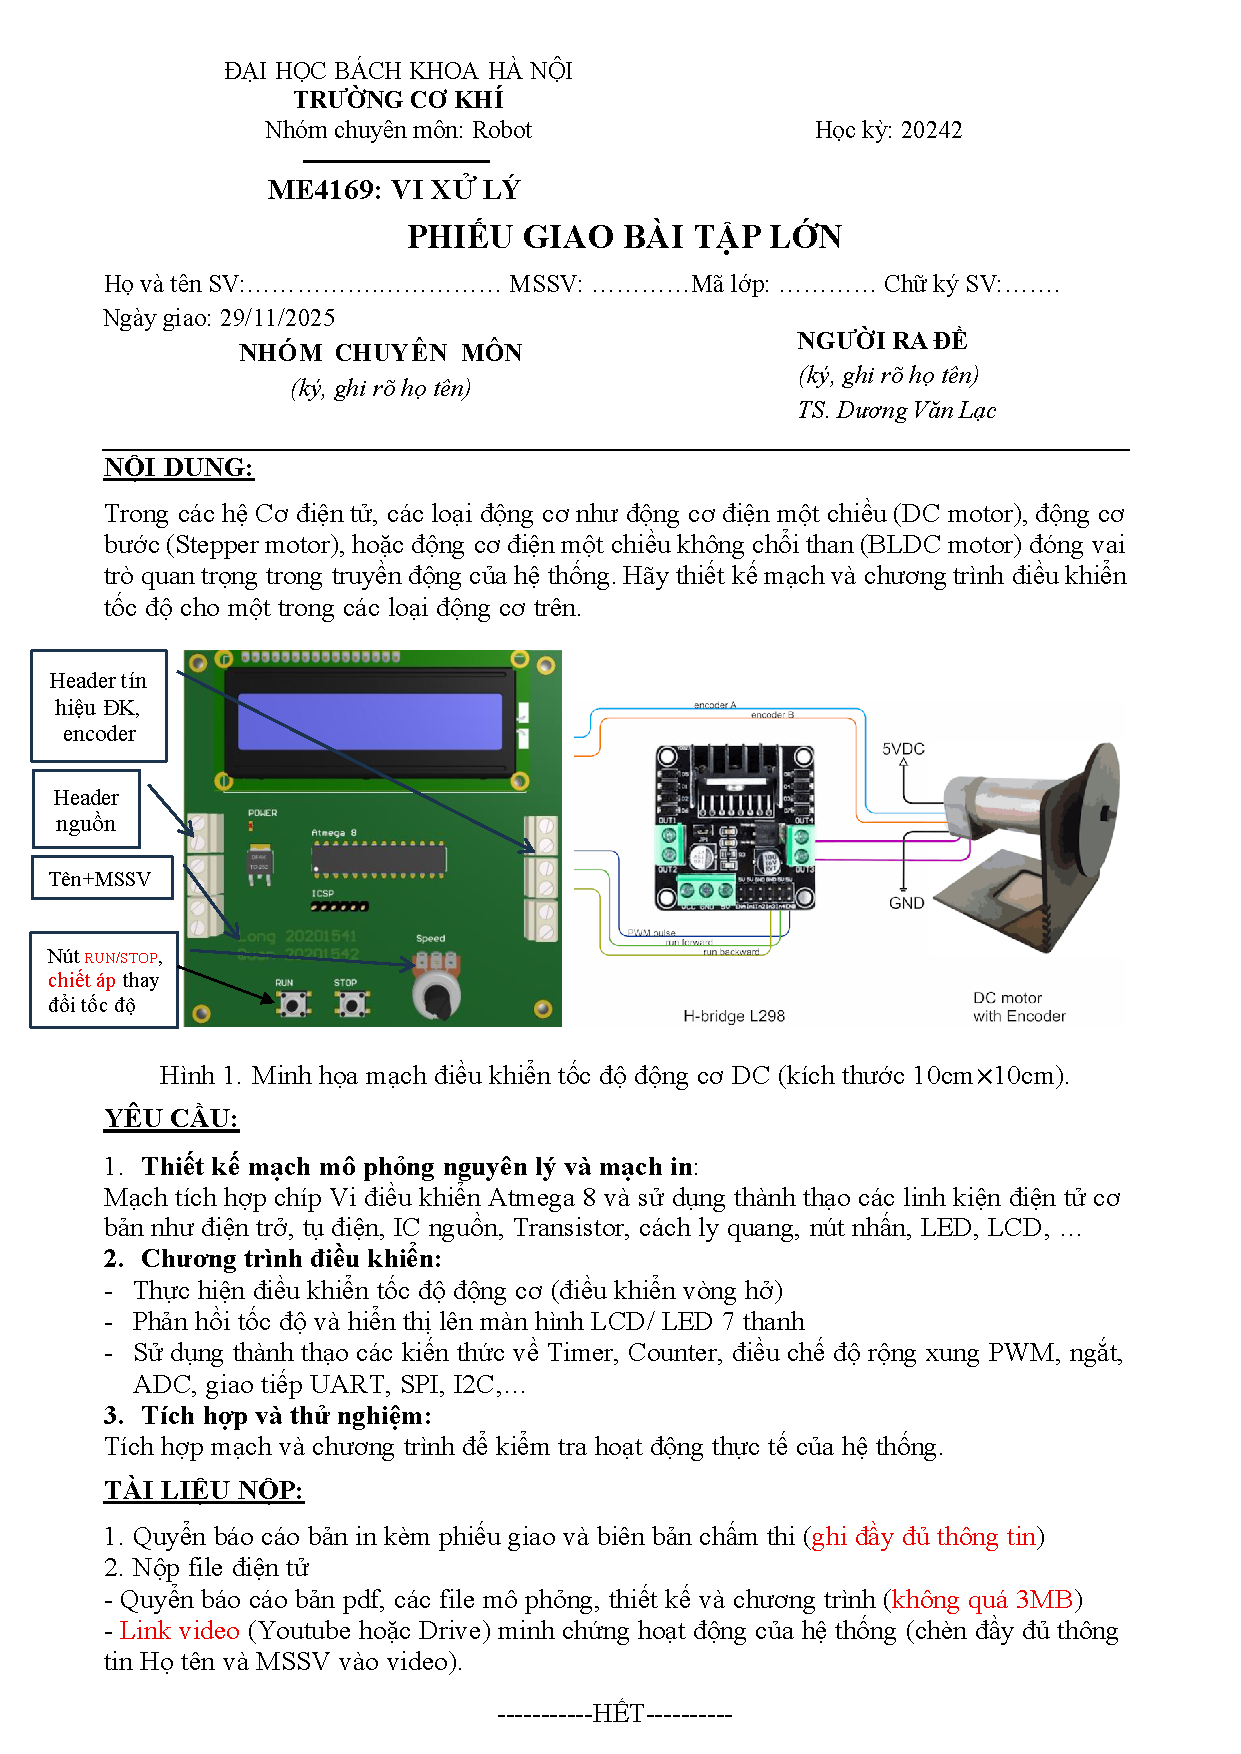
\includegraphics[page=1, width=1\linewidth]{figures/ME4169_DEBAI.pdf}
\end{figure}
\addcontentsline{toc}{chapter}{Đề bài học phần}
\clearpage

% ============================ NỘI DUNG CHÍNH ============================
\pagenumbering{arabic}
%!TEX root = ./main.tex
%!TEX program = xelatex
% =====================================================================
%  01 - GIỚI THIỆU
% =====================================================================
\chapter{Giới thiệu}
\label{ch:gioithieu}

\section{Điều khiển động cơ DC trong đời sống và công nghiệp}

\subsection{Động cơ DC và nhu cầu điều khiển tốc độ}
Động cơ DC có chổi than (brushed DC motor) có cấu tạo đơn giản, giá thành thấp, mô-men khởi động lớn và đặc biệt là dễ điều khiển: tốc độ gần như tỉ lệ thuận với điện áp phần ứng, còn chiều quay đổi khi đảo cực tính điện áp. Nhờ đó, chỉ cần một mạch cầu H (H-bridge) và tín hiệu điều khiển thích hợp (ví dụ: PWM) là có thể điều khiển cả tốc độ lẫn chiều quay.

Tuy nhiên, khi chạy vòng hở (open-loop) -- tức chỉ đặt một mức PWM cố định -- tốc độ thực tế sẽ thay đổi khi:
\begin{itemize}
  \item tải cơ khí thay đổi (băng tải thêm hàng, robot leo dốc\ldots);
  \item điện áp nguồn dao động (pin yếu dần, nguồn công nghiệp sụt áp);
  \item nhiệt độ cuộn dây tăng làm điện trở phần ứng thay đổi;
  \item sai khác giữa các động cơ cùng loại do dung sai chế tạo.
\end{itemize}
Để giữ tốc độ ổn định, hệ thống cần một cảm biến đo tốc độ (encoder, tachometer, cảm biến Hall) và một bộ điều khiển phản hồi -- phổ biến nhất là bộ điều khiển PID. Đây là cấu trúc điều khiển vòng kín (closed-loop control).

\subsection{Ứng dụng trong đời sống}
\begin{itemize}
  \item \textbf{Thiết bị gia dụng:} máy xay sinh tố nhiều cấp tốc độ, máy hút bụi, quạt điều tốc, máy pha cà phê, bàn chải đánh răng điện.
  \item \textbf{Ô tô và xe điện cá nhân:} bơm nhiên liệu, quạt làm mát, gạt mưa, chỉnh ghế, cửa kính điện, xe đạp/xe scooter điện.
  \item \textbf{Thiết bị văn phòng và tiêu dùng:} máy in, máy quét, ổ đĩa, đồ chơi điều khiển từ xa, drone cỡ nhỏ.
  \item \textbf{Y tế:} bơm tiêm điện, bơm truyền dịch, máy thở -- nơi lưu lượng phải chính xác nên bắt buộc điều khiển vòng kín.
  \item \textbf{Giáo dục và nghiên cứu:} robot dò line, robot tự cân bằng, mô hình thí nghiệm điều khiển tự động.
\end{itemize}

\subsection{Ứng dụng trong công nghiệp}
\begin{itemize}
  \item \textbf{Băng tải và hệ thống phân loại:} giữ tốc độ băng tải không đổi khi tải thay đổi để đồng bộ với camera, cảm biến và cơ cấu gắp.
  \item \textbf{Robot di động (AGV/AMR):} điều khiển tốc độ từng bánh xe để xe đi đúng quỹ đạo; tính toán quãng đường từ encoder (odometry).
  \item \textbf{Máy CNC, máy in 3D, cánh tay robot:} servo DC có encoder điều khiển vị trí và tốc độ chính xác.
  \item \textbf{Bơm, quạt, máy khuấy công nghiệp:} điều khiển lưu lượng/áp suất thông qua tốc độ động cơ, tiết kiệm năng lượng.
  \item \textbf{Dây chuyền cuốn -- nhả (winding):} điều khiển tốc độ và lực căng cho giấy, màng nhựa, dây cáp.
\end{itemize}
Trong công nghiệp, các chức năng trên thường được đảm nhiệm bởi bộ điều khiển động cơ (motor driver/controller) chuyên dụng, nhận lệnh từ PLC hoặc máy tính qua tín hiệu tương tự (0--10 V, chiết áp), xung PWM hoặc các bus truyền thông (UART/RS-485, CAN, Modbus). Một bộ điều khiển như vậy luôn có các khối: nguồn và bảo vệ, tầng công suất, đo phản hồi, bộ xử lý chạy thuật toán điều khiển, giao diện người dùng và giao tiếp. \proj{} được thiết kế đúng theo cấu trúc đó, ở quy mô thu nhỏ phù hợp với một đề tài học phần.

\section{Tổng quan về \proj}

\subsection{\proj{} là gì?}
\textbf{\proj} là một \textbf{bộ điều khiển tốc độ động cơ DC có chổi than, vòng kín, một kênh}, được xây dựng trên vi điều khiển AVR 8-bit \textbf{ATmega88PA} chạy ở \SI{16}{\mega\hertz}. Toàn bộ hệ thống nằm trên một bo mạch in 2 lớp kích thước 80\,$\times$\,60\,mm, sử dụng một nguồn duy nhất \SI{12}{\volt} DC.

Tên gọi ``UniDrive'' (\emph{Universal Drive}) thể hiện định hướng của nhóm: một bộ điều khiển \emph{đa dụng}, có thể dùng cho nhiều loại động cơ DC có encoder khác nhau chỉ bằng cách thay đổi các thông số trong một tệp cấu hình duy nhất (\texttt{config.h}). Hậu tố ``Lite'' cho biết đây là phiên bản rút gọn, đặt nền móng cho phiên bản đầy đủ \projpro{} (xem Chương~\ref{ch:ketluan}).

\subsection{\proj{} làm được gì?}
\begin{itemize}
  \item \textbf{Điều khiển tốc độ vòng kín} bằng bộ PID số dấu phẩy tĩnh (Q8) có bù thuận (feed-forward), giới hạn gia tốc (setpoint ramp), chống bão hòa tích phân (anti-windup) và lọc thành phần vi phân.
  \item \textbf{Điều khiển hai chiều quay}, dải đặt tốc độ $\pm\SI{2700}{rpm}$ (cấu hình được).
  \item \textbf{Đo tốc độ} bằng encoder cầu phương, giải mã $\times4$, có bộ lọc số chống nhiễu kiểu ``STM32 input filter''.
  \item \textbf{Hai chế độ đặt tốc độ:}
    \begin{itemize}
      \item \emph{POTENTIOMETER} -- xoay chiết áp: vị trí giữa là \SI{0}{rpm}, xoay về hai phía để đổi chiều quay;
      \item \emph{UART} -- gửi lệnh số nguyên từ máy tính/PLC/vi điều khiển khác ở \SI{115200}{baud}.
    \end{itemize}
  \item \textbf{Giao diện người dùng:} 2 nút nhấn RUN/STOP (nhấn ngắn/nhấn giữ), 2 LED trạng thái và màn hình TFT màu 1,8\,inch hiển thị chế độ, trạng thái, tốc độ đặt và tốc độ đo được.
  \item \textbf{Bảo vệ:} chống ngược cực nguồn bằng P-MOSFET, các bảo vệ quá dòng/quá nhiệt/thấp áp tích hợp trong IC công suất, chế độ ngủ (sleep) ngắt hoàn toàn tầng công suất khi dừng.
\end{itemize}

\section{Sơ đồ khối phần cứng}

Hình~\ref{fig:sodokhoi} trình bày sơ đồ khối phần cứng của \proj. Hệ thống gồm năm nhóm chức năng: \textcolor{hustred}{\textbf{nguồn}}, \textcolor{blk}{\textbf{xử lý trung tâm}}, \textbf{tầng công suất}, \textcolor{green!40!black}{\textbf{giao diện vào/ra}} và \textbf{giao tiếp/nạp chương trình}.

\begin{figure}[H]
\centering
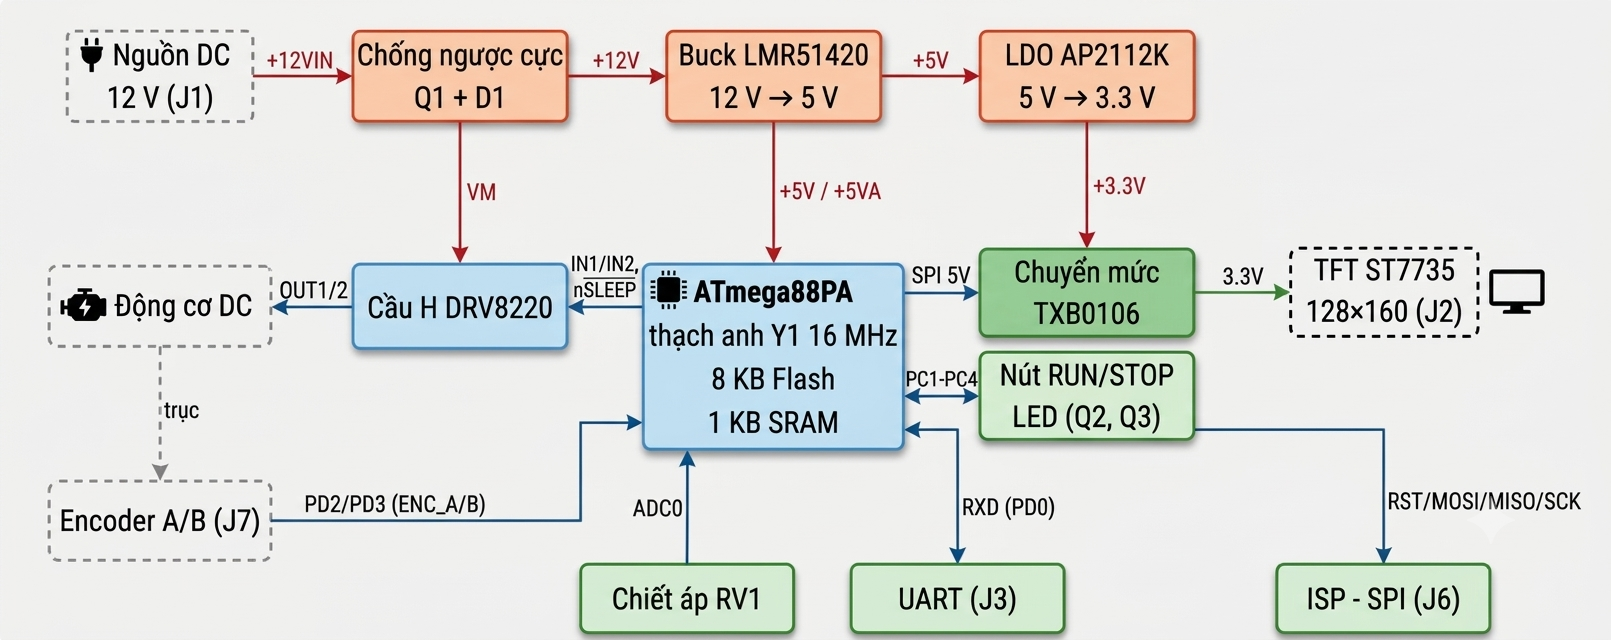
\includegraphics[width=\linewidth]{figures/SODOKHOIHARDWARE.png}
\caption{Sơ đồ khối phần cứng của \proj}
\label{fig:sodokhoi}
\end{figure}

\begin{figure}[H]
\centering
\begin{subfigure}{0.49\linewidth}\centering\hinh[\linewidth]{figures/3D_Front.png}{Ảnh 3D mặt trên}\caption{Mặt trên}\end{subfigure}
\hfill
\begin{subfigure}{0.49\linewidth}\centering\hinh[\linewidth]{figures/3D_Back.png}{Ảnh 3D mặt dưới}\caption{Mặt dưới}\end{subfigure}
\caption{Mô hình 3D bo mạch \proj{} (xuất từ KiCad)}
\label{fig:3d}
\end{figure}

\section{Danh sách linh kiện}

Bảng~\ref{tab:bom} liệt kê các linh kiện chính, được nhóm theo khối chức năng. Danh sách đầy đủ (bao gồm tụ, trở thụ động) được trích trực tiếp từ sơ đồ nguyên lý KiCad.

\begin{longtable}{@{}p{2.6cm}p{3.4cm}p{3.4cm}c p{3.4cm}@{}}
\caption{Danh sách linh kiện (BOM) của \proj}\label{tab:bom}\\
\toprule
\textbf{Ký hiệu} & \textbf{Giá trị / Mã} & \textbf{Vỏ (footprint)} & \textbf{SL} & \textbf{Chức năng}\\
\midrule\endfirsthead
\toprule
\textbf{Ký hiệu} & \textbf{Giá trị / Mã} & \textbf{Vỏ (footprint)} & \textbf{SL} & \textbf{Chức năng}\\
\midrule\endhead
\bottomrule\endfoot
\multicolumn{5}{@{}l}{\cellcolor{blkfill}\textit{Khối xử lý trung tâm}}\\
U2 & ATmega88PA-A & TQFP-32 & 1 & Vi điều khiển chính\\
Y1 & \SI{16}{\mega\hertz} & SMD 3225 & 1 & Thạch anh dao động\\
C7, C8 & \SI{22}{\pico\farad} & 0603 & 2 & Tụ tải thạch anh\\
L1 / R1 & \SI{10}{\micro\henry} / \SI{22}{\ohm} & 0603 & 2 & Lọc nguồn AVCC (+5VA)\\
C1--C3, C6 & \SI{100}{\nano\farad}, \SI{10}{\nano\farad} & 0603 & 4 & Tụ thoát VCC/AVCC/AREF\\
SW3, R6, C21 & Nút nhấn, \SI{10}{\kilo\ohm}, \SI{100}{\nano\farad} & B3F, 0603 & 3 & Mạch RESET\\
\multicolumn{5}{@{}l}{\cellcolor{pwrfill}\textit{Khối nguồn và bảo vệ}}\\
Q1 & CSD25404Q3 & VSON-8 3,3$\times$3,3 & 1 & P-MOSFET chống ngược cực\\
D1 & BZT52C10 & SOD-123 & 1 & Zener kẹp $V_{GS}$ của Q1\\
R2 & \SI{100}{\kilo\ohm} & 0603 & 1 & Điện trở cực cổng Q1\\
U1 & LMR51420XFDDCR & SOT-23-6 & 1 & Buck đồng bộ \SI{12}{\volt}$\to$\SI{5}{\volt}\\
L2 & \SI{10}{\micro\henry} & IHLP-1616 & 1 & Cuộn cảm buck\\
R5, R7 & \SI{100}{\kilo\ohm}, \SI{13.7}{\kilo\ohm} & 0603 & 2 & Cầu phân áp hồi tiếp (FB)\\
C9, C10, C11, C12 & \SI{100}{\nano\farad}, \SI{2.2}{\micro\farad}, 2$\times$\SI{22}{\micro\farad} & 0603/1206 & 4 & Bootstrap, tụ vào, tụ ra\\
U3 & AP2112K-3.3 & SOT-23-5 & 1 & LDO \SI{3.3}{\volt} / \SI{600}{\milli\ampere}\\
C13, C14 & \SI{22}{\micro\farad} & 1206 & 2 & Tụ vào/ra LDO\\
C4, C17 & \SI{220}{\micro\farad} & Hóa 6,3$\times$7,7 & 2 & Tụ bulk bus \SI{12}{\volt}\\
\multicolumn{5}{@{}l}{\cellcolor{blkfill}\textit{Khối công suất}}\\
U5 & DRV8220DSG & WSON-8 2$\times$2 & 1 & Cầu H \SI{18}{\volt}/\SI{1.76}{\ampere}\\
JP1, R10 & Jumper hàn, \SI{10}{\kilo\ohm} & -- & 2 & Chọn chế độ PWM / PH-EN\\
C18 & \SI{100}{\nano\farad} & 0603 & 1 & Tụ thoát VM\\
M1 & Domino 2 chân & MKDS 5,08 & 1 & Đầu ra động cơ\\
\multicolumn{5}{@{}l}{\cellcolor{iofill}\textit{Khối giao diện}}\\
U4 & TXB0106RGY & VQFN-16 & 1 & Chuyển mức \SI{5}{\volt}$\leftrightarrow$\SI{3.3}{\volt} cho TFT\\
R9, R12 & \SI{30.1}{\kilo\ohm}, \SI{60.4}{\kilo\ohm} & 0603 & 2 & Phân áp chân OE\\
C15, C16 & \SI{100}{\nano\farad} & 0603 & 2 & Tụ thoát VCCA/VCCB\\
RV1 & Chiết áp Alps RK097 & -- & 1 & Đặt tốc độ\\
SW1, SW2 & Nút nhấn Omron B3F & -- & 2 & Nút RUN, STOP\\
R3, R4, C19, C20 & \SI{10}{\kilo\ohm}, \SI{100}{\nano\farad} & 0603 & 4 & Kéo xuống + lọc RC nút nhấn\\
D2, D3 & LED & 1206 & 2 & LED STOP, RUN\\
Q2, Q3 & 2N7002 & SOT-23 & 2 & Khóa LED\\
R8, R11, R13--R16 & \SI{10}{\kilo\ohm}, \SI{22}{\ohm} & 0603 & 6 & Trở hạn dòng LED, trở cổng\\
\multicolumn{5}{@{}l}{\cellcolor{swfill}\textit{Đầu nối và cơ khí}}\\
J1 & Domino 2 chân & MKDS 5,08 & 1 & Đầu vào nguồn \SI{12}{\volt}\\
J2 & Header cái 1$\times$8 & 2,54 mm & 1 & Module TFT WeAct ST7735\\
J3 & JST-XH 4 chân & 2,50 mm & 1 & UART\\
J6 & JST-XH 5 chân & 2,50 mm & 1 & Nạp ISP\\
J7 & JST-XH 4 chân & 2,50 mm & 1 & Encoder\\
J4, J5 & Header 1$\times$3 & 2,54 mm & 2 & Đầu chờ +5V / GND\\
TP1--TP7 & Test point & $\varnothing$\SI{1}{\milli\metre} & 7 & Điểm đo\\
H1--H4 & Lỗ M3 & $\varnothing$\SI{3.2}{\milli\metre} & 4 & Lỗ bắt vít\\
\end{longtable}

\section{Thông số kỹ thuật}
\label{sec:thongso}

Phần này trình bày thông số của \proj{}. Các giới hạn được suy ra từ datasheet của linh kiện yếu nhất trong mỗi đường tín hiệu; các thông số chức năng được tính từ cấu hình firmware mặc định trong \texttt{config.h}.

\begin{tcolorbox}[colback=white,colframe=hustred,title={\bfseries UNIDRIVE LITE -- Single-Channel Closed-Loop Brushed DC Motor Controller},fonttitle=\large]
\begin{minipage}[t]{0.48\linewidth}
\textbf{Đặc điểm nổi bật}
\begin{itemize}[leftmargin=*,itemsep=0pt]
  \item Nguồn vào đơn \SIrange{7}{16}{\volt}, danh định \SI{12}{\volt}
  \item Chống ngược cực nguồn
  \item Dòng động cơ đỉnh \SI{1.76}{\ampere}
  \item PID dấu phẩy tĩnh, chu kỳ \SI{50}{\milli\second}
  \item Encoder $\times4$ có lọc nhiễu số
\end{itemize}
\end{minipage}\hfill
\begin{minipage}[t]{0.48\linewidth}
\textbf{\phantom{x}}
\begin{itemize}[leftmargin=*,itemsep=0pt]
  \item Đặt tốc độ: chiết áp / UART
  \item Màn hình TFT màu 128$\times$160
  \item Cấu hình tập trung trong \texttt{config.h}
  \item Bo mạch 2 lớp 80\,$\times$\,60\,mm
  \item Nạp chương trình qua ISP (SPI)
\end{itemize}
\end{minipage}
\end{tcolorbox}

\subsection{Giới hạn tuyệt đối (Absolute Maximum Ratings)}
\begin{table}[H]
\centering\small
\caption{Giới hạn tuyệt đối -- vượt quá có thể làm hỏng thiết bị}
\label{tab:absmax}
\begin{tabularx}{\linewidth}{@{}Xccc>{\raggedright\arraybackslash}p{4.2cm}@{}}
\toprule
\textbf{Thông số} & \textbf{Min} & \textbf{Max} & \textbf{Đơn vị} & \textbf{Giới hạn bởi}\\
\midrule
Điện áp vào $V_{IN}$ (J1) & $-20$ & 20 & \si{\volt} & $V_{DS}$ Q1, $V_{M}$ DRV8220\\
Dòng ra động cơ (đỉnh) & -- & 1,76 & \si{\ampere} & Giới hạn dòng DRV8220\\
Tải trên đường \SI{5}{\volt} (J4) & -- & 2 & \si{\ampere} & LMR51420 (gồm tải nội)\\
Tải trên đường \SI{3.3}{\volt} & -- & 0,6 & \si{\ampere} & AP2112K\\
Điện áp chân tín hiệu J3, J7 & $-0,5$ & 5,5 & \si{\volt} & ATmega88PA ($V_{CC}+0,5$)\\
Điện áp chân MODE (DRV8220) & -- & 5,75 & \si{\volt} & DRV8220\\
Nhiệt độ làm việc & $-20$ & 85 & \si{\celsius} & Linh kiện thương mại\\
\bottomrule
\end{tabularx}
\end{table}

\subsection{Điều kiện làm việc khuyến nghị}
\begin{table}[H]
\centering\small
\caption{Điều kiện làm việc khuyến nghị}
\label{tab:recommended}
\begin{tabularx}{\linewidth}{@{}Xcccc@{}}
\toprule
\textbf{Thông số} & \textbf{Min} & \textbf{Typ} & \textbf{Max} & \textbf{Đơn vị}\\
\midrule
Điện áp vào $V_{IN}$ (in trên bo: MAX 16\,VDC) & 7 & 12 & 16 & \si{\volt}\\
Dòng động cơ liên tục & -- & -- & 1,0 & \si{\ampere}\\
Điện áp định mức động cơ & -- & $V_{IN}$ & -- & \si{\volt}\\
Độ phân giải encoder  & 1 & 20 & 500 & PPR\\
Tần số mỗi kênh encoder (khi bật lọc) & 0 & -- & 5 & \si{\kilo\hertz}\\
\bottomrule
\end{tabularx}
\end{table}

\subsection{Đặc tính điện}
\begin{table}[H]
\centering\small
\caption{Đặc tính điện ($V_{IN}=\SI{12}{\volt}$, $T_A=\SI{25}{\celsius}$, cấu hình mặc định)}
\label{tab:electrical}
\begin{tabularx}{\linewidth}{@{}>{\raggedright\arraybackslash}Xp{3.6cm}cccc@{}}
\toprule
\textbf{Thông số} & \textbf{Điều kiện} & \textbf{Min} & \textbf{Typ} & \textbf{Max} & \textbf{Đơn vị}\\
\midrule
\multicolumn{6}{@{}l}{\textit{Nguồn}}\\
Điện áp đường +5V & $I_{OUT}\le\SI{1}{\ampere}$ & 4,92 & 4,98 & 5,05 & \si{\volt}\\
Điện áp đường +3.3V & -- & 3,23 & 3,30 & 3,37 & \si{\volt}\\
Tần số chuyển mạch buck & FPWM & -- & 500 & -- & \si{\kilo\hertz}\\
Sụt áp chống ngược cực & $I=\SI{1}{\ampere}$ & -- & 5,5 & -- & \si{\milli\volt}\\
Dòng tiêu thụ khi STOP & Động cơ ngủ & -- & \bosung{đo} & -- & \si{\milli\ampere}\\
\multicolumn{6}{@{}l}{\textit{Tầng công suất}}\\
Tần số PWM & Timer2, chia 32 & -- & 1953 & -- & \si{\hertz}\\
Độ phân giải PWM & -- & -- & 8 & -- & bit\\
Chế độ suy giảm dòng & Mặc định & \multicolumn{3}{c}{Slow decay (hãm)} & --\\
\multicolumn{6}{@{}l}{\textit{Đo lường và điều khiển}}\\
Dải đặt tốc độ & \texttt{APP\_MAX\_RPM} & $-2700$ & -- & 2700 & \si{rpm}\\
Độ phân giải đo tốc độ & 20 PPR, cửa sổ \SI{50}{\milli\second} & -- & 15 & -- & \si{rpm}\\
Chu kỳ vòng điều khiển & \texttt{MOTION\_PERIOD\_MS} & -- & 50 & -- & \si{\milli\second}\\
Giới hạn gia tốc đặt & \texttt{MOTION\_ACCEL} & -- & 6000 & -- & \si{rpm\per\second}\\
Độ rộng xung nhiễu bị loại & $N=4$, \SI{80}{\kilo\hertz} & -- & 50 & -- & \si{\micro\second}\\
\multicolumn{6}{@{}l}{\textit{Giao diện}}\\
Tốc độ UART & 8N1, chỉ nhận & -- & 115200 & -- & baud\\
Sai số tốc độ baud & U2X, UBRR = 16 & -- & +2,1 & -- & \%\\
Độ phân giải ADC chiết áp & Tham chiếu AVCC & -- & 10 & -- & bit\\
Thời gian chống dội nút & -- & -- & 20 & -- & \si{\milli\second}\\
Thời gian nhấn giữ & -- & -- & 2000 & -- & \si{\milli\second}\\
Xung nhịp SPI tới TFT & $f_{osc}/2$ & -- & 8 & -- & \si{\mega\hertz}\\
\bottomrule
\end{tabularx}
\end{table}

\subsection{Sơ đồ chân đầu nối}
\begin{table}[H]
\centering\small
\caption{Sơ đồ chân các đầu nối trên bo mạch}
\label{tab:connectors}
\begin{tabularx}{\linewidth}{@{}l>{\raggedright\arraybackslash}p{2.8cm}c>{\raggedright\arraybackslash}X@{}}
\toprule
\textbf{Đầu nối} & \textbf{Chức năng} & \textbf{Chân} & \textbf{Tín hiệu}\\
\midrule
J1 & Nguồn vào & 1 / 2 & +12VIN / GND\\
M1 & Động cơ & 1 / 2 & OUT1 (+) / OUT2 ($-$)\\
J2 & TFT ST7735 & 1--8 & GND, +5V, SCK, SDA, RST, DC, CS, BL (mức \SI{3.3}{\volt})\\
J3 & UART & 1--4 & +5V, RX (PD0), GND, TX (PD1)\\
J6 & ISP & 1--5 & RESET, MOSI, MISO, SCK, GND \textit{(không cấp nguồn)}\\
J7 & Encoder & 1--4 & +5V, ENC\_A (PD2), ENC\_B (PD3), GND\\
J4 / J5 & Đầu chờ & 1--3 & +5V / GND\\
\bottomrule
\end{tabularx}
\end{table}

\subsection{Phân bố chân vi điều khiển}
\begin{table}[H]
\centering\small
\caption{Phân bố chân ATmega88PA}
\label{tab:pinmap}
\begin{tabular}{@{}lll|lll@{}}
\toprule
\textbf{Chân} & \textbf{Tín hiệu} & \textbf{Ngoại vi} & \textbf{Chân} & \textbf{Tín hiệu} & \textbf{Ngoại vi}\\
\midrule
PB0 & TFT\_RST & GPIO & PD0 & UART RX & USART0\\
PB1 & TFT\_BL & GPIO & PD2 & ENC\_A & Timer1 lấy mẫu\\
PB2 & TFT\_CS & GPIO & PD3 & ENC\_B & Timer1 lấy mẫu\\
PB3 & TFT\_MOSI & SPI & PD4 & nSLEEP & GPIO\\
PB5 & TFT\_SCK & SPI & PD5 & IN1/PH & PWM mềm Timer2\\
PB6/PB7 & XTAL1/2 & Thạch anh & PD6 & IN2/EN & PWM mềm Timer2\\
PC0 & Chiết áp & ADC0 & PD7 & TFT\_DC & GPIO\\
PC1 / PC3 & Nút RUN / STOP & GPIO & PC6 & RESET & ISP\\
PC2 / PC4 & LED RUN / STOP & GPIO & ADC6 & OE\_CONTROL & (xem mục~\ref{sec:hanche})\\
\bottomrule
\end{tabular}
\end{table}

%!TEX root = ./main.tex
%!TEX program = xelatex
% =====================================================================
%  02 - QUÁ TRÌNH THIẾT KẾ PHẦN CỨNG
% =====================================================================
\chapter{Quá trình thiết kế phần cứng}
\label{ch:thietke}

\section{Quy trình thiết kế tổng thể}

Phần cứng của \proj{} được phát triển theo quy trình ``chữ V'' rút gọn: bắt đầu từ yêu cầu chức năng, đi xuống thiết kế chi tiết từng khối, sau đó đi lên qua chế tạo, lắp ráp và kiểm thử từng khối trước khi tích hợp toàn hệ thống (Hình~\ref{fig:quytrinh}). Toàn bộ thiết kế điện tử được thực hiện trên phần mềm mã nguồn mở \textbf{KiCad}.

\begin{figure}[H]
\centering
\resizebox{\linewidth}{!}{%
\begin{tikzpicture}[
  st/.style={draw=blk,thick,rounded corners=3pt,fill=blkfill,minimum width=34mm,minimum height=9mm,align=center,font=\small},
  ar/.style={-{Stealth[length=2.5mm]},thick}]
  \node[st] (a) at (0,0) {1. Xác định yêu cầu};
  \node[st] (b) at (1.4,-1.3) {2. Kiến trúc \& sơ đồ khối};
  \node[st] (c) at (2.8,-2.6) {3. Chọn linh kiện};
  \node[st] (d) at (4.2,-3.9) {4. Sơ đồ nguyên lý};
  \node[st,fill=swfill] (e) at (7,-5.2) {5. Bố trí \& đi dây PCB};
  \node[st] (f) at (9.8,-3.9) {6. DRC, xuất Gerber};
  \node[st] (g) at (11.2,-2.6) {7. Gia công \& hàn};
  \node[st] (h) at (12.6,-1.3) {8. Kiểm tra từng khối};
  \node[st] (i) at (14,0) {9. Tích hợp firmware};
  \foreach \x/\y in {a/b,b/c,c/d,d/e,e/f,f/g,g/h,h/i} \draw[ar] (\x) -- (\y);
  \draw[ar,dashed,gray] (h.north west) to[bend right=20] node[above,font=\scriptsize]{sửa lỗi} (d.north east);
\end{tikzpicture}}
\caption{Quy trình thiết kế phần cứng \proj}
\label{fig:quytrinh}
\end{figure}

\subsection{Yêu cầu thiết kế}
Từ mục tiêu đề tài, nhóm đặt ra các yêu cầu sau làm cơ sở cho mọi quyết định thiết kế:
\begin{enumerate}[label=\textbf{R\arabic*.}]
  \item Dùng \textbf{một nguồn duy nhất} \SI{12}{\volt} cho cả động cơ và mạch điều khiển.
  \item Điều khiển động cơ DC \SI{12}{\volt} \textbf{hai chiều}, dòng tới khoảng \SI{1}{\ampere}.
  \item Đọc encoder, \textbf{điều khiển vòng kín} bằng PID.
  \item Đặt tốc độ bằng \textbf{chiết áp} hoặc \textbf{UART}.
  \item Có \textbf{giao diện người dùng}: nút nhấn, LED, màn hình.
  \item \textbf{Bảo vệ} khi cắm ngược nguồn; ngắt tầng công suất khi dừng.
  \item Nạp được chương trình \textbf{không cần bootloader} (ISP), có điểm đo (test point) cho việc gỡ lỗi.
  \item Bo mạch \textbf{nhỏ gọn}, 2 lớp, linh kiện dán (SMD) phổ biến, dễ đặt gia công.
\end{enumerate}

\section{Lựa chọn linh kiện}

\subsection{Vi điều khiển: ATmega88PA}
\begin{table}[H]
\centering\small
\caption{So sánh các phương án vi điều khiển}
\label{tab:sosanh_mcu}
\begin{tabularx}{\linewidth}{@{}l>{\centering\arraybackslash}X>{\centering\arraybackslash}X>{\centering\arraybackslash}X@{}}
\toprule
\textbf{Tiêu chí} & \textbf{ATmega88PA} & \textbf{ATmega328P} & \textbf{STM32F103}\\
\midrule
Kiến trúc & AVR 8-bit & AVR 8-bit & ARM Cortex-M3 32-bit\\
Flash / SRAM & 8\,KB / 1\,KB & 32\,KB / 2\,KB & 64\,KB / 20\,KB\\
Điện áp & \SIrange{1.8}{5.5}{\volt} & \SIrange{1.8}{5.5}{\volt} & \SIrange{2}{3.6}{\volt}\\
Bộ giải mã encoder phần cứng & Không & Không & Có\\
Phù hợp nội dung học phần & Rất cao & Rất cao & Trung bình\\
Giá thành & Thấp & Trung bình & Trung bình\\
\bottomrule
\end{tabularx}
\end{table}

\begin{figure}[H]
\centering
\begin{subfigure}{0.49\linewidth}\centering\hinh[\linewidth]{figures/ATmega88PA_Front.jpg}{Ảnh MCU ATmega88PA mặt trên}\caption{Mặt trên}\end{subfigure}
\hfill
\begin{subfigure}{0.49\linewidth}\centering\hinh[\linewidth]{figures/ATmega88PA_Back.jpg}{Ảnh MCU ATmega88PA mặt dưới}\caption{Mặt dưới}\end{subfigure}
\caption{MCU ATmega88PA}
\label{fig:ATmega88PA}
\end{figure}

Nhóm chọn \textbf{ATmega88PA} vì: (i) cùng họ AVR với nội dung giảng dạy, tương thích chân với ATmega328P nên có thể nâng cấp bộ nhớ mà không sửa PCB; (ii) hoạt động ở \SI{5}{\volt}, tương thích trực tiếp với encoder, nút nhấn và đầu vào logic của DRV8220; (iii) chi phí thấp. Bộ nhớ 8\,KB Flash là một \emph{thử thách có chủ đích}: buộc nhóm phải viết firmware tối giản, thao tác trực tiếp thanh ghi thay vì dùng thư viện Arduino, vốn rất tốn dung lượng flash.

\subsection{IC Cầu H: DRV8220}
\begin{table}[H]
\centering\small
\caption{So sánh các phương án cầu H}
\label{tab:sosanh_drv}
\begin{tabularx}{\linewidth}{@{}l>{\centering\arraybackslash}X>{\centering\arraybackslash}X>{\centering\arraybackslash}X@{}}
\toprule
\textbf{Tiêu chí} & \textbf{L298N} & \textbf{TB6612FNG} & \textbf{DRV8220}\\
\midrule
Công nghệ & BJT & MOSFET & MOSFET\\
Điện áp động cơ & \SIrange{5}{46}{\volt} & \SIrange{2.5}{13.5}{\volt} & \SIrange{4.5}{18}{\volt}\\
Sụt áp / $R_{DS(on)}$ & $\sim$\SI{2}{\volt} & $\sim$\SI{0.5}{\ohm} & $\sim$\SI{1}{\ohm} (HS+LS)\\
Bảo vệ tích hợp & Không & Nhiệt & OCP, TSD, UVLO\\
Kích thước vỏ & Multiwatt-15 & SSOP-24 & WSON-8 2\,$\times$\,2\,mm\\
Chế độ ngủ & Không & Có & Có (dòng nA)\\
\bottomrule
\end{tabularx}
\end{table}

\begin{figure}[H]
\centering
\begin{subfigure}{0.49\linewidth}\centering\hinh[\linewidth]{figures/DRV8220DSG_Front.jpg}{Ảnh DRV8220 mặt trên}\caption{Mặt trên}\end{subfigure}
\hfill
\begin{subfigure}{0.49\linewidth}\centering\hinh[\linewidth]{figures/DRV8220DSG_Back.jpg}{Ảnh DRV8220 mặt dưới}\caption{Mặt dưới}\end{subfigure}
\caption{IC cầu H DRV8220}
\label{fig:drv8220}
\end{figure}

\textbf{DRV8220} được chọn vì phù hợp nguồn \SI{12}{\volt} (TB6612 chỉ tới \SI{13.5}{\volt}, sát giới hạn), có đầy đủ bảo vệ quá dòng, quá nhiệt, thấp áp, kích thước rất nhỏ (WSON-8 2x2mm), và có chân \texttt{nSLEEP} để ngắt hẳn tầng công suất -- đáp ứng yêu cầu R6. Ngoài ra, DRV8220 hỗ trợ hai chế độ giao tiếp IN1/IN2 (PWM) và PH/EN, được chọn bằng chân MODE; nhóm bố trí jumper hàn \textbf{JP1} cùng điện trở kéo xuống R10 để có thể chuyển chế độ mà không cần sửa mạch.

\subsection{Nguồn: buck LMR51420 + LDO AP2112K}
Mạch điều khiển cần đường \SI{5}{\volt} (MCU, encoder, logic) và \SI{3.3}{\volt} (màn hình TFT). Với dòng tải ước tính \SI{150}{\milli\ampere} trên đường \SI{5}{\volt}, nếu dùng ổn áp tuyến tính 7805 thì công suất tiêu tán:
\begin{equation}
  P_{7805}=(V_{IN}-V_{OUT})\cdot I=(12-5)\times0{,}15=\SI{1.05}{\watt},
\end{equation}
đòi hỏi tản nhiệt và lãng phí khoảng 58\,\% năng lượng. Nhóm chọn IC \textbf{buck LMR51420} (hiệu suất trên 85\,\%, package SOT-23-6, dòng ra tới \SI{2}{\ampere}, phiên bản \texttt{XF} chạy \SI{500}{\kilo\hertz} ở chế độ FPWM để tần số chuyển mạch cố định, dễ lọc nhiễu). Đường \SI{3.3}{\volt} chỉ cấp cho màn hình nên dùng LDO \textbf{AP2112K-3.3} (\SI{600}{\milli\ampere}, sụt áp thấp) nối sau đường \SI{5}{\volt} -- tổn hao chỉ $(5-3{,}3)\times I_{TFT}$, không đáng kể.

\begin{figure}[H]
\centering
\begin{subfigure}{0.49\linewidth}\centering\hinh[\linewidth]{figures/LMR51420.jpg}{Ảnh IC LMR51420}\caption{Ảnh IC LMR51420}\end{subfigure}
\hfill
\begin{subfigure}{0.49\linewidth}\centering\hinh[\linewidth]{figures/AP2112K.jpg}{Ảnh IC AP2112K}\caption{Ảnh IC AP2112K}\end{subfigure}
\caption{IC buck LMR51420 và LDO AP2112K}
\label{fig:lmr51420_ap2112k}
\end{figure}

\subsection{Chống ngược cực: P-MOSFET CSD25404Q3}
\begin{table}[H]
\centering\small
\caption{So sánh các phương án chống ngược cực tại $I=\SI{1}{\ampere}$}
\label{tab:sosanh_rpp}
\begin{tabular}{@{}lccc@{}}
\toprule
\textbf{Phương án} & \textbf{Sụt áp} & \textbf{Tổn hao} & \textbf{Ghi chú}\\
\midrule
Diode chỉnh lưu nối tiếp (1N5819) & $\sim$\SI{0.45}{\volt} & $\sim$\SI{0.45}{\watt} & Đơn giản, tổn hao lớn\\
Diode song song + cầu chì & 0 & 0 & Phải thay cầu chì sau sự cố\\
\textbf{P-MOSFET (CSD25404Q3)} & \textbf{\SI{5.5}{\milli\volt}} & \textbf{\SI{5.5}{\milli\watt}} & Tự phục hồi, gần như không tổn hao\\
\bottomrule
\end{tabular}
\end{table}

\begin{figure}[H]
\centering
\begin{subfigure}{0.45\linewidth}\centering\hinh[\linewidth]{figures/CSD25404Q3_Front.jpg}{Ảnh MOSFET CSD25404Q3}\caption{Mặt trên}\end{subfigure}
\hfill
\begin{subfigure}{0.45\linewidth}\centering\hinh[\linewidth]{figures/CSD25404Q3_Back.jpg}{Ảnh MOSFET CSD25404Q3}\caption{Mặt dưới}\end{subfigure}
\caption{P MOSFET CSD25404Q3}
\label{fig:CSD25404Q3}
\end{figure}

Nguyên lý: khi cắm đúng cực, dòng ban đầu chạy qua diode thân của Q1 làm cực nguồn S lên khoảng \SI{11.3}{\volt}, trong khi cực cổng G được R2 (\SI{100}{\kilo\ohm}) kéo về GND, nên $V_{GS}<0$ và MOSFET dẫn hoàn toàn. Zener \textbf{D1} (\SI{10}{\volt}) kẹp $|V_{GS}|\le\SI{10}{\volt}$, bảo vệ cực cổng (giới hạn $\pm\SI{12}{\volt}$) khi nguồn vào cao. Khi cắm ngược, $V_{GS}\ge0$, diode thân phân cực ngược và MOSFET khóa, mạch phía sau được cách ly.

\subsection{IC chuyển mức logic: TXB0106}

\begin{figure}[H]
\centering
\begin{subfigure}{0.45\linewidth}\centering\hinh[\linewidth]{figures/TXB0106_Front.jpg}{Ảnh IC TXB0106}\caption{Mặt trên}\end{subfigure}
\hfill
\begin{subfigure}{0.45\linewidth}\centering\hinh[\linewidth]{figures/TXB0106_Back.jpg}{Ảnh IC TXB0106}\caption{Mặt dưới}\end{subfigure}
\caption{IC chuyển mức logic TXB0106}
\label{fig:TXB0106}
\end{figure}

Module TFT WeAct ST7735 làm việc ở mức logic \SI{3.3}{\volt}, trong khi ATmega88PA xuất mức \SI{5}{\volt}. Nhóm dùng IC chuyển mức hai chiều tự nhận hướng \textbf{TXB0106} (6 kênh: SCK, MOSI, CS, DC, RST, BL) thay cho cầu phân áp điện trở, nhằm đảm bảo sườn xung SPI \SI{8}{\mega\hertz} sắc nét. Chân OE (tham chiếu theo $V_{CCA}=\SI{3.3}{\volt}$) được cấp qua cầu phân áp R9/R12:
\begin{equation}
  V_{OE}=V_{in}\cdot\frac{R_{12}}{R_9+R_{12}}=5\times\frac{60{,}4}{30{,}1+60{,}4}\approx\SI{3.34}{\volt}.
\end{equation}

\section{Thiết kế sơ đồ nguyên lý}

Sơ đồ nguyên lý được vẽ trên một trang A4, chia thành các vùng khối có tiêu đề theo đúng sơ đồ khối ở Hình~\ref{fig:sodokhoi}: \emph{Reverse Polarity Protection}, \emph{Power}, \emph{MCU}, \emph{IO}, \emph{Motor Driver}, \emph{LEDs}, \emph{Level Shifter}, \emph{Debug/UART/Encoder}. Sơ đồ đầy đủ được trình bày tại Phụ lục~\ref{app:schematic}. Một số tính toán chính:

\begin{figure}[H]
\centering
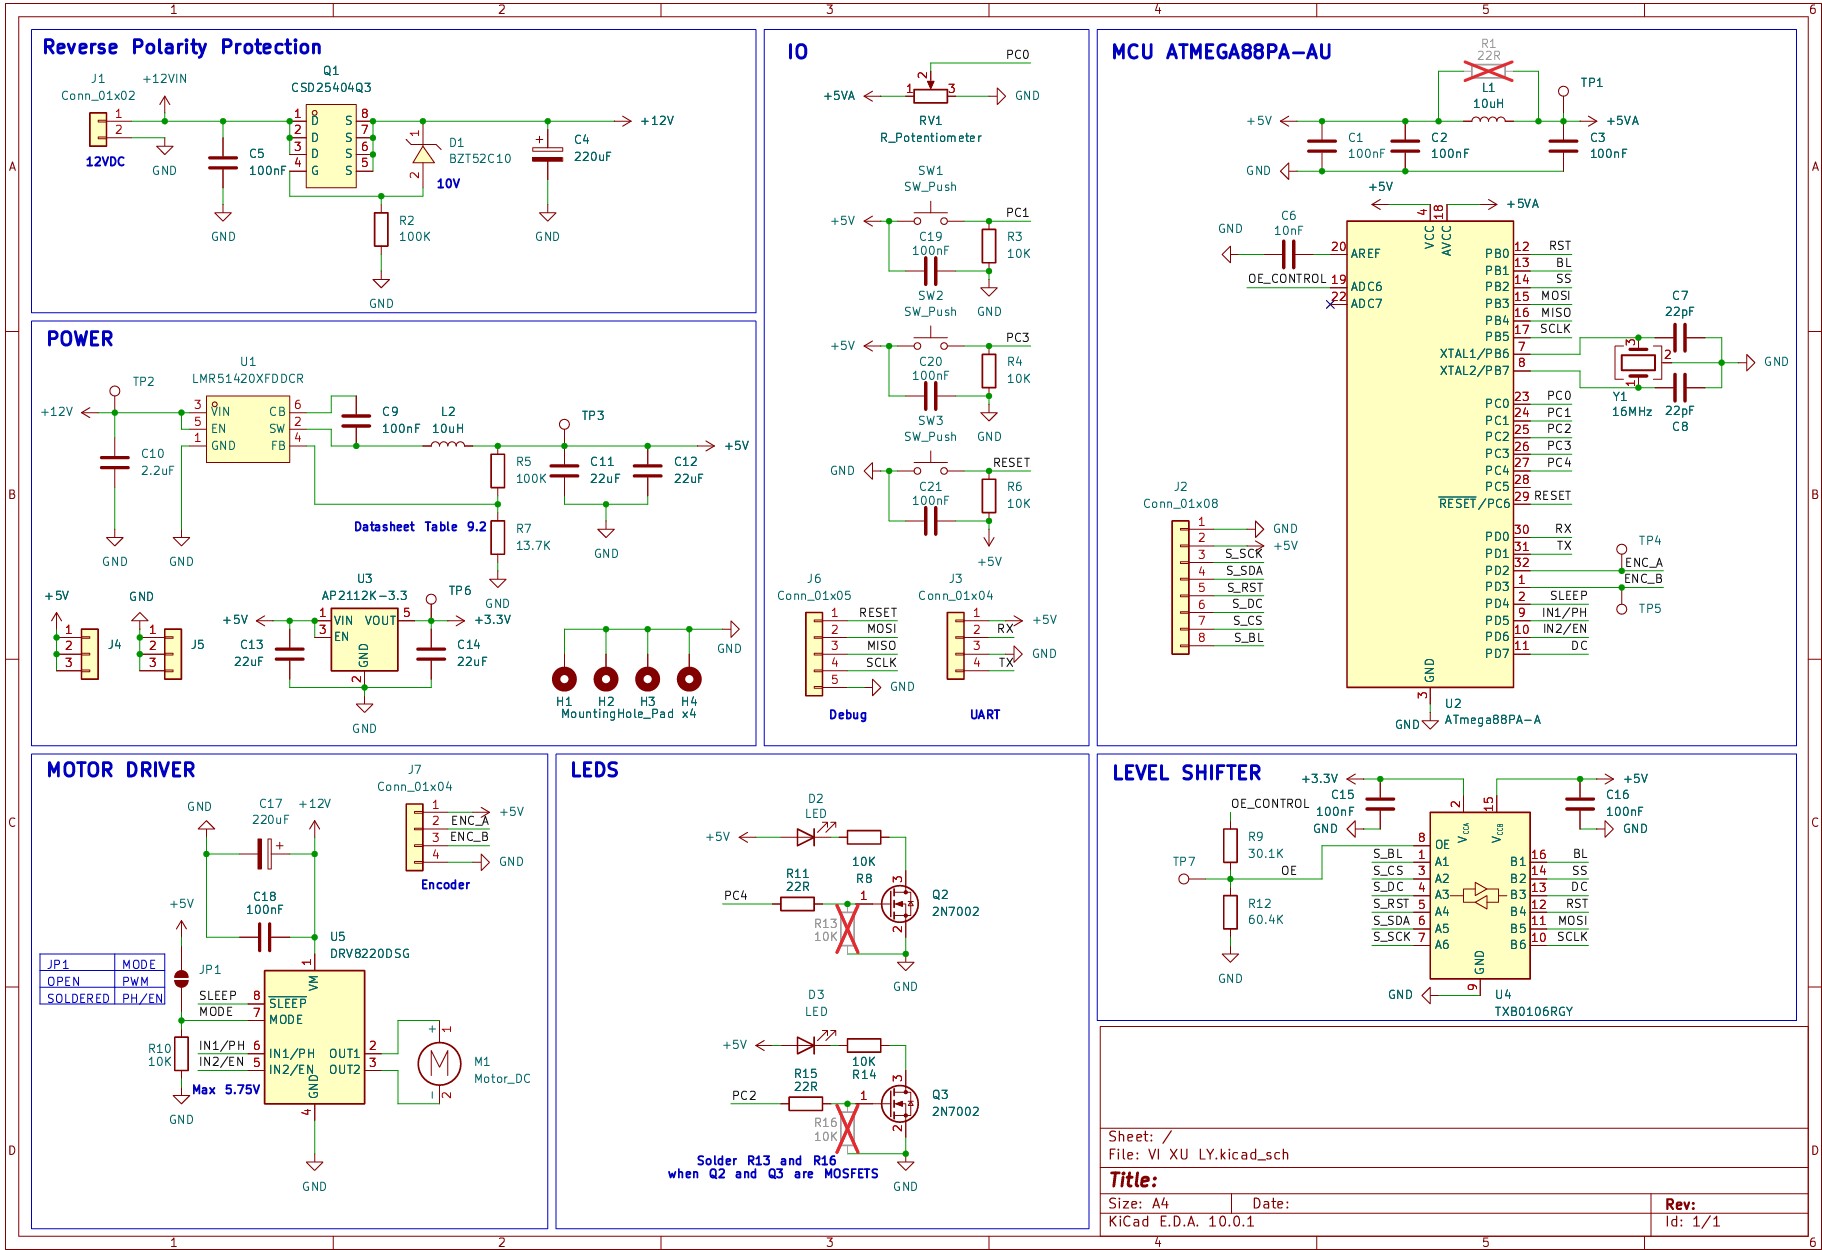
\includegraphics[width=\linewidth]{sch/SCH_PIC.png}
\caption{Sơ đồ nguyên lý \proj}
\label{fig:schematic}
\end{figure}

\paragraph{Mạch chống ngược cực.} P-MOSFET Q1 (CSD25404Q3) được đặt nối tiếp trên đường +12V từ đầu nối J1. Cực cổng được kéo xuống GND qua R2 (\SI{100}{\kilo\ohm}) nên khi cấp nguồn đúng cực, $V_{GS}\approx-\SI{12}{\volt}$ và MOSFET dẫn hoàn toàn; khi cắm ngược cực, $V_{GS}\ge0$ và MOSFET khóa, bảo vệ toàn bộ mạch phía sau. Zener D1 (BZT52C10) kẹp $|V_{GS}|$ ở \SI{10}{\volt}, dưới giới hạn tối đa của Q1. Tụ C5 (\SI{100}{\nano\farad}) và tụ hóa C4 (\SI{220}{\micro\farad}) lọc và dự trữ năng lượng cho bus +12V.

\begin{figure}[H]
\centering
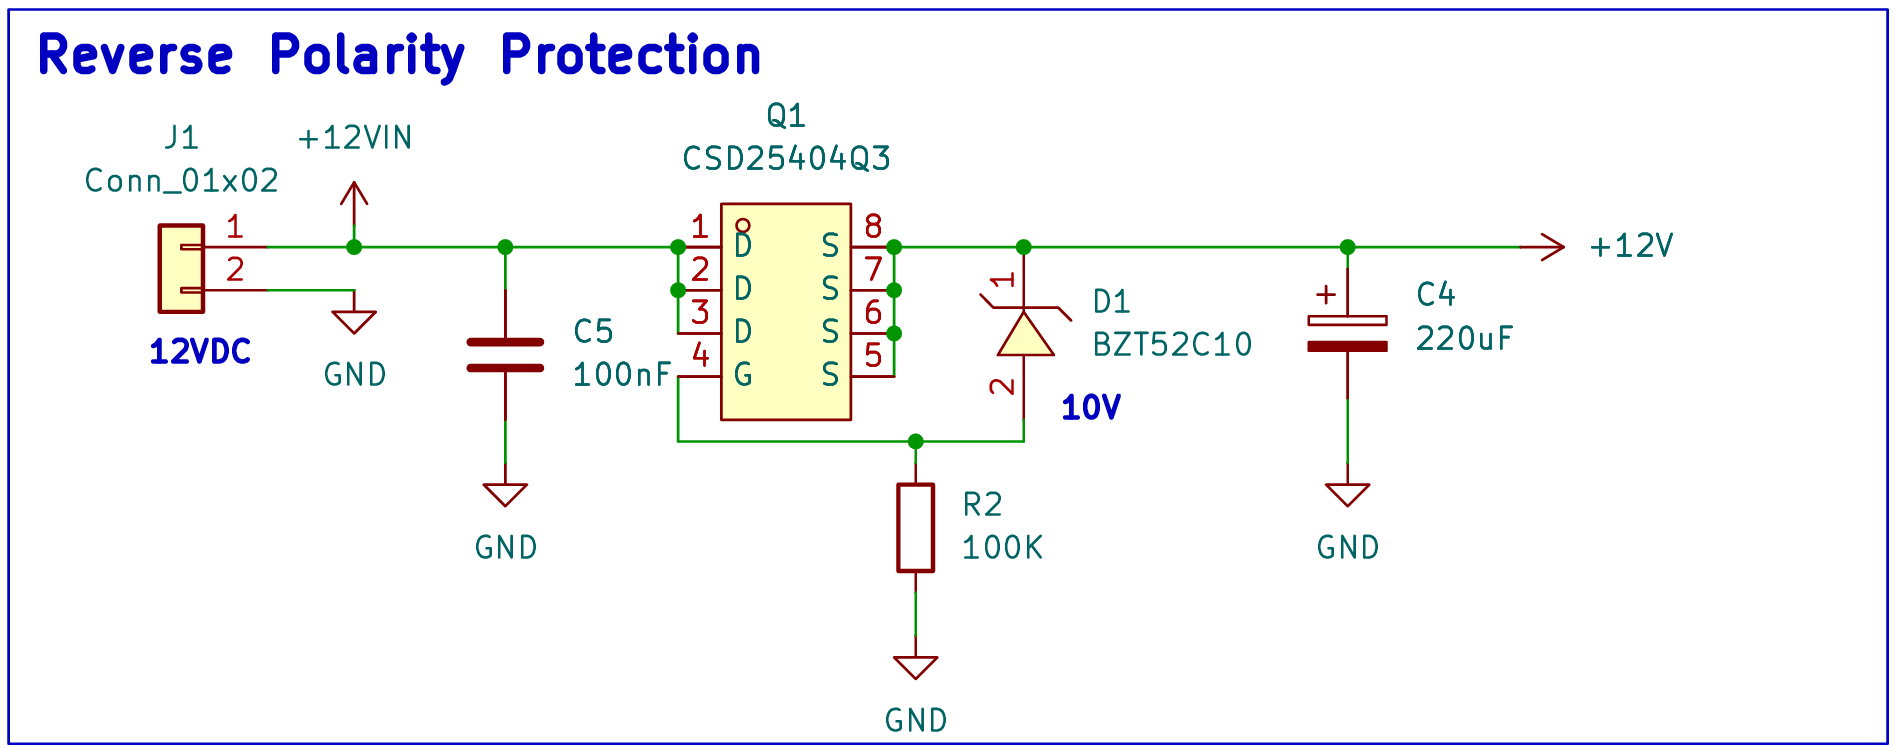
\includegraphics[width=0.9\linewidth]{figures/Reverse_polarity.png}
\caption{Mạch chống ngược cực dùng P-MOSFET CSD25404Q3}
\label{fig:sch_rpp}
\end{figure}

\paragraph{Điện áp ra của buck.} Với $V_{FB}=\SI{0.6}{\volt}$, $R_5=\SI{100}{\kilo\ohm}$ (FB lên +5V), $R_7=\SI{13.7}{\kilo\ohm}$ (FB xuống GND):
\begin{equation}
  V_{OUT}=0{,}6\left(1+\frac{100}{13{,}7}\right)=\SI{4.98}{\volt}.
\end{equation}
Cuộn cảm L2 = \SI{10}{\micro\henry} và hai tụ \SI{22}{\micro\farad} (C11, C12) ở ngõ ra được chọn theo bảng thiết kế trong datasheet LMR51420 (Table 9.2) cho $V_{OUT}=\SI{5}{\volt}$, $f_{SW}=\SI{500}{\kilo\hertz}$. Độ gợn dòng điện cuộn cảm (Inductance Current Ripple):
\begin{equation}
  \Delta I_L=\frac{V_{OUT}(V_{IN}-V_{OUT})}{V_{IN}\,L\,f_{SW}}=\frac{5\times(12-5)}{12\times10\cdot10^{-6}\times500\cdot10^{3}}\approx\SI{0.58}{\ampere}.
\end{equation}


\begin{figure}[H]
\centering
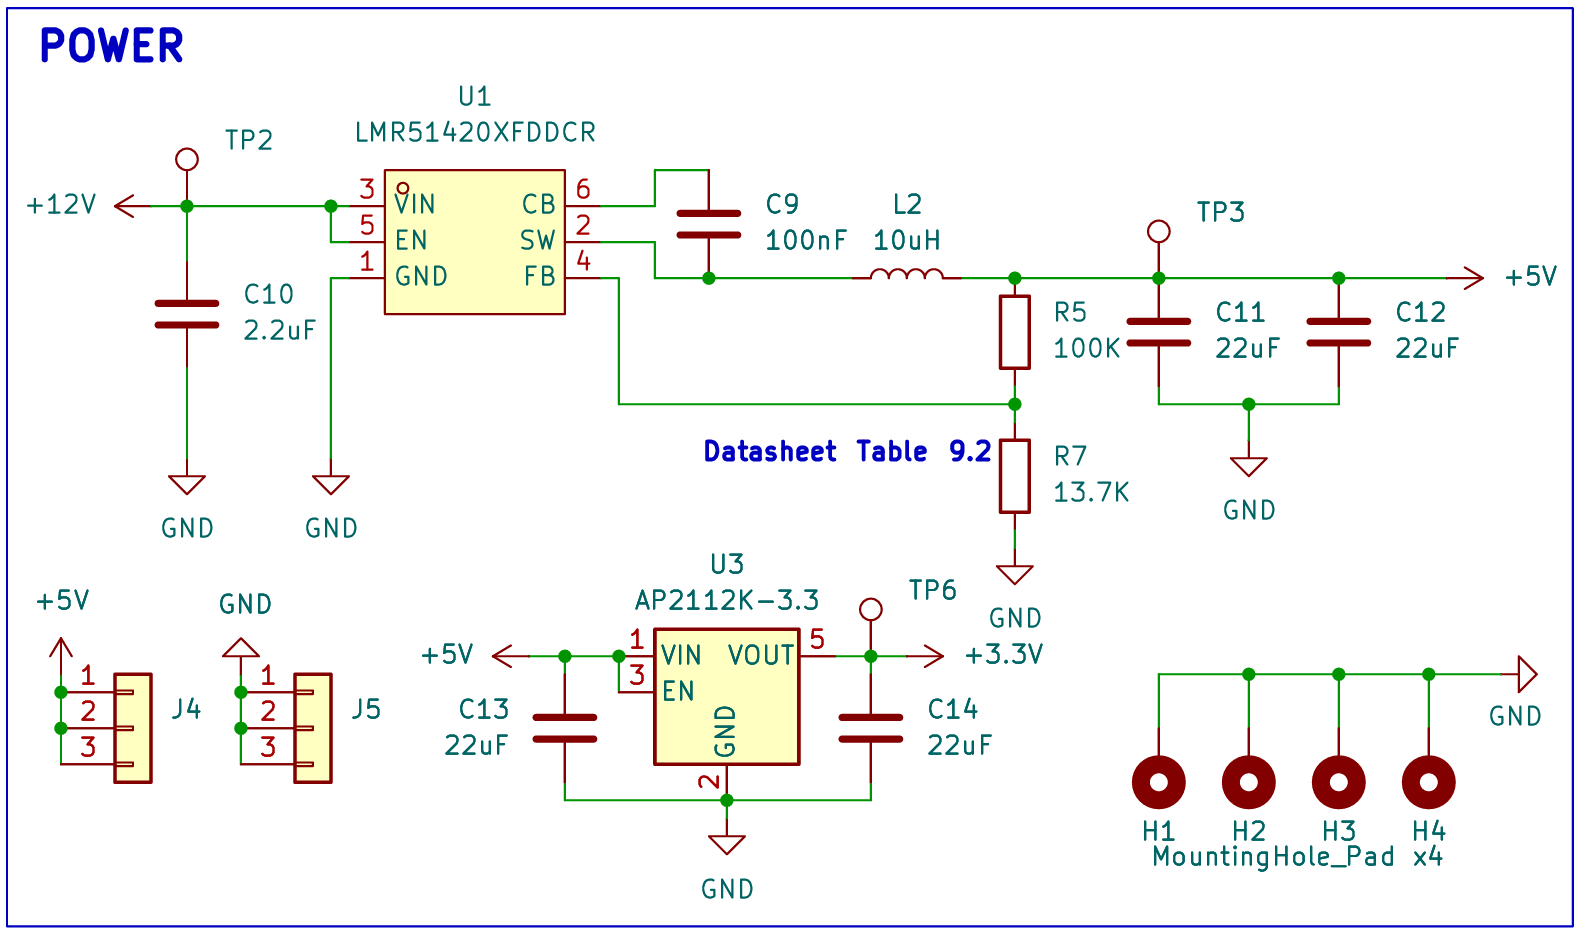
\includegraphics[width=0.9\linewidth]{figures/Power.png}
\caption{Khối nguồn: buck LMR51420 (\SI{12}{\volt}$\to$\SI{5}{\volt}) và LDO AP2112K (\SI{5}{\volt}$\to$\SI{3.3}{\volt})}
\label{fig:sch_power}
\end{figure}

\paragraph{Mạch dao động thạch anh.} Tụ tải C7, C8 = \SI{22}{\pico\farad}; với điện dung ký sinh $C_{stray}\approx\SI{5}{\pico\farad}$, điện dung tải tương đương $C_L=\frac{22\times22}{22+22}+5=\SI{16}{\pico\farad}$, phù hợp với thạch anh \SI{16}{\mega\hertz} thông dụng.

\paragraph{Nguồn tương tự AVCC.} Nguồn +5VA cấp cho AVCC được tách khỏi +5V qua cuộn cảm L1 (\SI{10}{\micro\henry}) / điện trở R1 (\SI{22}{\ohm}) và tụ C3, tạo bộ lọc thông thấp giảm nhiễu chuyển mạch từ buck và cầu H vào ADC. Chân AREF được thoát xuống đất qua C6 (\SI{10}{\nano\farad}).


\begin{figure}[H]
\centering
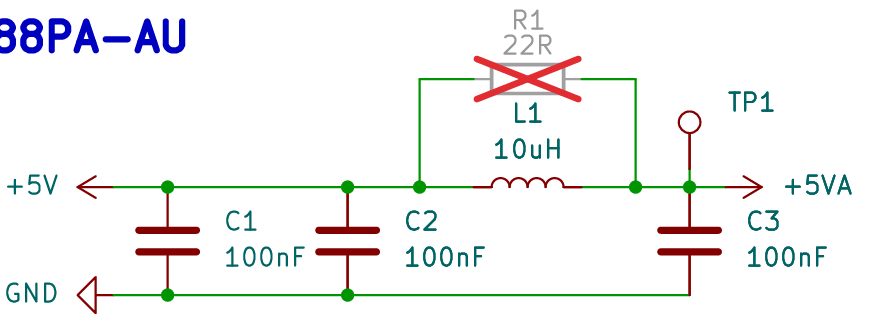
\includegraphics[width=0.6\linewidth]{figures/AVCC.png}
\caption{Bộ lọc nguồn tương tự +5VA cho AVCC}
\label{fig:sch_avcc}
\end{figure}

\paragraph{Nút nhấn.} Nút RUN (SW1) và STOP (SW2) nối lên +5V (tích cực mức cao), có điện trở kéo xuống \SI{10}{\kilo\ohm} và tụ \SI{100}{\nano\farad} tạo bộ lọc RC phần cứng với hằng số thời gian
\begin{equation}
  \tau=RC=10\cdot10^{3}\times100\cdot10^{-9}=\SI{1}{\milli\second},
\end{equation}
kết hợp với bộ chống dội phần mềm \SI{20}{\milli\second} trong firmware.


\begin{figure}[H]
\centering
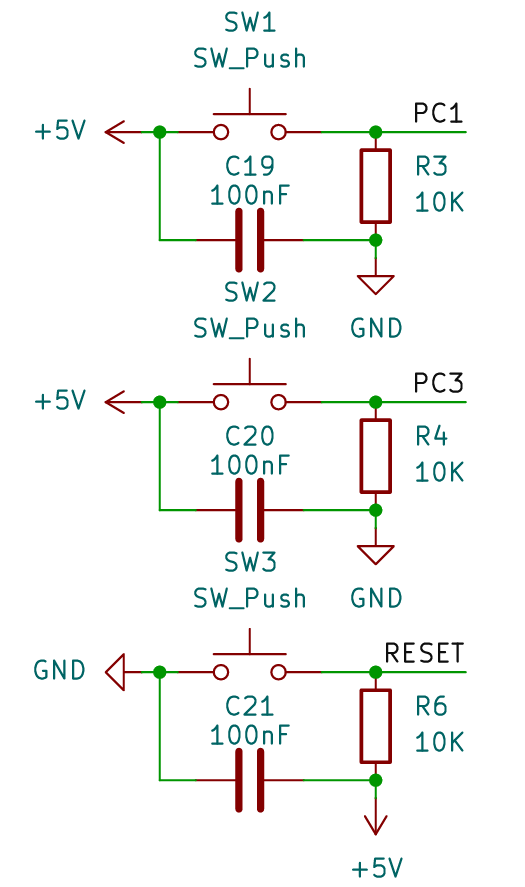
\includegraphics[width=0.35\linewidth]{figures/Button.png}
\caption{Mạch nút nhấn RUN (SW1), STOP (SW2) và RESET (SW3) với bộ lọc RC}
\label{fig:sch_button}
\end{figure}

\paragraph{LED trạng thái.} Mỗi LED được khóa bởi một MOSFET kênh N 2N7002 (Q2, Q3) ở phía thấp; cực cổng nối với chân GPIO qua \SI{22}{\ohm} và kéo xuống \SI{10}{\kilo\ohm} để LED tắt khi MCU đang reset. Dòng qua LED với trở hạn dòng \SI{10}{\kilo\ohm}:
\begin{equation}
  I_{LED}=\frac{V_{CC}-V_F}{R}\approx\frac{5-2}{10\cdot10^{3}}=\SI{0.3}{\milli\ampere},
\end{equation}
đủ sáng để báo hiệu với LED hiệu suất cao và giảm tải cho phần nguồn.

\begin{ghichu}[Vì sao R13 và R16 được đánh dấu DNP?]
Q2, Q3 dùng chung một footprint SOT-23 cho \textbf{hai phương án linh kiện}: MOSFET kênh N (2N7002) hoặc transistor BJT NPN (ví dụ MMBT3904). Hai loại này có sơ đồ chân tương thích trên vỏ SOT-23 (chân 1: G/B, chân 2: S/E, chân 3: D/C), nên có thể thay thế cho nhau mà không phải sửa PCB, tùy linh kiện sẵn có khi lắp ráp. R13 và R16 (\SI{10}{\kilo\ohm}, nối cực điều khiển xuống GND) chỉ cần thiết với một trong hai phương án, nên mặc định được đánh dấu \textbf{DNP} (\emph{Do Not Populate} -- không hàn) và chỉ hàn khi cần, đúng như ghi chú trên sơ đồ nguyên lý: \emph{``Solder R13 and R16 when Q2 and Q3 are MOSFETs''}.
\end{ghichu}


\begin{figure}[H]
\centering
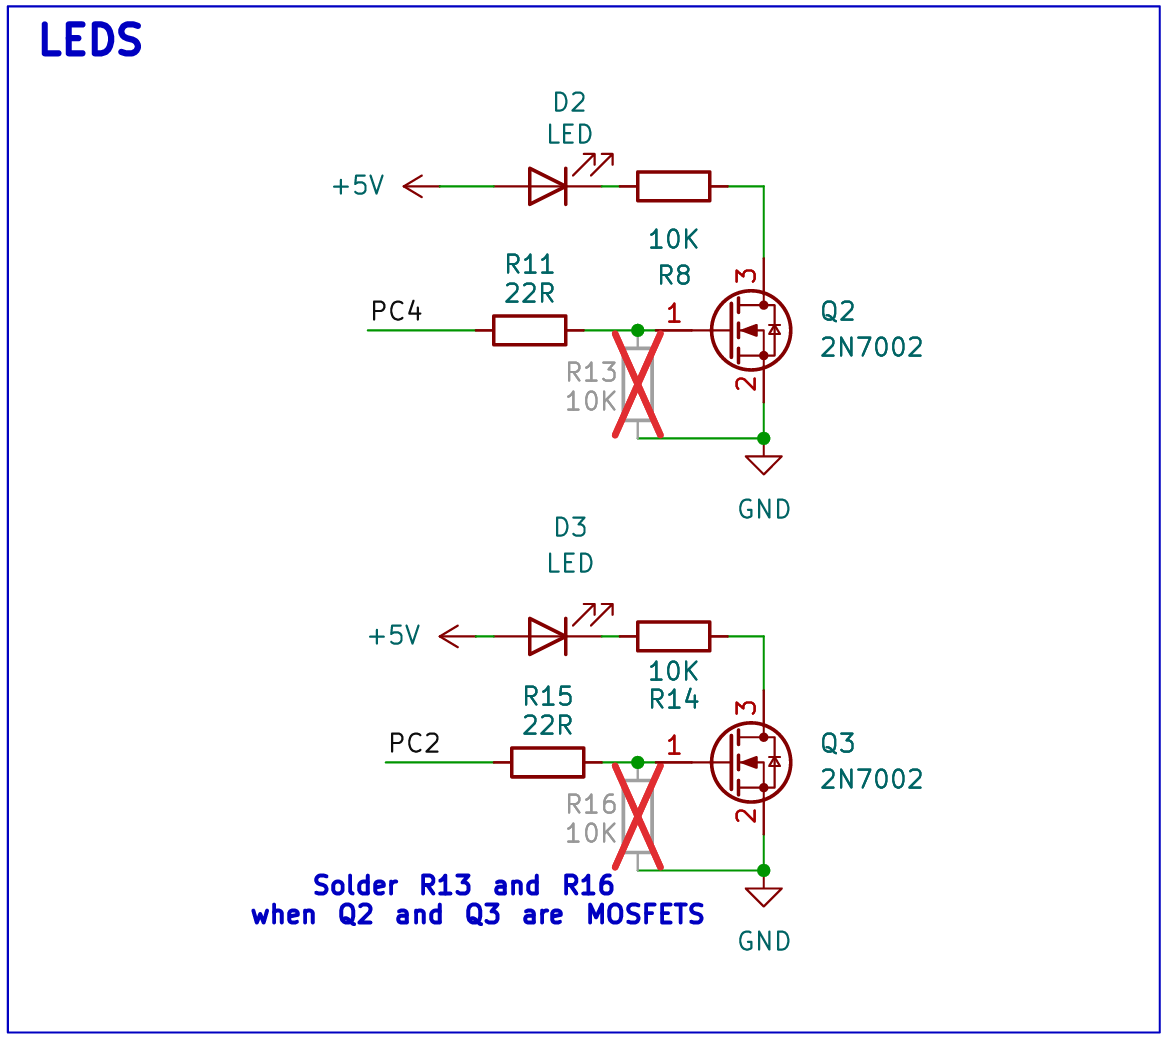
\includegraphics[width=0.7\linewidth]{figures/LEDs.png}
\caption{Mạch LED trạng thái khóa bằng MOSFET 2N7002}
\label{fig:sch_leds}
\end{figure}

\paragraph{Cổng nạp và Test point.} Đầu nối J6 (RESET, MOSI, MISO, SCK, GND) cho phép nạp ISP. Bảy Test point TP1--TP7 được đặt tại các nút quan trọng: +5VA, +12V, +5V, ENC\_A, ENC\_B, +3.3V và OE -- phục vụ trực tiếp việc đo kiểm ở Chương~\ref{ch:lapdat}.

\section{Thiết kế mạch in (PCB)}

\subsection{Thông số bo mạch}
\begin{table}[H]
\centering\small
\caption{Thông số chế tạo PCB}
\label{tab:pcbspec}
\begin{tabular}{@{}ll@{}}
\toprule
\textbf{Thông số} & \textbf{Giá trị}\\
\midrule
Kích thước & 80\,$\times$\,60\,mm\\
Số lớp đồng & 2 (F.Cu, B.Cu)\\
Độ dày bo & \SI{1.6}{\milli\metre} FR-4\\
Độ rộng đường tín hiệu & \SIrange{0.2}{0.3}{\milli\metre}\\
Độ rộng đường nguồn & \SI{0.5}{\milli\metre} và đổ đồng (copper pour)\\
Số via & 280 (bao gồm via khâu mặt đất và via tản nhiệt)\\
Lỗ bắt vít & 4 $\times$ M3, có pad nối GND\\
Gia công & Đặt sản xuất tại JLCPCB từ tệp Gerber xuất từ KiCad\\
\bottomrule
\end{tabular}
\end{table}

\subsection{Bố trí linh kiện (placement)}
Bo mạch được chia thành các vùng chức năng rõ ràng nhằm tách biệt dòng công suất khỏi tín hiệu nhạy cảm:
\begin{itemize}
  \item \textbf{Vùng nguồn} (cạnh trái): đầu vào J1, MOSFET chống ngược cực Q1, buck U1, LDO U3 và các tụ bulk. Đầu nối nguồn đặt ở mép bo để dễ đấu dây (Hình~\ref{fig:place_power}).
  \item \textbf{Vùng công suất} (góc trên bên phải): DRV8220 (U5), jumper chọn chế độ JP1 và domino động cơ M1 ở mép phải -- đường dòng động cơ ngắn và nằm xa vùng tương tự (Hình~\ref{fig:place_motor}).
  \item \textbf{Vùng vi điều khiển} (trung tâm): ATmega88PA (U2) với thạch anh Y1 đặt sát chân XTAL1/\allowbreak XTAL2, các tụ thoát \SI{100}{\nano\farad} đặt sát từng chân cấp nguồn; cổng nạp J6 ngay phía trên MCU (Hình~\ref{fig:place_mcu}).
  \item \textbf{Vùng giao diện}: header màn hình J2 và IC chuyển mức U4 ở bên trái -- màn hình cắm chồng lên bo; chiết áp RV1, nút RUN/STOP/RESET và LED xếp dọc cạnh dưới để người dùng thao tác; đầu JST encoder J7 và UART J3 gom về cạnh phải (Hình~\ref{fig:place_ui}).
\end{itemize}

\begin{figure}[H]
\centering
\begin{subfigure}{0.65\linewidth}\centering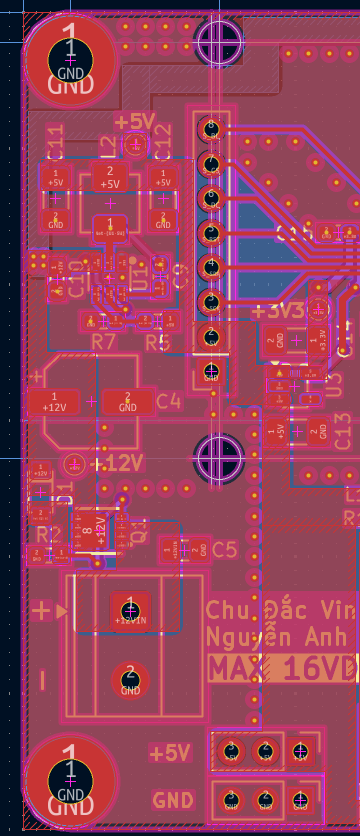
\includegraphics[angle=90,width=\linewidth]{figures/Power_Layout.png}\caption{Layout}\end{subfigure}

\vspace{0.5em}
\begin{subfigure}{0.65\linewidth}\centering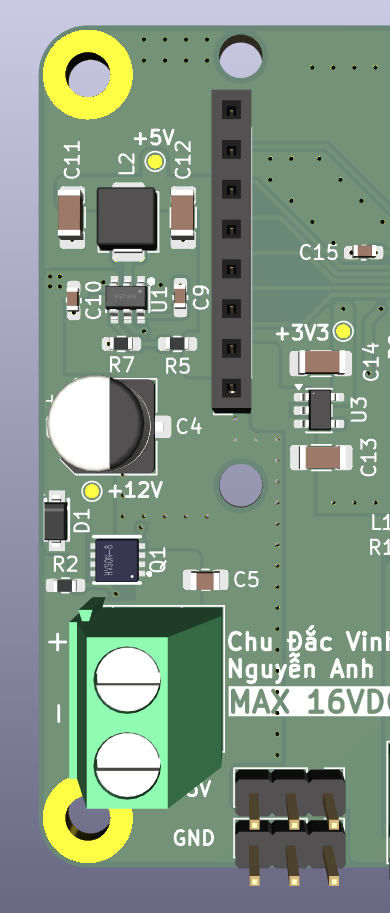
\includegraphics[angle=90,width=\linewidth]{figures/Power_3D.png}\caption{Ảnh 3D}\end{subfigure}
\caption{Bố trí linh kiện vùng nguồn}
\label{fig:place_power}
\end{figure}

\begin{figure}[H]
\centering
\begin{subfigure}{0.65\linewidth}\centering\hinh[\linewidth]{figures/Motor_Driver_Layout.png}{Layout vùng công suất (cầu H DRV8220)}\caption{Layout}\end{subfigure}

\vspace{0.5em}
\begin{subfigure}{0.65\linewidth}\centering\hinh[\linewidth]{figures/Motor_Driver_3D.png}{Ảnh 3D vùng công suất (cầu H DRV8220)}\caption{Ảnh 3D}\end{subfigure}
\caption{Bố trí linh kiện vùng công suất (cầu H DRV8220)}
\label{fig:place_motor}
\end{figure}

\begin{figure}[H]
\centering
\begin{subfigure}{0.49\linewidth}\centering\hinh[\linewidth]{figures/MCU_Layout.png}{Layout vùng vi điều khiển}\caption{Layout}\end{subfigure}
\hfill
\begin{subfigure}{0.49\linewidth}\centering\hinh[\linewidth]{figures/MCU_3D.png}{Ảnh 3D vùng vi điều khiển}\caption{Ảnh 3D}\end{subfigure}
\caption{Bố trí linh kiện vùng vi điều khiển}
\label{fig:place_mcu}
\end{figure}

\begin{figure}[H]
\centering
\begin{subfigure}{0.65\linewidth}\centering\hinh[\linewidth]{figures/UI_Layout.png}{Layout vùng giao diện người dùng}\caption{Layout}\end{subfigure}

\vspace{0.5em}
\begin{subfigure}{0.65\linewidth}\centering\hinh[\linewidth]{figures/UI_3D.png}{Ảnh 3D vùng giao diện người dùng}\caption{Ảnh 3D}\end{subfigure}
\caption{Bố trí linh kiện vùng giao diện người dùng}
\label{fig:place_ui}
\end{figure}

\subsection{Đi dây (routing)}
\begin{itemize}
  \item \textbf{Vòng chuyển mạch buck} (VIN -- tụ vào -- chân SW -- cuộn cảm -- tụ ra -- GND) được giữ ngắn và nhỏ nhất có thể để giảm bức xạ nhiễu điện từ, tụ vào C10 đặt sát chân VIN/GND của U1.
  \item \textbf{Đường dòng động cơ} (VM, OUT1, OUT2) dùng đường rộng \SI{0.5}{\milli\metre} và vùng đổ đồng; pad tản nhiệt (exposed pad) của DRV8220 được khâu xuống mặt dưới bằng nhiều via.
  \item \textbf{Mặt đất và vùng đồng nguồn}: GND được đổ đồng trên cả hai lớp; các vùng đồng riêng cho +12V, +5V, +5VA, +3.3V và OUT1/OUT2 nằm ở lớp trên. Phần lớn đường tín hiệu đi ở lớp trên (210/250 đoạn dây) để mặt đất lớp dưới ít bị cắt; các via khâu (stitching via) nối đồng GND hai lớp.
  \item \textbf{Đường tín hiệu nhạy}: đường encoder và ADC chiết áp đi xa vùng chuyển mạch; đường SPI tới TFT đi ngắn qua TXB0106.
\end{itemize}

\begin{figure}[H]
\centering
\begin{subfigure}{0.49\linewidth}\centering\hinh[\linewidth]{figures/Layout_Front.png}{Layout lớp trên}\caption{Lớp trên (F.Cu)}\end{subfigure}
\hfill
\begin{subfigure}{0.49\linewidth}\centering\hinh[\linewidth]{figures/Layout_Back.png}{Layout lớp dưới}\caption{Lớp dưới (B.Cu)}\end{subfigure}
\caption{Layout mạch in \proj}
\label{fig:layout}
\end{figure}

\subsection{Kiểm tra và xuất tệp sản xuất}
Trước khi đặt gia công, thiết kế được kiểm tra bằng ERC (Electrical Rules Check) cho sơ đồ nguyên lý và DRC (Design Rules Check) cho PCB theo năng lực công nghệ của nhà sản xuất (đường/khoảng cách tối thiểu \SI{0.15}{\milli\metre}, lỗ khoan tối thiểu \SI{0.3}{\milli\metre}). Bộ tệp sản xuất gồm Gerber các lớp đồng, mặt nạ hàn, lụa, kem hàn, đường viền bo (Edge.Cuts) và tệp khoan Excellon (\texttt{.drl}).

Trước khi gửi đi gia công, bộ tệp Gerber được mở lại bằng trình xem Gerber (Gerber Viewer) để kiểm tra lần cuối: các lớp đồng, mặt nạ hàn, lụa và lỗ khoan phải chồng khớp nhau, đường viền bo khép kín và không có lớp nào bị thiếu hoặc lệch so với thiết kế (Hình~\ref{fig:gerber}).

\begin{figure}[H]
\centering
\hinh[0.85\linewidth]{figures/Gerber_Viewer.png}{Kiểm tra bộ tệp Gerber trên trình xem Gerber}
\caption{Kiểm tra bộ tệp sản xuất trên Gerber Viewer}
\label{fig:gerber}
\end{figure}

\subsubsection{Dụng cụ hàn linh kiện}
Sau khi nhận bo mạch trần, linh kiện được hàn thủ công tại chỗ. Do phần lớn linh kiện là loại dán bề mặt (SMD) với bước chân nhỏ, phương pháp chính là quét kem hàn lên pad rồi dùng khí nóng để nung chảy (hot-air reflow); mỏ hàn chỉ dùng cho linh kiện xuyên lỗ và sửa mối hàn. Các dụng cụ được sử dụng được liệt kê ở Bảng~\ref{tab:solder_equipment} và Hình~\ref{fig:solder_equipment}.

\begin{table}[H]
\centering
\caption{Dụng cụ hàn và lắp ráp linh kiện}
\label{tab:solder_equipment}
\begin{tabularx}{\linewidth}{|l|X|}
\hline
\textbf{Dụng cụ} & \textbf{Công dụng} \\
\hline
Kem hàn Relife RL-403S & Kem hàn dạng ống tiêm \SI{10}{cc}, nhiệt độ nóng chảy \SI{183}{\celsius}; được bơm trực tiếp lên từng pad SMD trước khi đặt linh kiện. \\
\hline
Súng bơm kem hàn Relife RL-062A & Gắn với ống kem hàn RL-403S, giúp định lượng và đưa kem hàn lên pad chính xác, đều tay. \\
\hline
Trạm khò hàn AIFEN 868D & Thổi khí nóng để nung chảy kem hàn (reflow) cho các linh kiện SMD như IC, điện trở, tụ điện; đồng thời dùng để tháo linh kiện khi cần sửa. \\
\hline
Trạm hàn SUNSHINE S3 & Mỏ hàn dùng để hàn linh kiện xuyên lỗ (header, domino, đầu nối), sửa mối hàn thiếu thiếc hoặc bị dính chân (bridge). \\
\hline
Nhíp Relife SA-11 & Gắp, đặt và căn chỉnh linh kiện SMD lên vị trí trước và trong khi khò. \\
\hline
\end{tabularx}
\end{table}

Quy trình hàn được thực hiện theo thứ tự: (1) bơm kem hàn lên các pad bằng súng RL-062A; (2) dùng nhíp SA-11 đặt linh kiện SMD vào đúng vị trí và chiều; (3) khò bằng trạm AIFEN 868D tới khi kem hàn chảy và linh kiện tự căn chỉnh vào pad nhờ sức căng bề mặt; (4) hàn các linh kiện xuyên lỗ và kiểm tra, sửa mối hàn bằng trạm hàn SUNSHINE S3.

\begin{figure}[H]
\centering
\hinh[0.8\linewidth]{figures/solder_equipment.png}{Ảnh các dụng cụ hàn linh kiện}
\caption{Các dụng cụ dùng để hàn linh kiện}
\label{fig:solder_equipment}
\end{figure}

\begin{figure}[H]
\centering
\hinh[0.7\linewidth]{figures/pcb_thucte.jpg}{Ảnh chụp bo mạch thực tế sau khi hàn linh kiện}
\caption{Bo mạch \proj{} sau khi lắp ráp}
\label{fig:pcbthucte}
\end{figure}

%%!TEX root = ./main.tex
%!TEX program = xelatex
% =====================================================================
%  03 - CẤU TRÚC FIRMWARE
% =====================================================================
\chapter{Cấu trúc firmware}
\label{ch:firmware}

\section{Nguyên tắc thiết kế}
Firmware của \proj{} được viết theo phong cách \textbf{bare-metal}: mọi ngoại vi (Timer, ADC, SPI, USART, ngắt ngoài) đều được cấu hình bằng cách ghi trực tiếp vào thanh ghi, các trình phục vụ ngắt (ISR) được viết tay. Framework Arduino chỉ được dùng cho hai việc: hàm \texttt{millis()} (dựa trên Timer0) và cặp điểm vào \texttt{setup()}/\texttt{loop()} dưới môi trường PlatformIO. Cách tiếp cận này xuất phát từ ba lý do:
\begin{enumerate}
  \item \textbf{Bộ nhớ hạn chế:} ATmega88PA chỉ có 8\,KB Flash; riêng thư viện đồ họa Adafruit cho ST7735 đã vượt quá dung lượng này. Nhóm tự viết driver \texttt{st7735\_mini} chỉ hiển thị chữ để vừa bộ nhớ.
  \item \textbf{Xung đột chân phần cứng:} các chân PWM phần cứng của Timer2 trùng với MOSI (PB3/OC2A) và ENC\_B (PD3/OC2B), nên PWM phải được tạo bằng phần mềm (mục~\ref{sec:swpwm}).
  \item \textbf{Mục tiêu học tập:} làm chủ cơ chế ngắt, timer và thanh ghi -- nội dung cốt lõi của học phần.
\end{enumerate}
Mọi thông số có thể tinh chỉnh (chân, tần số, hệ số PID, giao diện\ldots) được tập trung trong \textbf{một tệp duy nhất} \texttt{config.h}, giúp \proj{} thích ứng với động cơ và encoder khác mà không phải sửa mã nguồn thư viện.

\section{Phân lớp firmware (firmware stack-up)}

Firmware được tổ chức thành các lớp chồng lên nhau (Hình~\ref{fig:stackup}); mỗi lớp chỉ gọi xuống lớp ngay bên dưới, giúp mã dễ đọc, dễ kiểm thử và dễ chuyển sang vi điều khiển khác.

\begin{figure}[H]
\centering
\resizebox{\linewidth}{!}{%
\begin{tikzpicture}[
  layer/.style={draw=blk,thick,minimum height=11mm,align=center,font=\small},
  mod/.style={draw=blk,fill=white,rounded corners=2pt,minimum height=8mm,align=center,font=\scriptsize,inner sep=2pt}]
  \def\W{12}
  % lớp
  \node[layer,fill=hustred!15,minimum width=\W cm] (l5) at (0,5.2) {};
  \node[layer,fill=swfill,minimum width=\W cm] (l4) at (0,3.9) {};
  \node[layer,fill=blkfill,minimum width=\W cm] (l3) at (0,2.6) {};
  \node[layer,fill=blkfill!50,minimum width=\W cm,minimum height=14mm] (l2) at (0,1.15) {};
  \node[layer,fill=iofill,minimum width=\W cm] (l1) at (0,-0.3) {};
  \node[layer,fill=gray!20,minimum width=\W cm] (l0) at (0,-1.6) {};
  % nhãn lớp
  \foreach \l/\t in {l5/Điểm vào,l4/Ứng dụng,l3/Điều khiển,l2/Driver ngoại vi,l1/HAL / thanh ghi AVR,l0/Phần cứng}
     \node[anchor=east,font=\small\bfseries,text width=2.6cm,align=right] at ([xshift=-2mm]\l.west) {\t};
  % module
  \node[mod] at (0,5.2) {main.cpp: setup() $\to$ app\_init(), loop() $\to$ app\_update()};
  \node[mod,text width=10.5cm] at (0,3.9) {app.cpp -- máy trạng thái STOP/RUN/SELECT, chọn chế độ, LED, ánh xạ tốc độ đặt, hiển thị};
  \node[mod,text width=10.5cm] at (0,2.6) {motion.c -- PID dấu phẩy tĩnh Q8 + feed-forward + ramp + anti-windup};
  \node[mod] at (-4.6,1.15) {motor.c\\PWM mềm};
  \node[mod] at (-2.6,1.15) {encoder\_mini\\giải mã $\times$4};
  \node[mod] at (-0.65,1.15) {st7735\_mini\\TFT SPI};
  \node[mod] at (1.2,1.15) {uart.c\\ring buffer};
  \node[mod] at (2.85,1.15) {button.c\\chống dội};
  \node[mod] at (4.5,1.15) {adc.c\\10-bit};
  \node[mod,text width=10.5cm] at (0,-0.3) {<avr/io.h>, <avr/interrupt.h>, ISR, Timer0 (millis), Timer1, Timer2, SPI, USART0, ADC, GPIO};
  \node[font=\small] at (0,-1.6) {ATmega88PA \quad DRV8220 \quad Encoder \quad TFT \quad Nút/LED \quad Chiết áp};
  % config.h
  \node[draw=hustred,very thick,fill=hustred!8,minimum width=7.6cm,minimum height=0.9cm,align=center,font=\small,rotate=90] at (6.65,1.8) {\texttt{config.h} -- toàn bộ thông số cấu hình};
\end{tikzpicture}}
\caption{Phân lớp firmware \proj}
\label{fig:stackup}
\end{figure}

\begin{table}[H]
\centering\small
\caption{Các module firmware}
\label{tab:modules}
\begin{tabularx}{\linewidth}{@{}l>{\raggedright\arraybackslash}X@{}}
\toprule
\textbf{Tệp} & \textbf{Chức năng}\\
\midrule
\texttt{main.cpp} & Điểm vào, chỉ gọi \texttt{app\_init()} và \texttt{app\_update()}\\
\texttt{app.cpp/.h} & Lớp ứng dụng: máy trạng thái, chọn chế độ, LED, cập nhật màn hình (hiện thực đặc tả logic nút nhấn)\\
\texttt{config.h} & Tệp cấu hình duy nhất: chân, TFT, ADC, encoder, động cơ, hệ số PID, thời gian nút nhấn, bố cục giao diện\\
\texttt{motion.c/.h} & Bộ điều khiển vận tốc PID dấu phẩy tĩnh Q8, có bù thuận, giới hạn gia tốc, chống bão hòa tích phân, lọc khâu D\\
\texttt{motor.c/.h} & Driver DRV8220, PWM mềm bằng ngắt Timer2 (không đụng tới Timer0/\texttt{millis()})\\
\texttt{encoder\_mini.cpp/.h} & Giải mã encoder cầu phương $\times4$, bộ lọc số kiểu STM32 (Timer1), tính vận tốc và RPM\\
\texttt{button.c/.h} & Nút nhấn có chống dội, phát hiện nhấn ngắn / nhấn giữ\\
\texttt{uart.c/.h} & Nhận UART bằng ngắt, bộ đệm vòng 32 byte, bộ phân tích số nguyên ASCII\\
\texttt{adc.c/.h} & Driver ADC 10-bit tối giản\\
\texttt{st7735\_mini.c/.h} & Driver TFT ST7735 rút gọn, chỉ hiển thị chữ, font lưu trong Flash (PROGMEM)\\
\bottomrule
\end{tabularx}
\end{table}

\section{Tài nguyên phần cứng và ngắt}

\begin{table}[H]
\centering\small
\caption{Phân bổ timer và ngắt}
\label{tab:interrupts}
\begin{tabularx}{\linewidth}{@{}lll>{\raggedright\arraybackslash}X@{}}
\toprule
\textbf{Ngoại vi} & \textbf{Vector ngắt} & \textbf{Tần suất} & \textbf{Nhiệm vụ}\\
\midrule
Timer0 & \texttt{TIMER0\_OVF} & \SI{976}{\hertz} & \texttt{millis()} của Arduino -- cơ sở thời gian toàn hệ thống\\
Timer1 (CTC) & \texttt{TIMER1\_COMPA} & \SI{80}{\kilo\hertz} & Lấy mẫu và lọc số kênh A/B encoder, đếm xung\\
Timer2 (Fast PWM) & \texttt{TIMER2\_OVF} & \SI{1953}{\hertz} & Bắt đầu chu kỳ PWM: đặt mức cao các chân đang băm xung\\
 & \texttt{TIMER2\_COMPA/B} & \SI{1953}{\hertz} & Kết thúc độ rộng xung trên IN1 (PD5) / IN2 (PD6)\\
USART0 & \texttt{USART\_RX} & theo dữ liệu & Đưa byte nhận được vào bộ đệm vòng\\
SPI & -- (polling) & -- & Gửi dữ liệu tới TFT tại \SI{8}{\mega\hertz}\\
ADC & -- (polling) & -- & Đọc chiết áp, xung nhịp ADC \SI{125}{\kilo\hertz}\\
\bottomrule
\end{tabularx}
\end{table}

Với cấu hình mặc định, ISR của Timer1 chạy mỗi $16\,000\,000/80\,000=200$ chu kỳ máy. Nếu mỗi lần thực thi tốn khoảng 60--80 chu kỳ (bao gồm lưu/khôi phục ngữ cảnh), riêng bộ lọc encoder đã chiếm khoảng 30--40\,\% thời gian CPU. Đây là cái giá của việc lọc nhiễu bằng phần mềm trên một vi điều khiển không có khối giải mã encoder phần cứng, và là một trong những lý do nâng cấp lên \projpro{} (Chương~\ref{ch:ketluan}).

\section{Logic hoạt động}

\subsection{Máy trạng thái}
Hệ thống có ba trạng thái người dùng nhìn thấy: \textbf{STOP}, \textbf{RUN} và \textbf{SELECT} (chọn chế độ), cùng hai chế độ đặt tốc độ: \textbf{POTENTIOMETER} và \textbf{UART}. Biến toàn cục \texttt{running} bằng 1 khi hệ thống đang chạy và bằng 0 trong các trường hợp còn lại.

\begin{figure}[H]
\centering
\begin{tikzpicture}[
  state/.style={circle,draw=blk,very thick,fill=blkfill,minimum size=22mm,align=center,font=\small\bfseries},
  ar/.style={-{Stealth[length=3mm]},thick},
  lb/.style={font=\scriptsize,align=center,fill=white,inner sep=1pt}]
  \node[state,fill=hustred!15,draw=hustred] (stop) at (0,0) {STOP\\[-2pt]\tiny LED STOP};
  \node[state,fill=iofill,draw=green!40!black] (run) at (6.5,0) {RUN\\[-2pt]\tiny LED RUN};
  \node[state,fill=swfill,draw=orange!80!black] (sel) at (0,-4.6) {SELECT\\[-2pt]\tiny LED STOP};
  \draw[ar] (-2.3,1.6) node[above,font=\scriptsize]{Cấp nguồn} -- (stop);
  \draw[ar] (stop) to[bend left=18] node[lb,above]{RUN nhấn ngắn\\ \texttt{motor\_enable(1)}, \texttt{motion\_start()}} (run);
  \draw[ar] (run) to[bend left=18] node[lb,below]{STOP nhấn\\ \texttt{motion\_stop()}, nSLEEP = 0} (stop);
  \draw[ar] (stop) to[bend right=25] node[lb,left]{RUN giữ 2\,s} (sel);
  \draw[ar] (sel) to[bend right=25] node[lb,right]{RUN giữ 2\,s\\(xác nhận chế độ)\\hoặc STOP (hủy)} (stop);
  \draw[ar] (sel) edge[loop below,looseness=5] node[lb,below]{RUN nhấn ngắn: đổi POT $\leftrightarrow$ UART} (sel);
  \draw[ar] (run) edge[loop right,looseness=5] node[lb,right]{RUN: bỏ qua} (run);
\end{tikzpicture}
\caption{Máy trạng thái của \proj}
\label{fig:fsm}
\end{figure}

\begin{table}[H]
\centering\small
\caption{Bảng logic nút nhấn}
\label{tab:buttonlogic}
\begin{tabularx}{\linewidth}{@{}llll>{\raggedright\arraybackslash}X@{}}
\toprule
\textbf{Nút} & \textbf{TT hiện tại} & \textbf{Thao tác} & \textbf{TT mới} & \textbf{Kết quả}\\
\midrule
STOP & bất kỳ & Nhấn & STOP & Kéo PD4 (nSLEEP) xuống thấp, reset PID, hủy chọn chế độ dang dở\\
RUN & STOP & Nhấn ngắn & RUN & Chạy ở chế độ hiện hành\\
RUN & STOP & Giữ $\approx$\SI{2}{\second} & SELECT & Vào chế độ chọn\\
RUN & SELECT & Nhấn ngắn & SELECT & Đổi giữa POTENTIOMETER và UART\\
RUN & SELECT & Giữ $\approx$\SI{2}{\second} & STOP & Xác nhận chế độ đang hiển thị\\
RUN & RUN & bất kỳ & RUN & Bỏ qua\\
\bottomrule
\end{tabularx}
\end{table}

Nút STOP luôn có \textbf{quyền ưu tiên cao nhất}: trong hàm \texttt{handleButtons()}, sự kiện của nút STOP được xử lý trước và kết thúc hàm ngay lập tức, đảm bảo động cơ luôn có thể được dừng an toàn bất kể hệ thống đang ở trạng thái nào.

\subsection{Vòng lặp chính (super-loop)}
\proj{} không dùng hệ điều hành thời gian thực mà dùng kiến trúc \emph{super-loop} kết hợp ngắt: các tác vụ có yêu cầu thời gian khắt khe (đếm encoder, PWM, nhận UART) chạy trong ISR; các tác vụ còn lại chạy tuần tự trong \texttt{app\_update()} và tự định thời bằng \texttt{millis()} (không dùng \texttt{delay()} chặn).

\begin{figure}[H]
\centering
\begin{tikzpicture}[
  node distance=5mm,
  proc/.style={draw=blk,thick,fill=blkfill,rounded corners=2pt,minimum width=56mm,minimum height=8mm,align=center,font=\small},
  dec/.style={draw=blk,thick,fill=swfill,diamond,aspect=2.6,inner sep=1pt,align=center,font=\scriptsize},
  term/.style={draw=blk,thick,fill=hustred!15,rounded rectangle,minimum width=30mm,minimum height=8mm,font=\small},
  ar/.style={-{Stealth[length=2.5mm]},thick}]
  \node[term] (s) {Bắt đầu};
  \node[proc,below=of s] (init) {\texttt{app\_init()}: GPIO, TFT, ADC, UART,\\encoder, motor, PID $\to$ trạng thái STOP};
  \node[proc,below=7mm of init] (btn) {\texttt{handleButtons()}: cập nhật máy trạng thái};
  \node[proc,below=of btn] (vel) {\texttt{updateVelocity()}: mỗi \SI{50}{\milli\second} tính RPM từ encoder};
  \node[proc,below=of vel] (tgt) {\texttt{updateTarget()}: đọc chiết áp hoặc UART\\$\to$ tốc độ đặt (chỉ khi RUN)};
  \node[dec,below=of tgt] (dt) {Đủ \SI{50}{\milli\second}\\và đang RUN?};
  \node[proc,below=6mm of dt] (pid) {\texttt{motion\_update()}: ramp $\to$ PID + FF\\$\to$ \texttt{motor\_set(duty)}};
  \node[proc,below=of pid] (disp) {\texttt{drawMode/State()}; mỗi \SI{100}{\milli\second} \texttt{drawVelocity()}};
  \draw[ar] (s) -- (init); \draw[ar] (init) -- (btn); \draw[ar] (btn) -- (vel); \draw[ar] (vel) -- (tgt);
  \draw[ar] (tgt) -- (dt); \draw[ar] (dt) -- node[right,font=\scriptsize]{Đúng} (pid); \draw[ar] (pid) -- (disp);
  \draw[ar] (dt.east) -- ++(2.4,0) node[above,font=\scriptsize,pos=0.4]{Sai} |- (disp.east);
  \draw[ar] (disp.west) -- ++(-1.2,0) |- (btn.west);
  % ISR song song
  \node[draw=hustred,dashed,thick,fill=hustred!5,align=left,font=\scriptsize,right=16mm of vel,text width=40mm] (isr) {\textbf{Chạy song song bằng ngắt}\\[2pt]
   \texttt{TIMER1\_COMPA}: lọc + đếm encoder\\ \texttt{TIMER2\_OVF/COMPA/COMPB}: PWM\\ \texttt{USART\_RX}: bộ đệm vòng\\ \texttt{TIMER0\_OVF}: \texttt{millis()}};
\end{tikzpicture}
\caption{Lưu đồ vòng lặp chính}
\label{fig:mainloop}
\end{figure}

\section{Sơ đồ khối firmware và luồng dữ liệu}

Hình~\ref{fig:fwblock} thể hiện luồng dữ liệu của vòng điều khiển từ đầu vào người dùng tới động cơ và ngược lại.

\begin{figure}[H]
\centering
\resizebox{\linewidth}{!}{%
\begin{tikzpicture}[
  node distance=6mm and 7mm,
  b/.style={draw=blk,thick,fill=blkfill,rounded corners=2pt,minimum height=12mm,align=center,font=\small},
  hw/.style={draw,dashed,rounded corners=2pt,minimum height=12mm,align=center,font=\small},
  sum/.style={circle,draw=blk,thick,minimum size=6mm,inner sep=0},
  ar/.style={-{Stealth[length=2.5mm]},thick},
  lb/.style={font=\scriptsize,above}]
  \node[hw] (pot) {Chiết áp\\ADC0};
  \node[hw,below=of pot] (ua) {UART\\``-255..255\textbackslash n''};
  \node[b,right=of pot,yshift=-9mm] (map) {Ánh xạ\\$[-255,255]$\\$\to\pm2700$ rpm};
  \node[b,right=of map] (ramp) {Giới hạn\\gia tốc\\6000 rpm/s};
  \node[sum,right=of ramp] (s1) {};
  \node[b,right=of s1] (pid) {PID Q8\\$K_p, K_i, K_d$};
  \node[b,above=of pid] (ff) {Bù thuận\\$K_{ff}\cdot r$};
  \node[sum,right=of pid] (s2) {};
  \node[b,right=of s2] (sat) {Bão hòa\\$\pm255$ +\\anti-windup};
  \node[b,right=of sat] (pwm) {PWM mềm\\Timer2\\1,95\,kHz};
  \node[hw,right=of pwm] (drv) {DRV8220\\+ động cơ};
  \node[b,below=14mm of sat] (enc) {Giải mã $\times4$\\lọc số\\Timer1 80\,kHz};
  \node[b,left=of enc] (rpm) {Tính RPM\\cửa sổ 50\,ms};
  \node[hw,right=of enc] (encph) {Encoder\\A/B};
  \draw[ar] (pot) -| ([xshift=-3mm]map.west) -- (map.west);
  \draw[ar] (ua) -| ([xshift=-3mm]map.west);
  \draw[ar] (map) -- (ramp); \draw[ar] (ramp) -- node[lb]{$r$} (s1);
  \draw[ar] (s1) -- node[lb]{$e$} (pid); \draw[ar] (pid) -- (s2); \draw[ar] (s2) -- (sat);
  \draw[ar] (ramp.north) |- (ff.west); \draw[ar] (ff.east) -| (s2.north);
  \draw[ar] (sat) -- node[lb]{duty} (pwm); \draw[ar] (pwm) -- node[lb]{IN1/IN2} (drv);
  \draw[ar] (drv) |- (encph.north) ; \draw[ar] (encph) -- (enc); \draw[ar] (enc) -- node[lb]{đếm} (rpm);
  \draw[ar] (rpm.west) -| node[pos=0.9,left,font=\scriptsize]{$-$} node[pos=0.5,below,font=\scriptsize]{$y$ (rpm)} (s1.south);
  \draw[ar] (rpm.south) -- ++(0,-6mm) node[below,font=\scriptsize]{TFT: Velocity / Target};
  \node[font=\scriptsize] at ([xshift=-2mm,yshift=2mm]s1.north west) {$+$};
\end{tikzpicture}}
\caption{Sơ đồ khối firmware -- luồng dữ liệu vòng điều khiển}
\label{fig:fwblock}
\end{figure}

\section{Các thuật toán chính}

\subsection{PWM mềm trên Timer2}
\label{sec:swpwm}
Hai chân điều khiển IN1/IN2 của DRV8220 nối với PD5 và PD6. Trên ATmega88PA, đây là các chân OC0B/OC0A của \emph{Timer0} -- vốn đã được Arduino dùng cho \texttt{millis()}. Còn các chân ra so sánh của Timer2 (OC2A = PB3, OC2B = PD3) lại trùng với MOSI và ENC\_B. Do đó, firmware dùng Timer2 ở chế độ Fast PWM nhưng \emph{ngắt kết nối} khối so sánh khỏi chân (COM2x = 0) và tạo xung bằng ngắt:
\begin{itemize}
  \item \texttt{TIMER2\_OVF}: đầu mỗi chu kỳ, đặt mức cao cho các chân đang băm xung (mặt nạ \texttt{s\_mask});
  \item \texttt{TIMER2\_COMPA} / \texttt{TIMER2\_COMPB}: khi bộ đếm bằng \texttt{OCR2A}/\texttt{OCR2B}, kéo IN1/IN2 xuống thấp.
\end{itemize}
Tần số PWM:
\begin{equation}
  f_{PWM}=\frac{f_{CPU}}{N\cdot256}=\frac{16\,000\,000}{32\times256}\approx\SI{1953}{\hertz}.
\end{equation}
Khi độ rộng xung bằng 0 hoặc 255, ngắt so sánh được tắt và chân được giữ ở mức cố định để tránh xung nhiễu. Do độ trễ đáp ứng ngắt (vài \si{\micro\second}), độ rộng xung nhỏ nhất thực tế khoảng 2\,\%.

Ở chế độ IN1/IN2, firmware dùng kiểu \textbf{suy giảm chậm} (slow decay): một chân giữ mức cao, chân còn lại băm xung với độ rộng đảo $255-|d|$. Trong thời gian ``tắt'', cả hai đầu vào ở mức cao làm cầu H ở trạng thái hãm (brake), dòng động cơ tuần hoàn qua hai MOSFET phía thấp, giúp quan hệ giữa độ rộng xung và tốc độ tuyến tính hơn so với kiểu ``thả trôi'' (coast).

\subsection{Giải mã encoder bằng bảng tra}
Trạng thái hai kênh được mã hóa thành 2 bit $s=(A\ll1)\,|\,B$. Mỗi khi có thay đổi, chỉ số bảng tra $k=(s_{\text{cũ}}\ll2)\,|\,s_{\text{mới}}$ (0--15) cho ra $+1$, $-1$ hoặc $0$ (chuyển trạng thái không hợp lệ bị bỏ qua). Bảng 16 phần tử được lưu trong Flash (\texttt{PROGMEM}). Cách làm này đếm được cả 4 sườn của mỗi chu kỳ xung ($\times4$) và tự xác định chiều quay.

\subsection{Bộ lọc nhiễu encoder kiểu STM32}
Khi \texttt{ENC\_FILTER\_N} $>1$, encoder không dùng ngắt ngoài INT0/INT1 mà được Timer1 (chế độ CTC) lấy mẫu ở \SI{80}{\kilo\hertz}. Một kênh chỉ được công nhận đổi mức khi có $N=4$ mẫu liên tiếp cùng mức mới, tương tự bộ lọc đầu vào ICxF của STM32. Các xung nhiễu ngắn hơn
\begin{equation}
  t_{min}=\frac{N}{f_s}=\frac{4}{80\,000}=\SI{50}{\micro\second}
\end{equation}
sẽ bị loại bỏ. Phần tính toán chi tiết về giới hạn tốc độ được trình bày ở mục~\ref{sec:encoder}.

\subsection{Bộ điều khiển PID dấu phẩy tĩnh}
ATmega88PA không có bộ xử lý số thực (FPU); phép toán \texttt{float} được giả lập bằng phần mềm, chậm và tốn Flash. Vì vậy, các hệ số PID được biểu diễn ở dạng dấu phẩy tĩnh \textbf{Q8} (nhân với 256), chuyển đổi lúc biên dịch bằng macro \texttt{MOTION\_GAIN(x)}. Thuật toán đầy đủ và cách chọn hệ số được trình bày ở mục~\ref{sec:pid}.

\subsection{Nhận lệnh UART}
Ngắt \texttt{USART\_RX} chỉ làm một việc: chép byte vào bộ đệm vòng 32 byte. Hàm \texttt{uart\_poll\_int()} trong vòng lặp chính lấy từng ký tự ra, tích lũy chữ số, nhận dấu `\texttt{-}' ở đầu, và trả về một số nguyên khi gặp `\texttt{\textbackslash n}' hoặc `\texttt{\textbackslash r}'. Trạng thái bộ phân tích được giữ giữa các lần gọi nên một dòng lệnh có thể đến rời rạc. Tốc độ baud dùng chế độ U2X:
\begin{equation}
  UBRR=\frac{f_{CPU}}{8\cdot\text{baud}}-1=\frac{16\cdot10^6}{8\times115200}-1\approx16,\qquad
  \text{baud}_{\text{thực}}=\frac{16\cdot10^6}{8\times17}=117\,647\ (+2{,}1\,\%).
\end{equation}

\section{Nạp chương trình và gỡ lỗi với PlatformIO}

\subsection{Môi trường phát triển}
Firmware được phát triển trên \textbf{Visual Studio Code + PlatformIO}. Cấu hình dự án (\texttt{platformio.ini}):
\begin{lstlisting}[language={},caption={Tệp cấu hình platformio.ini},label={lst:pio}]
[env:ATmega88P]
platform  = atmelavr
board     = ATmega88P
framework = arduino

upload_protocol = custom
upload_port     = COM10
upload_command  = avrdude -C "$PROJECT_PACKAGES_DIR/tool-avrdude/avrdude.conf" -v -p m88p -c avrisp -P $UPLOAD_PORT -b 19200 -U flash:w:$SOURCE:i
\end{lstlisting}
\texttt{upload\_protocol = custom} cho phép gọi trực tiếp \texttt{avrdude} với lập trình viên \texttt{avrisp} (giao thức STK500v1 của sketch \emph{ArduinoISP}) ở tốc độ \SI{19200}{baud}.

\subsection{Mạch nạp: Arduino Nano làm ISP qua SPI}
\proj{} không có bootloader và không có chip USB--UART trên bo; chương trình được nạp qua giao tiếp \textbf{ISP} (In-System Programming) dựa trên SPI. Nhóm sử dụng một \textbf{Arduino Nano} nạp sẵn sketch \emph{ArduinoISP} (File $\to$ Examples $\to$ 11.ArduinoISP) làm mạch nạp.

\begin{figure}[H]
\centering
\begin{tikzpicture}[
  pin/.style={font=\scriptsize\ttfamily,anchor=west},
  ar/.style={thick}]
  \node[draw=blk,very thick,fill=blkfill,minimum width=32mm,minimum height=46mm,align=center] (nano) at (0,0) {};
  \node[font=\small\bfseries,above] at (nano.north) {Arduino Nano (ArduinoISP)};
  \node[draw=hustred,very thick,fill=pwrfill,minimum width=32mm,minimum height=46mm] (ud) at (8,0) {};
  \node[font=\small\bfseries,above] at (ud.north) {\proj{} -- J6};
  \foreach \i/\a/\b/\c in {1/D10/RESET/hustred,2/D11 (MOSI)/MOSI/blue,3/D12 (MISO)/MISO/green!50!black,4/D13 (SCK)/SCK/orange,5/GND/GND/black}{
    \node[pin] (n\i) at ($(nano.north west)+(0.15,-0.75*\i)$) {\a};
    \node[pin,anchor=east] (u\i) at ($(ud.north east)+(-0.15,-0.75*\i)$) {\i\ -- \b};
    \draw[ar,\c] ($(nano.north east)+(0,-0.75*\i)$) -- ($(ud.north west)+(0,-0.75*\i)$);
  }
  \node[draw,fill=white,font=\scriptsize,align=center] at ($(nano.south)+(0,0.6)$) {Tụ \SI{10}{\micro\farad}\\RESET--GND};
  \node[font=\scriptsize,align=center] at ($(nano.south)+(0,-0.5)$) {USB $\to$ PC (COM10)};
  \node[font=\scriptsize,align=center] at ($(ud.south)+(0,-0.5)$) {Cấp nguồn \SI{12}{\volt} qua J1\\(J6 không có chân nguồn)};
\end{tikzpicture}
\caption{Kết nối Arduino Nano làm mạch nạp ISP}
\label{fig:isp}
\end{figure}

\begin{ghichu}[Lưu ý khi nạp]
\begin{itemize}[leftmargin=*]
  \item Đầu nối J6 \textbf{không có chân cấp nguồn}, vì vậy bo \proj{} phải được cấp nguồn \SI{12}{\volt} qua J1 trong khi nạp (GND chung với Arduino Nano qua chân 5 của J6).
  \item Gắn tụ \SI{10}{\micro\farad} giữa RESET và GND của Arduino Nano \emph{sau khi} đã nạp sketch ArduinoISP, để Nano không tự reset khi \texttt{avrdude} mở cổng COM.
  \item Chip ATmega88PA mới xuất xưởng chạy bằng dao động RC nội \SI{1}{\mega\hertz} (CKDIV8). Trước lần nạp đầu tiên cần ghi fuse để chuyển sang thạch anh ngoài \SI{16}{\mega\hertz}:\\
  \texttt{avrdude -p m88p -c avrisp -P COM10 -b 19200 -U lfuse:w:0xFF:m -U hfuse:w:0xDF:m -U efuse:w:0xF9:m}\\
  \bosung{xác nhận giá trị fuse nhóm đã dùng}
\end{itemize}
\end{ghichu}

\subsection{Quy trình build -- nạp -- gỡ lỗi}
\begin{enumerate}
  \item \textbf{Build} (\texttt{pio run} hoặc nút \checkmark{} trên thanh trạng thái): PlatformIO biên dịch bằng \texttt{avr-gcc} và in ra mức sử dụng bộ nhớ \texttt{RAM: \ldots\% Flash: \ldots\%} -- chỉ số quan trọng nhất với chip 8\,KB. \bosung{dán kết quả RAM/Flash thực tế}
  \item \textbf{Upload} (\texttt{pio run -t upload} hoặc nút $\rightarrow$): gọi \texttt{avrdude} qua Arduino Nano; avrdude tự đọc lại (verify) sau khi ghi.
  \item \textbf{Kiểm tra UART}: mở \emph{Serial Monitor} của PlatformIO (\texttt{pio device monitor -b 115200}) bằng một mạch USB--UART nối vào J3, gõ lệnh tốc độ (ví dụ \texttt{200}) và quan sát giá trị \texttt{Target} trên TFT.
\end{enumerate}

Do Arduino Nano/ArduinoISP chỉ có chức năng \emph{nạp} (không hỗ trợ debugWIRE để đặt breakpoint), nhóm áp dụng các kỹ thuật gỡ lỗi sau:
\begin{itemize}
  \item \textbf{Màn hình TFT làm cửa sổ quan sát:} tốc độ đo, tốc độ đặt, chế độ và trạng thái được hiển thị liên tục, thay thế cho \texttt{Serial.print()} (cổng TX không được dùng).
  \item \textbf{Chế độ vòng hở} \texttt{APP\_OPEN\_LOOP = 1}: tốc độ đặt được đưa thẳng ra PWM, bỏ qua PID -- dùng để kiểm tra riêng phần cứng (chiết áp, cầu H, động cơ, encoder) trước khi đóng vòng.
  \item \textbf{Máy hiện sóng tại các test point}: TP4/TP5 (encoder), chân IN1/IN2 (PWM), các ray nguồn TP1--TP3, TP6 (Chương~\ref{ch:lapdat}).
  \item \textbf{Kiểm thử trên máy tính (host test):} các module logic như nút nhấn và ứng dụng được biên dịch cho máy tính với các tệp giả lập thanh ghi AVR (\texttt{mock\_avr}), chạy các ca kiểm thử tự động; đồng thời một bước ``smoke test'' biên dịch và liên kết toàn bộ firmware cho \texttt{atmega88pa} mà không cần nạp vào bo.
\end{itemize}

%%!TEX root = ./main.tex
%!TEX program = xelatex
% =====================================================================
%  04 - LẮP RÁP, ĐO KIỂM VÀ VẬN HÀNH
% =====================================================================
\chapter{Lắp ráp, đo kiểm và vận hành}
\label{ch:lapdat}

\section{Lắp ráp bo mạch}
Bo mạch được lắp ráp và kiểm tra theo từng khối, từ nguồn tới tải, để nếu có lỗi thì khoanh vùng được ngay và không làm hỏng các linh kiện đắt tiền:
\begin{enumerate}
  \item \textbf{Khối bảo vệ và nguồn:} hàn J1, Q1, D1, R2, U1, L2, các tụ và cầu phân áp R5/R7, U3. Cấp \SI{12}{\volt} qua nguồn có giới hạn dòng (\SI{100}{\milli\ampere}), kiểm tra các ray nguồn và thử cắm ngược cực.
  \item \textbf{Khối vi điều khiển:} hàn U2, Y1, các tụ thoát, mạch reset, J6. Ghi fuse và nạp một chương trình nháy LED để xác nhận MCU chạy đúng \SI{16}{\mega\hertz}.
  \item \textbf{Khối giao diện:} U4, J2, nút nhấn, LED, chiết áp; cắm màn hình và kiểm tra hiển thị.
  \item \textbf{Khối công suất:} U5, tụ VM, M1. Chạy thử ở chế độ vòng hở (\texttt{APP\_OPEN\_LOOP = 1}).
  \item \textbf{Tích hợp:} nối encoder, nạp firmware vòng kín và tinh chỉnh PID.
\end{enumerate}

\begin{table}[H]
\centering\small
\caption{Kết quả kiểm tra các ray nguồn ($V_{IN}=\SI{12}{\volt}$)}
\label{tab:rails}
\begin{tabular}{@{}llccc@{}}
\toprule
\textbf{Điểm đo} & \textbf{Ray} & \textbf{Lý thuyết} & \textbf{Đo được} & \textbf{Gợn sóng (p-p)}\\
\midrule
TP2 & +12V (sau chống ngược cực) & $\approx\SI{12.0}{\volt}$ & \bosung{} & \bosung{}\\
TP3 & +5V & \SI{4.98}{\volt} & \bosung{} & \bosung{}\\
TP1 & +5VA (AVCC) & \SI{4.98}{\volt} & \bosung{} & \bosung{}\\
TP6 & +3.3V & \SI{3.30}{\volt} & \bosung{} & \bosung{}\\
TP7 & OE (TXB0106) & \SI{3.34}{\volt} & \bosung{} & --\\
-- & Thử cắm ngược cực & Không hỏng & \bosung{} & --\\
\bottomrule
\end{tabular}
\end{table}

\section{Đo tín hiệu bằng máy hiện sóng}
\label{sec:oscillo}
Các phép đo được thực hiện bằng máy hiện sóng \bosung{hãng, model, băng thông} với que đo $\times10$, mass que đo nối vào lỗ bắt vít (GND) gần điểm đo nhất.

\subsection{Tín hiệu PWM điều khiển cầu H}
Đo tại chân IN1 (PD5) và IN2 (PD6). Kết quả kỳ vọng: tần số \SI{1953}{\hertz} (chu kỳ \SI{512}{\micro\second}); một chân ở mức cao cố định, chân còn lại băm xung với độ rộng mức thấp tỉ lệ với tốc độ (slow decay); khi đảo chiều quay, vai trò hai chân đổi cho nhau.

\begin{figure}[H]
\centering
\hinh[0.8\linewidth]{figures/osc_pwm.png}{Ảnh máy hiện sóng: IN1 (CH1) và IN2 (CH2), đo tần số và độ rộng xung}
\caption{Tín hiệu PWM tại IN1/IN2 của DRV8220}
\label{fig:osc_pwm}
\end{figure}

\subsection{Tín hiệu encoder}
Đo đồng thời TP4 (ENC\_A) và TP5 (ENC\_B). Hai kênh phải là xung vuông lệch pha \ang{90} (cầu phương); kênh nào sớm pha hơn cho biết chiều quay. Dạng sóng lý tưởng được minh họa ở Hình~\ref{fig:quad}.

\begin{figure}[H]
\centering
\begin{tikzpicture}[x=0.55cm,y=0.6cm,thick]
  \draw[->,gray] (0,-0.4) -- (22.5,-0.4) node[right,font=\scriptsize]{$t$};
  \node[left,font=\small] at (0,2.9) {A};
  \node[left,font=\small] at (0,0.6) {B};
  \draw[blk] (0,2.4) -- (1,2.4) \foreach \x in {1,5,9,13,17}{ -- (\x,2.4) -- (\x,3.4) -- (\x+2,3.4) -- (\x+2,2.4)} -- (22,2.4);
  \draw[hustred] (0,0.1) -- (2,0.1) \foreach \x in {2,6,10,14,18}{ -- (\x,0.1) -- (\x,1.1) -- (\x+2,1.1) -- (\x+2,0.1)} -- (22,0.1);
  \foreach \x in {1,2,3,4,5}{\draw[gray!60,dashed,thin] (\x,-0.4) -- (\x,3.8);}
  \foreach \x/\s in {0.5/00,1.5/10,2.5/11,3.5/01,4.5/00}{\node[font=\tiny] at (\x,4.05) {\s};}
  \draw[decorate,decoration={brace,amplitude=4pt,mirror}] (1,-0.7) -- (5,-0.7) node[midway,below=3pt,font=\scriptsize]{1 chu kỳ = 4 đếm ($\times4$)};
  \node[font=\scriptsize,align=left,anchor=west] at (14,4.4) {A sớm pha \ang{90} so với B\\$\Rightarrow$ một chiều quay};
\end{tikzpicture}
\caption{Dạng sóng encoder cầu phương lý tưởng và 4 trạng thái (A,B) trong một chu kỳ}
\label{fig:quad}
\end{figure}

\begin{figure}[H]
\centering
\hinh[0.8\linewidth]{figures/osc_encoder.png}{Ảnh máy hiện sóng: ENC\_A (TP4) và ENC\_B (TP5) khi động cơ quay ổn định; ghi tần số kênh A}
\caption{Tín hiệu encoder đo thực tế}
\label{fig:osc_enc}
\end{figure}

\subsection{Các tín hiệu khác}
\begin{itemize}
  \item \textbf{Gợn sóng ray +5V} tại TP3 (chế độ AC coupling, giới hạn băng thông \SI{20}{\mega\hertz}): kỳ vọng thấy thành phần \SI{500}{\kilo\hertz} của buck.
  \item \textbf{Khung UART} tại chân RX (J3): 1 bit start, 8 bit dữ liệu, 1 bit stop; độ rộng 1 bit $\approx\SI{8.7}{\micro\second}$ ở \SI{115200}{baud}.
  \item \textbf{SPI tới TFT} tại đầu ra TXB0106: xung SCK \SI{8}{\mega\hertz}, biên độ \SI{3.3}{\volt}.
\end{itemize}

\begin{figure}[H]
\centering
\begin{subfigure}{0.49\linewidth}\centering\hinh[\linewidth]{figures/osc_ripple.png}{Gợn sóng ray +5V}\caption{Gợn sóng ray +5V}\end{subfigure}\hfill
\begin{subfigure}{0.49\linewidth}\centering\hinh[\linewidth]{figures/osc_uart.png}{Khung UART khi gửi ``200\textbackslash n''}\caption{Khung UART}\end{subfigure}
\caption{Đo gợn sóng nguồn và tín hiệu UART}
\label{fig:osc_other}
\end{figure}

\section{Tính toán encoder}
\label{sec:encoder}

\subsection{Độ phân giải và công thức tính tốc độ}
Encoder có $PPR=20$ xung/vòng mỗi kênh. Với giải mã $\times4$, số đếm mỗi vòng:
\begin{equation}
  CPR = 4\cdot PPR = 4\times20 = 80 \ \text{đếm/vòng}.
\end{equation}
Firmware đo tốc độ theo phương pháp \textbf{đếm xung trong cửa sổ thời gian cố định} (phương pháp M) với $T_w=\SI{50}{\milli\second}$. Gọi $\Delta N$ là số đếm thay đổi trong cửa sổ, $\Delta t$ là thời gian thực của cửa sổ (ms):
\begin{equation}
  v = \frac{\Delta N\cdot1000}{\Delta t}\ \ [\text{đếm/s}],\qquad
  n = \frac{60\,v}{CPR}\ \ [\text{rpm}].
\end{equation}
Độ phân giải tốc độ (ứng với $\Delta N=1$):
\begin{equation}
  \Delta n_{min}=\frac{60}{CPR\cdot T_w}=\frac{60}{80\times0{,}05}=\SI{15}{rpm}.
\end{equation}

\subsection{Tần số tín hiệu và giới hạn tốc độ}
Ở tốc độ đặt lớn nhất $n_{max}=\SI{2700}{rpm}$:
\begin{align}
  f_A &= \frac{n_{max}}{60}\cdot PPR = \frac{2700}{60}\times20 = \SI{900}{\hertz},\\
  v_{max} &= \frac{n_{max}}{60}\cdot CPR = 45\times80 = 3600\ \text{đếm/s}\ \Rightarrow\ \Delta N = 180\ \text{đếm/cửa sổ}.
\end{align}
Khoảng cách giữa hai sườn liên tiếp (của A hoặc B) là $1/3600\approx\SI{278}{\micro\second}$, lớn hơn nhiều so với độ trễ lọc $\SI{50}{\micro\second}$. Giới hạn lý thuyết của bộ lọc ($N=4$, $f_s=\SI{80}{\kilo\hertz}$) là một sườn mỗi \SI{50}{\micro\second}, tức $20\,000$ đếm/s:
\begin{equation}
  n_{lim}=\frac{20\,000\times60}{80}=\SI{15000}{rpm},
\end{equation}
đủ dư cho động cơ đang dùng. Để giữ an toàn, nên dùng tối đa khoảng 50\,\% giới hạn này.

\begin{table}[H]
\centering\small
\caption{Thông số encoder theo tốc độ ($PPR=20$, $T_w=\SI{50}{\milli\second}$)}
\label{tab:encoder}
\begin{tabular}{@{}rrrrr@{}}
\toprule
\textbf{Tốc độ (rpm)} & \textbf{$f_A$ (Hz)} & \textbf{Đếm/s} & \textbf{$\Delta N$ / cửa sổ} & \textbf{Sai số lượng tử}\\
\midrule
150 & 50 & 200 & 10 & $\pm10{,}0\,\%$\\
500 & 167 & 667 & 33 & $\pm3{,}0\,\%$\\
1000 & 333 & 1333 & 67 & $\pm1{,}5\,\%$\\
1500 & 500 & 2000 & 100 & $\pm1{,}0\,\%$\\
2700 & 900 & 3600 & 180 & $\pm0{,}6\,\%$\\
\bottomrule
\end{tabular}
\end{table}

Bảng~\ref{tab:encoder} cho thấy nhược điểm của phương pháp M: ở tốc độ thấp, sai số lượng tử lớn ($\pm$\SI{15}{rpm} là $\pm10\,\%$ tại \SI{150}{rpm}). Có thể cải thiện bằng encoder nhiều xung hơn, cửa sổ dài hơn (đánh đổi độ trễ), hoặc phương pháp T (đo chu kỳ xung) ở tốc độ thấp.

\subsection{Kiểm chứng phép đo tốc độ}
Để kiểm chứng giá trị RPM hiển thị trên TFT, nhóm so sánh với: (i) tần số kênh A đo trên máy hiện sóng, quy đổi $n=60\,f_A/PPR$; (ii) một encoder thứ hai (cảm biến từ, nam châm hướng kính gắn trên mặt bích in 3D ở đầu trục).

\begin{table}[H]
\centering\small
\caption{So sánh tốc độ hiển thị và tốc độ đo độc lập}
\label{tab:verify}
\begin{tabular}{@{}rrrrr@{}}
\toprule
\textbf{Đặt (rpm)} & \textbf{TFT (rpm)} & \textbf{$f_A$ máy hiện sóng (Hz)} & \textbf{$60f_A/PPR$ (rpm)} & \textbf{Sai lệch (\%)}\\
\midrule
500 & \bosung{} & \bosung{} & \bosung{} & \bosung{}\\
1500 & \bosung{} & \bosung{} & \bosung{} & \bosung{}\\
2700 & \bosung{} & \bosung{} & \bosung{} & \bosung{}\\
\bottomrule
\end{tabular}
\end{table}

\section{Tính toán vòng điều khiển PID}
\label{sec:pid}

\subsection{Cấu trúc bộ điều khiển}
Bộ điều khiển vận tốc gồm khâu PID kết hợp bù thuận (feed-forward). Ở dạng liên tục:
\begin{equation}
  u(t) = K_{ff}\,r(t) + K_p\,e(t) + K_i\int_0^t e(\tau)\,d\tau - K_d\,\frac{dy(t)}{dt},\qquad e = r - y,
\end{equation}
trong đó $r$ là tốc độ đặt sau khâu giới hạn gia tốc (rpm), $y$ là tốc độ đo (rpm), $u$ là độ rộng xung ($-255\ldots255$). Khâu vi phân lấy theo \emph{giá trị đo} thay vì sai số để tránh ``cú đá'' khi tốc độ đặt thay đổi đột ngột.

Rời rạc hóa với chu kỳ lấy mẫu $T_s=\SI{50}{\milli\second}$ ($k$ là chỉ số mẫu):
\begin{align}
  P[k] &= K_p\,e[k],\\
  I[k] &= I[k-1] + K_i T_s\, e[k],\\
  D_{raw}[k] &= -\frac{K_d}{T_s}\big(y[k]-y[k-1]\big),\qquad
  D[k] = D[k-1] + \tfrac{1}{4}\big(D_{raw}[k]-D[k-1]\big),\\
  u[k] &= \operatorname{sat}_{\pm255}\big(K_{ff}\,r[k] + P[k] + I[k] + D[k]\big).
\end{align}
Khâu D được lọc thông thấp bậc nhất (hệ số $1/4$, tương ứng \texttt{MOTION\_D\_FILTER\_SHIFT = 2}) để giảm ảnh hưởng của nhiễu lượng tử \SI{15}{rpm}.

\subsection{Biểu diễn dấu phẩy tĩnh Q8}
Các hệ số được nhân với $2^8=256$ và làm tròn khi biên dịch: $K^{Q8}=\lfloor 256K+0{,}5\rfloor$. Tích phân được lưu ở dạng Q16 để không mất độ chính xác khi cộng dồn các giá trị rất nhỏ.

\begin{table}[H]
\centering\small
\caption{Hệ số PID trong \texttt{config.h} và giá trị dấu phẩy tĩnh thực tế}
\label{tab:gains}
\begin{tabular}{@{}lcccc@{}}
\toprule
\textbf{Hệ số} & \textbf{Giá trị đặt} & \textbf{Q8} & \textbf{Giá trị thực} & \textbf{Đơn vị}\\
\midrule
$K_p$ & 0,03 & 8 & 0,03125 & duty/rpm\\
$K_i$ & 0,2 & 51 & 0,1992 & duty/(rpm$\cdot$s)\\
$K_d$ & 0 & 0 & 0 & duty$\cdot$s/rpm\\
$K_{ff}$ & 0,085 & 22 & 0,0859 & duty/rpm\\
\bottomrule
\end{tabular}
\end{table}

Hệ số tích phân theo mẫu được tính trước một lần (hàm \texttt{recompute()}):
\begin{equation}
  \begin{aligned}
  K_iT_s\big|_{Q16} &= \frac{K_i^{Q8}\cdot T_s[\text{ms}]\cdot256}{1000} = \frac{51\times50\times256}{1000}=652\\
  &\Rightarrow\ \frac{652}{65536}\approx0{,}00995\approx K_iT_s=0{,}2\times0{,}05.
  \end{aligned}
\end{equation}

\subsection{Ý nghĩa và cách chọn các hệ số}
\paragraph{Bù thuận $K_{ff}$.} Ở trạng thái xác lập, tốc độ động cơ DC gần như tỉ lệ với điện áp trung bình, tức tỉ lệ với độ rộng xung. Nếu ở 100\,\% PWM ($u=255$) động cơ quay không tải ở $n_0$, thì $K_{ff}\approx255/n_0$. Với $K_{ff}=0{,}0859$, ta có $n_0\approx\SI{2970}{rpm}$ -- được xác định bằng thực nghiệm ở chế độ vòng hở. Tại tốc độ đặt tối đa \SI{2700}{rpm}, riêng khâu bù thuận đã cấp $u_{ff}=0{,}0859\times2700\approx232$, còn lại khoảng 23 đơn vị (9\,\%) dự trữ cho PID bù tải. Nhờ bù thuận, khâu PID chỉ phải xử lý \emph{phần sai lệch} do tải và phi tuyến, nên có thể dùng $K_p$ nhỏ, tránh dao động do nhiễu lượng tử.

\paragraph{Khâu tỉ lệ $K_p$.} Với sai số bằng đúng một mức lượng tử (\SI{15}{rpm}), khâu P chỉ đóng góp $0{,}03125\times15\approx0{,}47$ đơn vị duty -- nhỏ hơn 1 bước PWM, nên nhiễu đo không làm PWM ``rung''. Khi sai số lớn (ví dụ \SI{300}{rpm} khi có tải đột ngột), khâu P cấp $\approx9{,}4$ đơn vị.

\paragraph{Khâu tích phân $K_i$.} Triệt tiêu sai số xác lập do tải và do sai lệch giữa $K_{ff}$ với động cơ thực. Với sai số \SI{100}{rpm} kéo dài, khâu I tăng $0{,}2\times100=20$ đơn vị duty mỗi giây.

\paragraph{Khâu vi phân $K_d=0$.} Vì đo tốc độ có nhiễu lượng tử \SI{15}{rpm} và chu kỳ lấy mẫu dài, khâu D khuếch đại nhiễu nhiều hơn là cải thiện đáp ứng, nên được tắt.

\paragraph{Chống bão hòa tích phân.} Tích phân bị giới hạn trong $\pm255$ và bị ``đóng băng'' khi đầu ra đã bão hòa mà sai số vẫn cùng dấu (conditional integration), tránh vọt lố lớn sau khi động cơ bị kẹt hoặc khi tăng tốc mạnh.

\paragraph{Giới hạn gia tốc.} Tốc độ đặt được tăng tối đa $6000\times0{,}05=300$ rpm mỗi chu kỳ, tức đi từ 0 tới \SI{2700}{rpm} trong $\approx\SI{0.45}{\second}$, giảm dòng khởi động và giật cơ khí.

\subsection{Quy trình tinh chỉnh}
\begin{enumerate}
  \item Đặt \texttt{APP\_OPEN\_LOOP = 1}, tăng dần PWM để xác nhận chiều quay, chiều đếm encoder (\texttt{MOTOR\_INVERT}, \texttt{ENC\_INVERT}) và đo tốc độ không tải $n_0$ tại $u=255$.
  \item Đóng vòng, đặt $K_p=K_i=K_d=0$, chọn $K_{ff}=255/n_0$: tốc độ đo phải gần với tốc độ đặt (sai số vài phần trăm).
  \item Tăng $K_i$ cho đến khi sai số xác lập biến mất trong khoảng \SIrange{0.5}{1}{\second} mà không dao động.
  \item Tăng $K_p$ để cải thiện đáp ứng khi tải thay đổi, dừng khi giá trị hiển thị bắt đầu dao động quanh tốc độ đặt.
\end{enumerate}

\subsection{Mô phỏng đáp ứng bước}
Để minh họa tác dụng của các khâu, nhóm mô phỏng vòng điều khiển với thuật toán \emph{giống hệt} \texttt{motion.c} (số học nguyên Q8/Q16, lượng tử \SI{15}{rpm}, chu kỳ \SI{50}{\milli\second}, ramp 6000 rpm/s) và mô hình động cơ quán tính bậc nhất \emph{giả định}:
\begin{equation}
  G(s)=\frac{n(s)}{u(s)}=\frac{K_m}{\tau s+1},\qquad K_m=\frac{1}{K_{ff}}\approx\SI{11.6}{rpm}/\text{duty},\quad \tau=\SI{0.15}{\second}\ (\text{giả định}).
\end{equation}

\begin{figure}[H]
\centering
\begin{tikzpicture}
\begin{axis}[width=0.92\linewidth,height=7cm,xlabel={Thời gian (s)},ylabel={Tốc độ (rpm)},
  xmin=0,xmax=2,ymin=0,ymax=1800,grid=major,grid style={gray!25},
  legend pos=south east,legend style={font=\scriptsize},tick label style={font=\scriptsize}]
  \addplot[gray,dashed,thick] table[x=t,y=sp]{data/sim_1500.dat};
  \addlegendentry{Tốc độ đặt sau ramp $r$}
  \addplot[hustred,very thick] table[x=t,y=w]{data/sim_1500.dat};
  \addlegendentry{PID + bù thuận ($K_{ff}=0{,}0859$)}
  \addplot[blk,thick] table[x=t,y=w]{data/sim_1500_noff.dat};
  \addlegendentry{Chỉ PID ($K_{ff}=0$)}
\end{axis}
\end{tikzpicture}
\caption{Mô phỏng đáp ứng bước 0\,$\to$\,\SI{1500}{rpm} (mô hình động cơ giả định, chỉ mang tính minh họa)}
\label{fig:sim}
\end{figure}

Kết quả mô phỏng: khi có bù thuận, tốc độ đạt 95\,\% giá trị đặt sau khoảng \SI{0.31}{\second} (độ vọt lố $\approx13\,\%$ do khâu I tích lũy trong giai đoạn ramp); khi bỏ bù thuận, hệ thống đáp ứng chậm hơn rõ rệt ($\approx\SI{1.4}{\second}$) vì toàn bộ tín hiệu điều khiển phải do khâu I tích lũy dần. Mô phỏng khẳng định vai trò chủ đạo của $K_{ff}$ trong cấu trúc điều khiển đã chọn. Đáp ứng thực tế được trình bày ở mục~\ref{sec:chaythu}.

\section{Hướng dẫn sử dụng}
\label{sec:huongdan}

\subsection{Kết nối}
\begin{enumerate}
  \item Nối động cơ vào domino \textbf{M1}, encoder vào \textbf{J7} (+5V, A, B, GND).
  \item Cắm module TFT vào header \textbf{J2}.
  \item (Tùy chọn) Nối mạch USB--UART vào \textbf{J3}: TX của mạch chuyển đổi $\to$ chân RX (chân 2), GND $\to$ chân 3.
  \item Cấp nguồn \textbf{\SI{12}{\volt} DC} vào \textbf{J1}, chú ý đúng cực tính (mạch có bảo vệ ngược cực).
\end{enumerate}
Sau khi cấp nguồn, hệ thống khởi động ở trạng thái \textbf{STOP}: chữ ``STOP'' màu đỏ trên màn hình, LED STOP sáng.

\subsection{Chọn chế độ}
\begin{enumerate}
  \item Ở trạng thái STOP, \textbf{giữ nút RUN khoảng \SI{2}{\second}}: màn hình hiện ``SELECT'' màu cam.
  \item \textbf{Nhấn ngắn RUN} để chuyển qua lại giữa \texttt{Mode: Potentiometer} (vàng) và \texttt{Mode: UART} (xanh lơ).
  \item \textbf{Giữ RUN \SI{2}{\second}} để xác nhận; hệ thống trở về STOP với chế độ đã chọn. Nhấn STOP để hủy.
\end{enumerate}

\subsection{Vận hành}
Nhấn ngắn \textbf{RUN}: màn hình hiện ``RUNNING'' màu xanh lá, LED RUN sáng.
\begin{itemize}
  \item \textbf{Chế độ chiết áp:} vị trí giữa (có vùng chết $\pm15$ mức ADC) ứng với \SI{0}{rpm}; xoay về một phía để quay thuận, phía kia để quay nghịch; hết hành trình ứng với $\pm\SI{2700}{rpm}$.
  \item \textbf{Chế độ UART:} gửi lệnh theo giao thức ở Bảng~\ref{tab:uartproto}.
\end{itemize}
Nhấn \textbf{STOP} bất kỳ lúc nào để dừng động cơ: tầng công suất chuyển sang chế độ ngủ, PID được reset.

\begin{table}[H]
\centering\small
\caption{Giao thức lệnh UART}
\label{tab:uartproto}
\begin{tabularx}{\linewidth}{@{}lX@{}}
\toprule
\textbf{Thông số} & \textbf{Giá trị}\\
\midrule
Tốc độ / khung & \SI{115200}{baud}, 8N1, chỉ nhận (PC $\to$ bo)\\
Định dạng lệnh & Một số nguyên có dấu mỗi dòng, kết thúc bằng \texttt{\textbackslash n} hoặc \texttt{\textbackslash r}; ký tự khác bị bỏ qua\\
Dải giá trị & $-255\ldots+255$ (tự động kẹp), ánh xạ tuyến tính sang $-2700\ldots+2700$ rpm\\
Ví dụ & \texttt{255} $\to$ \SI{2700}{rpm} quay thuận;\quad \texttt{-128} $\to\approx$ \SI{-1355}{rpm};\quad \texttt{0} $\to$ giữ \SI{0}{rpm}\\
\bottomrule
\end{tabularx}
\end{table}

\begin{lstlisting}[language=Python,caption={Gửi lệnh tốc độ bằng Python (pyserial)},label={lst:python}]
import serial, time
ser = serial.Serial("COM3", 115200)
for cmd in (100, 200, -200, 0):
    ser.write(f"{cmd}\n".encode())
    time.sleep(2)
\end{lstlisting}

\begin{figure}[H]
\centering
\begin{tikzpicture}
  \draw[fill=black,rounded corners=2pt] (0,0) rectangle (8,6.4);
  \node[anchor=north,font=\ttfamily\small,text=yellow] at (4,6.25) {Mode: Potentiometer};
  \node[anchor=west,font=\ttfamily\small,text=white] at (0.2,5.0) {Velocity =};
  \node[anchor=west,font=\ttfamily\Huge,text=white] at (0.2,3.9) {  1494};
  \node[anchor=west,font=\ttfamily\small,text=white] at (0.2,2.75) {Target =   1500};
  \node[anchor=west,font=\ttfamily\Large\bfseries,text=green] at (0.2,1.3) {RUNNING};
  \foreach \y/\t in {6.0/Chế độ đang dùng,3.9/Tốc độ đo (rpm),2.75/Tốc độ đặt (rpm),1.3/Trạng thái}
     \draw[<-,thick,gray] (8.1,\y) -- (9,\y) node[right,text=black,font=\small]{\t};
\end{tikzpicture}
\caption{Bố cục màn hình TFT (minh họa)}
\label{fig:tftlayout}
\end{figure}

\subsection{Tùy biến cho động cơ khác}
Mọi thông số nằm trong \texttt{config.h}. Khi đổi động cơ/encoder, chỉ cần chỉnh: \texttt{ENC\_PPR} (số xung/vòng encoder), \texttt{ENC\_INVERT}, \texttt{MOTOR\_INVERT} (chiều quay), \texttt{APP\_MAX\_RPM} (tốc độ tối đa), các hệ số \texttt{MOTION\_KP/KI/KD/KFF} và \texttt{MOTION\_ACCEL}. Nếu hàn jumper JP1 (chế độ PH/EN của DRV8220), bỏ chú thích \texttt{MOTOR\_MODE\_PH\_EN}.

\section{Chạy thử thực tế}
\label{sec:chaythu}

\begin{table}[H]
\centering\small
\caption{Kịch bản và kết quả chạy thử}
\label{tab:runtest}
\begin{tabularx}{\linewidth}{@{}c>{\raggedright\arraybackslash}X>{\raggedright\arraybackslash}p{4cm}c@{}}
\toprule
\textbf{STT} & \textbf{Kịch bản} & \textbf{Kết quả mong đợi} & \textbf{Đạt?}\\
\midrule
1 & Cấp nguồn & Màn hình hiện STOP, LED STOP sáng & \bosung{}\\
2 & Giữ RUN 2\,s, nhấn ngắn, giữ 2\,s & Đổi và xác nhận chế độ & \bosung{}\\
3 & Chế độ chiết áp, xoay từ giữa sang hai phía & Quay thuận/nghịch, tốc độ tăng dần & \bosung{}\\
4 & Đặt \SI{1500}{rpm}, quan sát xác lập & Sai lệch $\le\pm\SI{15}{rpm}$ (1 mức lượng tử) & \bosung{}\\
5 & Hãm trục bằng tay khi đang chạy & Tốc độ giảm rồi hồi phục, PWM tăng & \bosung{}\\
6 & Chế độ UART: gửi 255, -255, 0 & Đạt $\pm\SI{2700}{rpm}$ và dừng & \bosung{}\\
7 & Nhấn STOP khi đang chạy & Động cơ dừng, nSLEEP = 0 & \bosung{}\\
8 & Nhấn RUN khi đang chạy & Không thay đổi & \bosung{}\\
\bottomrule
\end{tabularx}
\end{table}

\begin{figure}[H]
\centering
\hinh[0.85\linewidth]{figures/step_response.png}{Đồ thị đáp ứng bước thực tế 0 $\to$ 1500 rpm (ghi số liệu từ TFT/encoder thứ hai)}
\caption{Đáp ứng bước thực tế}
\label{fig:stepreal}
\end{figure}

\begin{table}[H]
\centering\small
\caption{Chỉ tiêu chất lượng đáp ứng bước \SI{1500}{rpm}}
\label{tab:kpi}
\begin{tabular}{@{}lccc@{}}
\toprule
\textbf{Chỉ tiêu} & \textbf{Mô phỏng} & \textbf{Thực tế} & \textbf{Ghi chú}\\
\midrule
Thời gian đạt 95\,\% & \SI{0.31}{\second} & \bosung{} & \\
Độ vọt lố & 13\,\% & \bosung{} & \\
Sai số xác lập & $\pm\SI{15}{rpm}$ & \bosung{} & giới hạn bởi lượng tử\\
\bottomrule
\end{tabular}
\end{table}

\begin{figure}[H]
\centering
\hinh[0.75\linewidth]{figures/run_test.jpg}{Ảnh hệ thống đang chạy thử: bo mạch, động cơ, encoder, màn hình}
\caption{Hệ thống \proj{} khi chạy thử}
\label{fig:runtest}
\end{figure}

%%!TEX root = ./main.tex
%!TEX program = xelatex
% =====================================================================
%  05 - KẾT LUẬN
% =====================================================================
\chapter{Kết luận và hướng phát triển}
\label{ch:ketluan}

\section{Tổng kết}
Đề tài đã thiết kế, chế tạo và lập trình thành công \textbf{\proj} -- bộ điều khiển tốc độ động cơ DC vòng kín hoàn chỉnh trên vi điều khiển ATmega88PA. Các kết quả chính:
\begin{itemize}
  \item \textbf{Phần cứng:} bo mạch 2 lớp 80\,$\times$\,60\,mm tự thiết kế trên KiCad, tích hợp nguồn buck hiệu suất cao, bảo vệ ngược cực bằng P-MOSFET, cầu H DRV8220 có chế độ ngủ, chuyển mức logic cho màn hình và đầy đủ điểm đo phục vụ kiểm tra.
  \item \textbf{Firmware:} viết theo phong cách bare-metal, phân lớp rõ ràng, cấu hình tập trung trong \texttt{config.h}; gồm driver PWM mềm, giải mã encoder $\times4$ có lọc nhiễu số, PID dấu phẩy tĩnh có bù thuận, giới hạn gia tốc và chống bão hòa tích phân, driver TFT rút gọn vừa bộ nhớ 8\,KB.
  \item \textbf{Chức năng:} điều khiển hai chiều quay trong dải $\pm\SI{2700}{rpm}$, đặt tốc độ bằng chiết áp hoặc UART, giao diện nút nhấn -- LED -- TFT với máy trạng thái STOP/RUN/SELECT đúng đặc tả.
  \item \textbf{Kiến thức:} nhóm đã vận dụng trực tiếp các nội dung của học phần (ngắt, timer, ADC, SPI, UART, GPIO) cùng các kiến thức thiết kế mạch in, điện tử công suất và điều khiển tự động.
\end{itemize}

\section{Hạn chế}
\label{sec:hanche}
Trong quá trình thiết kế và chạy thử, nhóm nhận thấy các hạn chế sau:
\begin{enumerate}
  \item \textbf{Lỗi nối chân OE của TXB0106.} Tín hiệu \texttt{OE\_CONTROL} được nối vào chân \textbf{ADC6} (chân 19) của ATmega88PA. Trên vỏ TQFP, ADC6/ADC7 là chân \emph{chỉ có chức năng tương tự}, không có bộ đệm ra số, nên MCU không thể chủ động kéo OE lên mức cao. \bosung{mô tả cách nhóm đã khắc phục trên bo thực tế, ví dụ câu dây OE\_CONTROL lên +5V}. Ở phiên bản sau, OE cần được nối vào một chân GPIO thật (ví dụ PC5 đang để trống) hoặc kéo lên cố định.
  \item \textbf{Không có bộ giải mã encoder phần cứng.} Bộ lọc encoder phải lấy mẫu bằng ngắt Timer1 ở \SI{80}{\kilo\hertz}, ước tính chiếm 30--40\,\% thời gian CPU.
  \item \textbf{PWM mềm tần số thấp.} Do chân IN1/IN2 không trùng chân ra so sánh khả dụng, PWM được tạo bằng ngắt ở \SI{1.95}{\kilo\hertz} -- nằm trong dải nghe được nên động cơ phát tiếng rít; độ rộng xung nhỏ nhất bị giới hạn khoảng 2\,\% bởi độ trễ ngắt.
  \item \textbf{Độ phân giải đo tốc độ thấp ở vùng tốc độ nhỏ.} Với encoder 20 PPR và cửa sổ \SI{50}{\milli\second}, mỗi bước lượng tử là \SI{15}{rpm} (sai số $\pm10\,\%$ tại \SI{150}{rpm}).
  \item \textbf{Không đo dòng điện.} DRV8220 không có ngõ ra cảm biến dòng, nên hệ thống không thể điều khiển mô-men, giới hạn dòng theo phần mềm hay phát hiện kẹt trục sớm.
  \item \textbf{Truyền thông một chiều.} UART chỉ nhận (chân TX trên J3 chưa được dùng), không gửi được dữ liệu đo về máy tính để ghi log hay vẽ đồ thị; việc tinh chỉnh PID phải quan sát qua màn hình.
  \item \textbf{Tài nguyên MCU hạn chế.} 8\,KB Flash / 1\,KB SRAM, không có FPU, không có giao diện gỡ lỗi khi dùng ArduinoISP; chế độ đã chọn không được lưu vào EEPROM nên mất khi tắt nguồn.
  \item \textbf{Thiết kế đầu nối.} Cổng nạp J6 không có chân nguồn nên luôn phải cấp \SI{12}{\volt} khi nạp; công suất giới hạn ở khoảng \SI{1}{\ampere} liên tục, chỉ phù hợp động cơ nhỏ.
\end{enumerate}

\section{Hướng phát triển: \projpro}
Từ kinh nghiệm thu được với \proj, nhóm đề xuất phiên bản đầy đủ \textbf{\projpro} hướng tới một bộ điều khiển động cơ dùng được trong các ứng dụng công nghiệp nhẹ và robot.

\begin{table}[H]
\centering\small
\caption{So sánh \proj{} và phiên bản đề xuất \projpro}
\label{tab:lite_vs_v1}
\begin{tabularx}{\linewidth}{@{}l>{\raggedright\arraybackslash}X>{\raggedright\arraybackslash}X@{}}
\toprule
\textbf{Tiêu chí} & \textbf{\proj} & \textbf{\projpro{} (đề xuất)}\\
\midrule
Vi điều khiển & ATmega88PA, 8-bit, \SI{16}{\mega\hertz} & STM32 Cortex-M4 có FPU (ví dụ họ STM32G4), \SI{170}{\mega\hertz}\\
Giải mã encoder & Phần mềm, Timer1 \SI{80}{\kilo\hertz} & Timer phần cứng chế độ Encoder, bộ lọc đầu vào phần cứng\\
Tầng công suất & DRV8220, \SI{18}{\volt}/\SI{1.76}{\ampere} & Cầu H dòng lớn có cảm biến dòng tích hợp (ví dụ DRV8874, \SI{37}{\volt}/\SI{6}{\ampere} đỉnh)\\
Tần số PWM & \SI{1.95}{\kilo\hertz} (PWM mềm) & \SI{20}{\kilo\hertz} PWM phần cứng (ngoài dải nghe)\\
Vòng điều khiển & Vận tốc (PID + FF) & Nối tầng: dòng điện $\to$ vận tốc $\to$ vị trí\\
Đo tốc độ & Phương pháp M & Kết hợp M/T, độ phân giải cao ở tốc độ thấp\\
Truyền thông & UART chỉ nhận & USB-C (CDC), UART hai chiều, RS-485/Modbus RTU, CAN\\
Giám sát & Màn hình TFT & TFT + phần mềm PC vẽ đồ thị thời gian thực, tự động tinh chỉnh PID\\
Lưu cấu hình & Biên dịch lại \texttt{config.h} & Lưu tham số vào Flash/EEPROM, chỉnh qua lệnh\\
Gỡ lỗi & ArduinoISP (chỉ nạp) & SWD với ST-Link: breakpoint, xem biến trực tiếp\\
Nguồn vào & \SIrange{7}{16}{\volt} & \SIrange{12}{24}{\volt} (mức chuẩn công nghiệp), bảo vệ TVS\\
\bottomrule
\end{tabularx}
\end{table}

Kiến trúc phần mềm phân lớp và cách tổ chức cấu hình tập trung của \proj{} sẽ được giữ nguyên trong \projpro; phần lớn logic ứng dụng và thuật toán điều khiển có thể tái sử dụng, chỉ cần viết lại lớp driver cho vi điều khiển mới. Đây cũng chính là ý nghĩa của tên gọi ``UniDrive'' -- một nền tảng điều khiển động cơ thống nhất, có thể mở rộng theo từng phiên bản.


% ============================ PHỤ LỤC ============================
\appendix
%%!TEX root = ./main.tex
%!TEX program = xelatex
% =====================================================================
%  06 - PHỤ LỤC
% =====================================================================
\chapter{Mã nguồn firmware}
\label{app:firmware}

Mã nguồn đầy đủ được lưu tại kho GitHub của nhóm:\\
\url{https://github.com/1m4n00b6292/ME4169-Microprocessor-Final-term-Project}. Tên tệp và chú thích trong mã nguồn vẫn giữ tên dự án cũ ``VI XU LY''.

\section{Cấu hình}
\lstinputlisting[caption={config.h},label={lst:config}]{firmware/src/config.h}
\lstinputlisting[language={},caption={platformio.ini}]{firmware/platformio.ini}

\section{Lớp điểm vào và ứng dụng}
\lstinputlisting[language=C++,caption={main.cpp}]{firmware/src/main.cpp}
\lstinputlisting[language=C++,caption={app.h}]{firmware/src/app.h}
\lstinputlisting[language=C++,caption={app.cpp}]{firmware/src/app.cpp}

\section{Lớp điều khiển}
\lstinputlisting[caption={motion.h}]{firmware/src/motion.h}
\lstinputlisting[caption={motion.c}]{firmware/src/motion.c}

\section{Lớp driver}
\lstinputlisting[caption={motor.h}]{firmware/src/motor.h}
\lstinputlisting[caption={motor.c}]{firmware/src/motor.c}
\lstinputlisting[language=C++,caption={encoder\_mini.h}]{firmware/src/encoder_mini.h}
\lstinputlisting[language=C++,caption={encoder\_mini.cpp}]{firmware/src/encoder_mini.cpp}
\lstinputlisting[caption={button.h}]{firmware/src/button.h}
\lstinputlisting[caption={button.c}]{firmware/src/button.c}
\lstinputlisting[caption={uart.h}]{firmware/src/uart.h}
\lstinputlisting[caption={uart.c}]{firmware/src/uart.c}
\lstinputlisting[caption={adc.h}]{firmware/src/adc.h}
\lstinputlisting[caption={adc.c}]{firmware/src/adc.c}
\lstinputlisting[caption={st7735\_mini.h}]{firmware/src/st7735_mini.h}
\lstinputlisting[caption={st7735\_mini.c}]{firmware/src/st7735_mini.c}

\chapter{Sơ đồ nguyên lý}
\label{app:schematic}
Sơ đồ nguyên lý đầy đủ của \proj{} (xuất từ KiCad) được trình bày ở trang sau, xoay ngang khổ A4.

\begin{center}
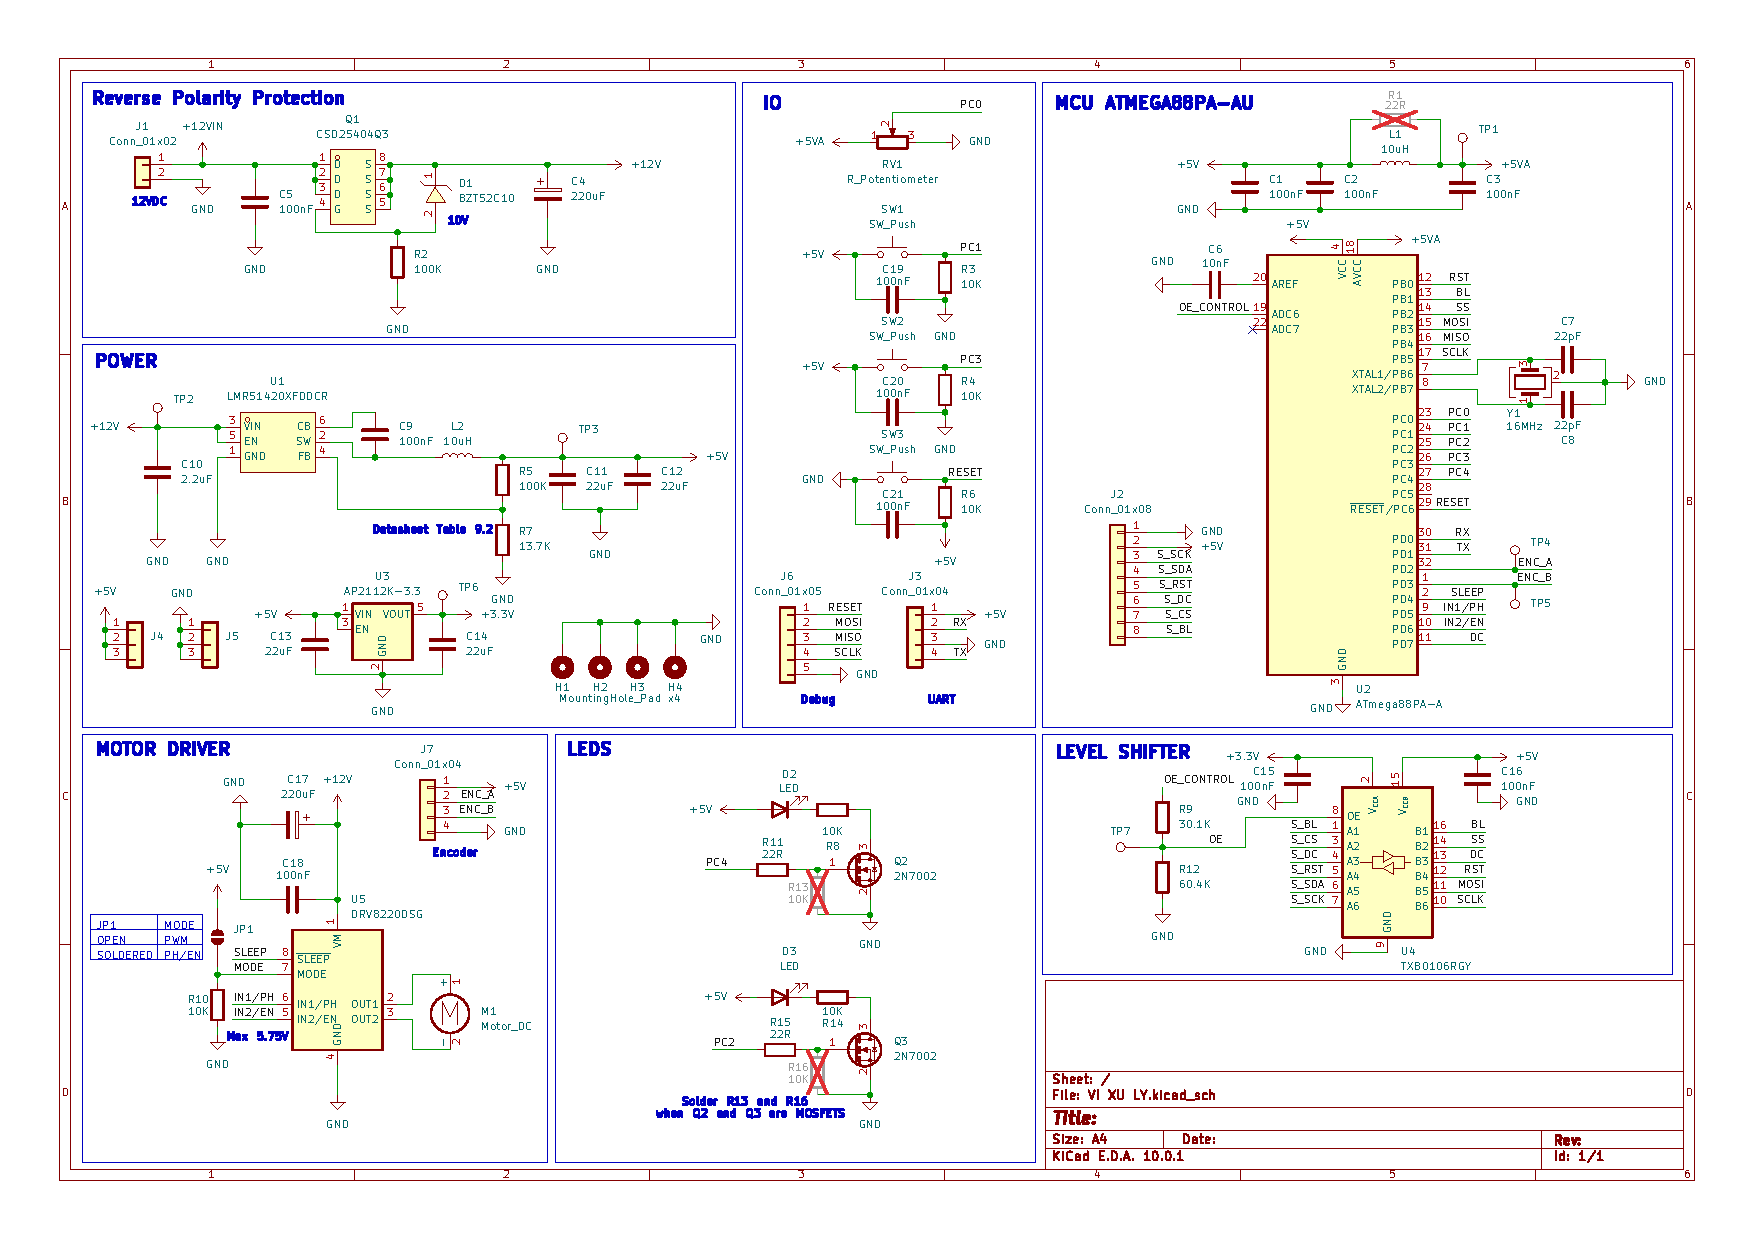
\includegraphics[height=\linewidth,angle=90,page=1]{sch/VIXULY_schematic.pdf}
\end{center}

\chapter{Danh sách linh kiện đầy đủ (BOM)}
\label{app:bom}

Bảng~\ref{tab:bom} là danh sách linh kiện đầy đủ của \proj{}, bao gồm cả linh kiện thụ động, nút nhấn và đầu nối, được trích trực tiếp từ sơ đồ nguyên lý KiCad và nhóm theo khối chức năng.

{\small
\begin{longtable}{@{}>{\raggedright\arraybackslash}p{2.2cm}>{\raggedright\arraybackslash}p{3.5cm}>{\raggedright\arraybackslash}p{2.8cm}c>{\raggedright\arraybackslash}p{5.1cm}@{}}
\caption{Danh sách linh kiện đầy đủ (BOM) của \proj}\label{tab:bom}\\
\toprule
\textbf{Ký hiệu} & \textbf{Giá trị / Mã} & \textbf{Vỏ (footprint)} & \textbf{SL} & \textbf{Chức năng}\\
\midrule\endfirsthead
\toprule
\textbf{Ký hiệu} & \textbf{Giá trị / Mã} & \textbf{Vỏ (footprint)} & \textbf{SL} & \textbf{Chức năng}\\
\midrule\endhead
\bottomrule\endfoot
\multicolumn{5}{@{}l}{\cellcolor{blkfill}\textit{Khối xử lý trung tâm}}\\
U2 & ATmega88PA-A & TQFP-32 & 1 & Vi điều khiển chính\\
Y1 & \SI{16}{\mega\hertz} & SMD 3225 & 1 & Thạch anh dao động\\
C7, C8 & \SI{22}{\pico\farad} & 0603 & 2 & Tụ tải thạch anh\\
L1 / R1 & \SI{10}{\micro\henry} / \SI{22}{\ohm} & 0603 & 2 & Lọc nguồn AVCC (+5VA)\\
C1--C3, C6 & \SI{100}{\nano\farad}, \SI{10}{\nano\farad} & 0603 & 4 & Tụ thoát VCC/AVCC/AREF\\
SW3, R6, C21 & Nút nhấn, \SI{10}{\kilo\ohm}, \SI{100}{\nano\farad} & B3F, 0603 & 3 & Mạch RESET\\
\multicolumn{5}{@{}l}{\cellcolor{pwrfill}\textit{Khối nguồn và bảo vệ}}\\
Q1 & CSD25404Q3 & VSON-8 3,3$\times$3,3 & 1 & P-MOSFET chống ngược cực\\
D1 & BZT52C10 & SOD-123 & 1 & Zener kẹp $V_{GS}$ của Q1\\
R2 & \SI{100}{\kilo\ohm} & 0603 & 1 & Điện trở cực cổng Q1\\
U1 & LMR51420XFDDCR & SOT-23-6 & 1 & Buck đồng bộ \SI{12}{\volt}$\to$\SI{5}{\volt}\\
L2 & \SI{10}{\micro\henry} & IHLP-1616 & 1 & Cuộn cảm buck\\
R5, R7 & \SI{100}{\kilo\ohm}, \SI{13.7}{\kilo\ohm} & 0603 & 2 & Cầu phân áp hồi tiếp (FB)\\
C9, C10, C11, C12 & \SI{100}{\nano\farad}, \SI{2.2}{\micro\farad}, 2$\times$\SI{22}{\micro\farad} & 0603/1206 & 4 & Bootstrap, tụ vào, tụ ra\\
U3 & AP2112K-3.3 & SOT-23-5 & 1 & LDO \SI{3.3}{\volt} / \SI{600}{\milli\ampere}\\
C13, C14 & \SI{22}{\micro\farad} & 1206 & 2 & Tụ vào/ra LDO\\
C4, C17 & \SI{220}{\micro\farad} & Hóa 6,3$\times$7,7 & 2 & Tụ bulk bus \SI{12}{\volt}\\
\multicolumn{5}{@{}l}{\cellcolor{blkfill}\textit{Khối công suất}}\\
U5 & DRV8220DSG & WSON-8 2$\times$2 & 1 & Cầu H \SI{18}{\volt}/\SI{1.76}{\ampere}\\
JP1, R10 & Jumper hàn, \SI{10}{\kilo\ohm} & -- & 2 & Chọn chế độ PWM / PH-EN\\
C18 & \SI{100}{\nano\farad} & 0603 & 1 & Tụ thoát VM\\
M1 & Domino 2 chân & MKDS 5,08 & 1 & Đầu ra động cơ\\
\multicolumn{5}{@{}l}{\cellcolor{iofill}\textit{Khối giao diện}}\\
U4 & TXB0106RGY & VQFN-16 & 1 & Chuyển mức \SI{5}{\volt}$\leftrightarrow$\SI{3.3}{\volt} cho TFT\\
R9, R12 & \SI{30.1}{\kilo\ohm}, \SI{60.4}{\kilo\ohm} & 0603 & 2 & Phân áp chân OE\\
C15, C16 & \SI{100}{\nano\farad} & 0603 & 2 & Tụ thoát VCCA/VCCB\\
RV1 & Chiết áp Alps RK097 & -- & 1 & Đặt tốc độ\\
SW1, SW2 & Nút nhấn Omron B3F & -- & 2 & Nút RUN, STOP\\
R3, R4, C19, C20 & \SI{10}{\kilo\ohm}, \SI{100}{\nano\farad} & 0603 & 4 & Kéo xuống + lọc RC nút nhấn\\
D2, D3 & LED & 1206 & 2 & LED STOP, RUN\\
Q2, Q3 & 2N7002 & SOT-23 & 2 & Khóa LED\\
R8, R11, R13--R16 & \SI{10}{\kilo\ohm}, \SI{22}{\ohm} & 0603 & 6 & Trở hạn dòng LED, trở cổng\\
\multicolumn{5}{@{}l}{\cellcolor{swfill}\textit{Đầu nối và cơ khí}}\\
J1 & Domino 2 chân & MKDS 5,08 & 1 & Đầu vào nguồn \SI{12}{\volt}\\
J2 & Header cái 1$\times$8 & 2,54 mm & 1 & Module TFT WeAct ST7735\\
J3 & JST-XH 4 chân & 2,50 mm & 1 & UART\\
J6 & JST-XH 5 chân & 2,50 mm & 1 & Nạp ISP\\
J7 & JST-XH 4 chân & 2,50 mm & 1 & Encoder\\
J4, J5 & Header 1$\times$3 & 2,54 mm & 2 & Đầu chờ +5V / GND\\
TP1--TP7 & Test point & $\varnothing$\SI{1}{\milli\metre} & 7 & Điểm đo\\
H1--H4 & Lỗ M3 & $\varnothing$\SI{3.2}{\milli\metre} & 4 & Lỗ bắt vít\\
\end{longtable}
}

\chapter{Layout mạch in}
\label{app:layout}

\begin{figure}[H]
\centering
\hinh[0.95\linewidth]{figures/Layout_Front.png}{Layout lớp trên}
\caption{Layout lớp trên (F.Cu) -- kích thước đầy đủ}
\end{figure}

\begin{figure}[H]
\centering
\hinh[0.95\linewidth]{figures/Layout_Back.png}{Layout lớp dưới}
\caption{Layout lớp dưới (B.Cu) -- kích thước đầy đủ}
\end{figure}

\begin{table}[H]
\centering\small
\caption{Danh sách tệp sản xuất (Gerber)}
\begin{tabular}{@{}ll@{}}
\toprule
\textbf{Tệp} & \textbf{Nội dung}\\
\midrule
\texttt{VI XU LY-F\_Cu.gbr} / \texttt{-B\_Cu.gbr} & Lớp đồng trên / dưới\\
\texttt{VI XU LY-F\_Mask.gbr} / \texttt{-B\_Mask.gbr} & Mặt nạ hàn\\
\texttt{VI XU LY-F\_Silkscreen.gbr} / \texttt{-B\_Silkscreen.gbr} & Lớp in lụa\\
\texttt{VI XU LY-F\_Paste.gbr} / \texttt{-B\_Paste.gbr} & Lớp kem hàn (stencil)\\
\texttt{VI XU LY-Edge\_Cuts.gbr} & Đường viền bo mạch\\
\texttt{VI XU LY.drl}, \texttt{VI XU LY-drl\_map.gbr} & Tệp khoan và bản đồ khoan\\
\texttt{VI XU LY-job.gbrjob} & Tệp mô tả công việc (Gerber job)\\
\bottomrule
\end{tabular}
\end{table}

\chapter{Tài liệu tham khảo}
\label{app:docs}

\begingroup
\makeatletter\let\chapter\@gobbletwo\makeatother
\begin{thebibliography}{99}
\bibitem{atmega} Microchip Technology, \emph{ATmega48PA/88PA/168PA/328P -- 8-bit AVR Microcontroller with 4/8/16/32K Bytes In-System Programmable Flash}, Datasheet.
\bibitem{drv8220} Texas Instruments, \emph{DRV8220 18-V H-Bridge Motor Driver with PWM, PH/EN, and Half-Bridge Control Interfaces and Low-Power Sleep Mode}, SLVSFU5B, 2021.
\bibitem{lmr51420} Texas Instruments, \emph{LMR51420 SIMPLE SWITCHER\textsuperscript{\textregistered} 4.5-V to 36-V, 2-A Synchronous Buck Converter in a SOT-23 Package}, SLUSEF6C, 2022.
\bibitem{csd25404} Texas Instruments, \emph{CSD25404Q3 --20 V P-Channel NexFET\texttrademark{} Power MOSFET}, SLPS570, 2015.
\bibitem{txb0106} Texas Instruments, \emph{TXB0106 6-Bit Bidirectional Level-Shifting and Voltage Translator With Auto-Direction Sensing}, SCES709C, 2025.
\bibitem{ap2112} Diodes Incorporated, \emph{AP2112 600mA CMOS LDO Regulator with Enable}, Datasheet.
\bibitem{st7735} Sitronix, \emph{ST7735S 132RGB$\times$162dot 262K Color with Frame Memory Single-Chip TFT Controller/Driver}, Datasheet.
\bibitem{weact} WeAct Studio, \emph{WeAct ST7735 TFT Module}, \url{https://github.com/WeActStudio/WeAct-ST7735}.
\bibitem{pio} PlatformIO, \emph{PlatformIO Documentation -- Atmel AVR platform}, \url{https://docs.platformio.org}.
\bibitem{arduinoisp} Arduino, \emph{Arduino as ISP and Arduino Bootloaders}, \url{https://docs.arduino.cc/built-in-examples/arduino-isp/ArduinoISP}.
\bibitem{kicad} KiCad EDA, \emph{KiCad Documentation}, \url{https://docs.kicad.org}.
\bibitem{ogata} K. Ogata, \emph{Modern Control Engineering}, 5th ed., Prentice Hall, 2010.
\bibitem{astrom} K. J. Åström, T. Hägglund, \emph{Advanced PID Control}, ISA, 2006.
\bibitem{repo} Nhóm thực hiện, \emph{ME4169 Microprocessor Final term project -- mã nguồn và thiết kế}, \url{https://github.com/1m4n00b6292/ME4169-Microprocessor-Final-term-Project}.
\end{thebibliography}
\endgroup


\end{document}
